\documentclass[12pt,twoside,openright]{report}

\usepackage[a4paper]{geometry}
\usepackage[utf8]{inputenc}
\usepackage[T1]{fontenc}
\usepackage[style=authoryear, citestyle=authoryear, doi=false, url=false, isbn=false]{biblatex}
\usepackage{minitoc}
\usepackage[table]{xcolor}
\usepackage{amssymb,amsmath}
\usepackage{graphicx}
\usepackage{dsfont}
\usepackage{subcaption}
\usepackage{bm}
\usepackage{rotating}
\usepackage{adjustbox}
\usepackage{array}
\usepackage{setspace}
\usepackage{bibentry}
\usepackage{pdfpages}
\usepackage{fancyhdr}
\usepackage{appendix}
\usepackage[Bjornstrup]{fncychap}

\usepackage{hyperref}

%%%%%%%%%%%%%%%%%%%%%%%%%%%%%%%%%%%%%%%%%%%%%%%%%%%%%%%%%%%%%%%%%%%%%%%%%%%%%%%%%%%%%%%%%%%%%%%
%                                SETUP AND MACRO DECLARATIONS                                 %
%%%%%%%%%%%%%%%%%%%%%%%%%%%%%%%%%%%%%%%%%%%%%%%%%%%%%%%%%%%%%%%%%%%%%%%%%%%%%%%%%%%%%%%%%%%%%%%

% Color definitions from: http://latexcolor.com/
\definecolor{alizarin}{rgb}{0.82, 0.1, 0.26}
\definecolor{azure}{rgb}{0.0, 0.5, 1.0}
\definecolor{deeplilac}{rgb}{0.6, 0.33, 0.73}

% Hyperref setup
\hypersetup{
    linktoc=all,
    linktocpage=true,
    colorlinks=true,
    linkcolor=azure,
    urlcolor=alizarin
}

% Redefine cite and textcite so author + year clickable in the color I want
\newcommand\mkbibcolor[2]{\textcolor{#1}{\hypersetup{citecolor=}#2}}  
\DeclareCiteCommand{\cite}[\mkbibcolor{deeplilac}]
  {\usebibmacro{prenote}}
  {\usebibmacro{citeindex}%
   \printtext[bibhyperref]{\usebibmacro{cite}}}
  {\multicitedelim}
  {\usebibmacro{postnote}}
  
\DeclareCiteCommand{\textcite}[\mkbibcolor{deeplilac}]
  {\boolfalse{cbx:parens}}
  {\usebibmacro{citeindex}%
   \printtext[bibhyperref]{\usebibmacro{textcite}}}
  {\ifbool{cbx:parens}
     {\bibcloseparen\global\boolfalse{cbx:parens}}
     {}%
   \multicitedelim}
  {\usebibmacro{textcite:postnote}}
  
% Bibmacro manipulation to have author name as link to paper
\newcommand{\letbibmacro}[2]{%
  \csletcs{abx@macro@#1}{abx@macro@#2}%
}
\letbibmacro{orig-author}{author}
\renewbibmacro*{author}[1]{%
  \iffieldundef{doi}{%
    \iffieldundef{url}{%
      \iffieldundef{isbn}{%
        \iffieldundef{issn}{\mkbibbold\bgroup\usebibmacro{orig-author}\egroup
        }{%
          \href{http://books.google.com/books?vid=ISSN\thefield{issn}}{\mkbibbold\bgroup\usebibmacro{orig-author}\egroup}%
        }%
      }{%
        \href{http://books.google.com/books?vid=ISBN\thefield{isbn}}{\mkbibbold\bgroup\usebibmacro{orig-author}\egroup}%
      }%
    }{%
      \href{\thefield{url}}{\mkbibbold\bgroup\usebibmacro{orig-author}\egroup}%
    }%
  }{%
    \href{http://dx.doi.org/\thefield{doi}}{\mkbibbold\bgroup\usebibmacro{orig-author}\egroup}%
  }%
}

% Remove In: in bibliography
\renewbibmacro{in:}{}

% Augment space between entries in the bibliography
\setlength\bibitemsep{1.2\itemsep}

% Define chapter abstract
\newenvironment{chapabstract}{%
    \begin{large}%
      \bfseries Abstract \\
    \end{large}
% 	\textbf{Abstract}
    }%
   {\par}
  
% Math
\DeclareMathOperator*{\argmin}{argmin}

% Text spacing
\renewcommand{\baselinestretch}{1.1}

% Confusion matrix
% https://tex.stackexchange.com/questions/20267/how-to-construct-a-confusion-matrix-in-latex
\usepackage{collcell}
\usepackage{hhline}
\usepackage{pgf}
\usepackage{multirow}

\def\colorModel{hsb} %You can use rgb or hsb

\newcommand\ColCell[1]{
  \pgfmathparse{#1<50?1:0}  %Threshold for changing the font color into the cells
    \ifnum\pgfmathresult=0\relax\color{white}\fi
  \pgfmathsetmacro\compA{0}      %Component R or H
  \pgfmathsetmacro\compB{#1/100} %Component G or S
  \pgfmathsetmacro\compC{1}      %Component B or B
  \edef\x{\noexpand\centering\noexpand\cellcolor[\colorModel]{\compA,\compB,\compC}}\x #1
  } 
\newcolumntype{E}{>{\collectcell\ColCell}m{0.4cm}<{\endcollectcell}}  %Cell width
\newcommand*\rot{\rotatebox{90}}

% subsubsection numbering
\setcounter{secnumdepth}{3}

% Rotation in array
\newcolumntype{R}[2]{%
    >{\adjustbox{angle=#1,lap=\width-(#2)}\bgroup}%
    l%
    <{\egroup}%
}
\newcommand*\rota{\multicolumn{1}{R{45}{1em}}}

%%%%%%%%%%%%%%%%%%%%%%%%%%%%%%%%%%%%%%%%%%%%%%%%%%%%%%%%%%%%%%%%%%%%%%%%%%%%%%%%%%%%%%%%%%%%%%%

\title{Thesis}
\author{Hadrien Bertrand}

\addbibresource{publi.bib}
\addbibresource{references.bib}

\includeonly{chap_introduction, chap_segmentation, chap_transfer_learning, chap_hyperopt, chap_conclusion, appendix_cholesky}
% \includeonly{chap_hyperopt}

\pagenumbering{roman}

\begin{document}
\begin{titlepage}
    
\includepdf{cover/1ere}
\end{titlepage}

\cleardoublepage

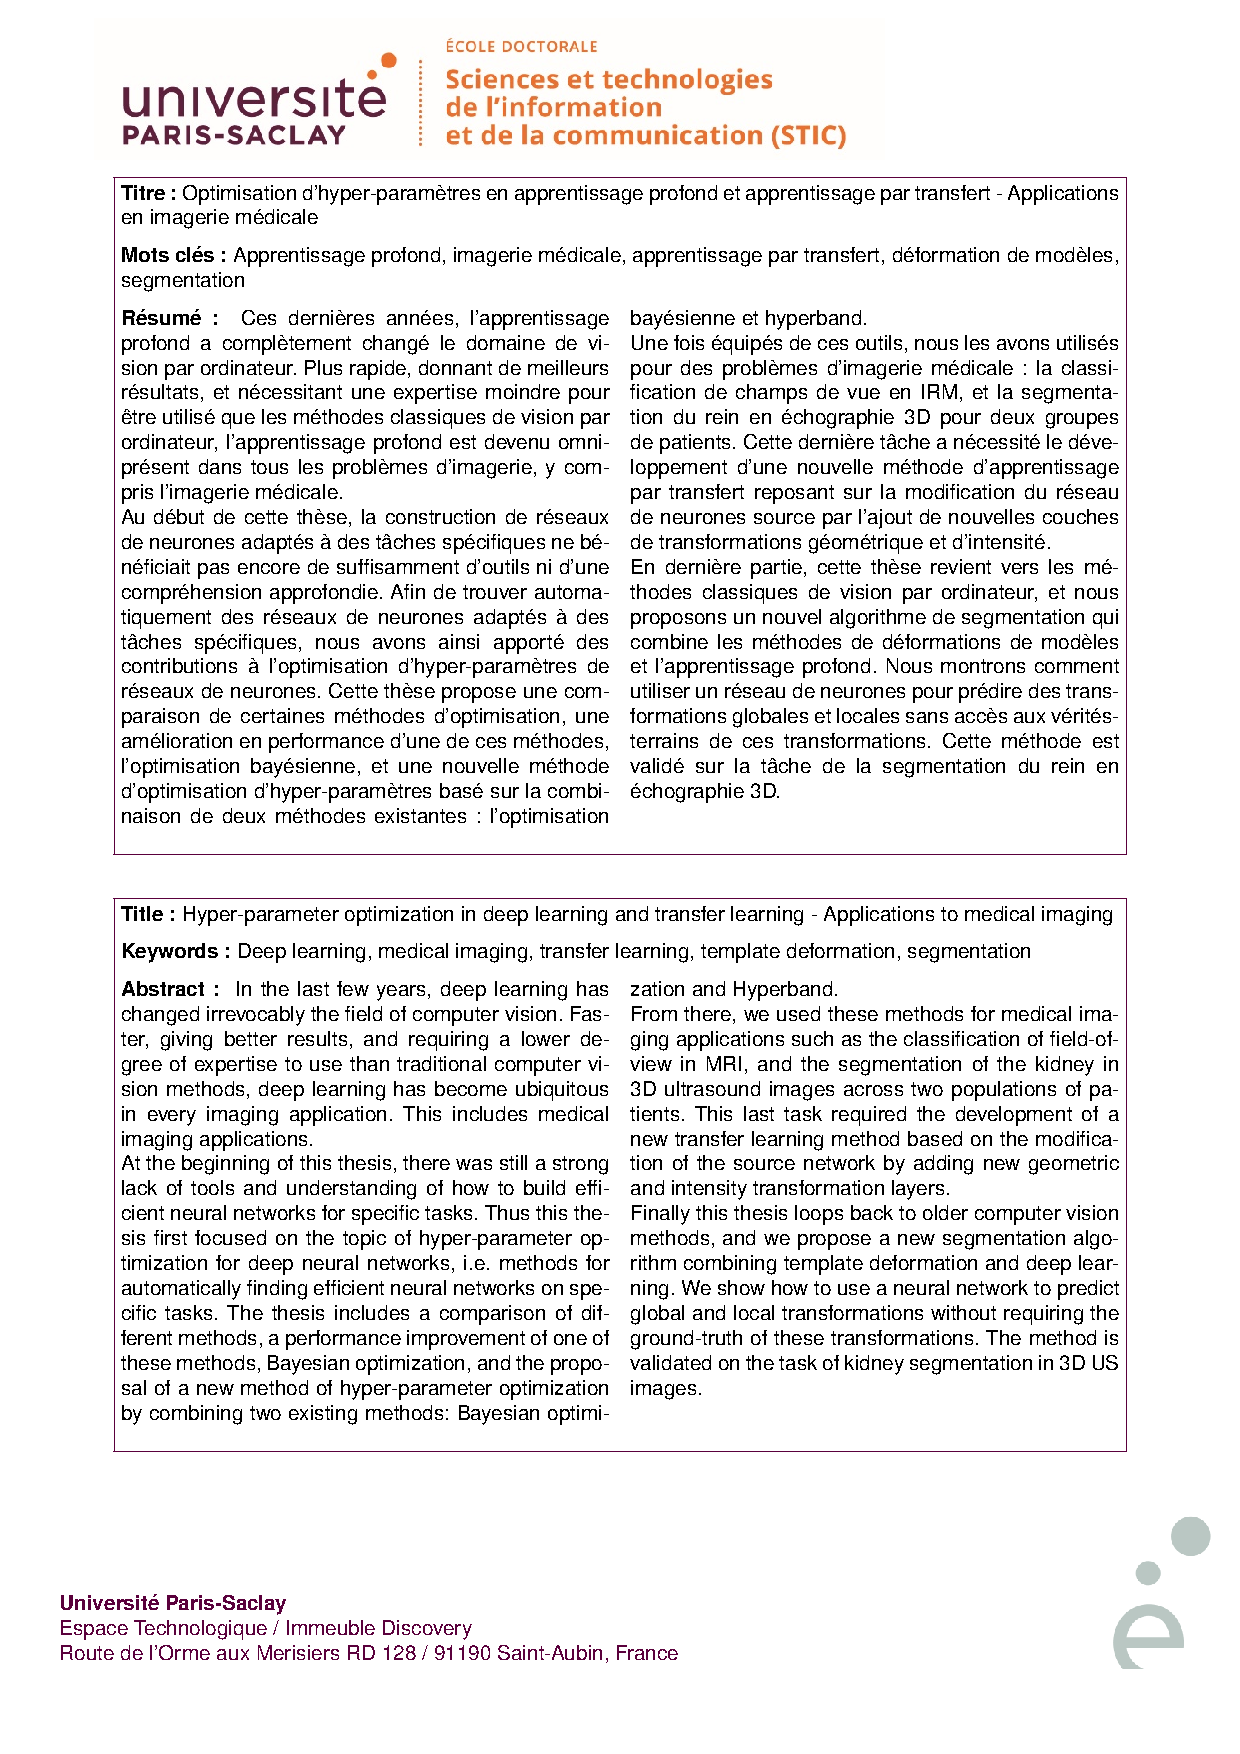
\includepdf{cover/4eme}

\cleardoublepage

\dominitoc
{   
    \setstretch{1.1}
    \tableofcontents
}

\cleardoublepage

\listoffigures

\clearpage
 
\listoftables

\cleardoublepage

\pagenumbering{arabic}

% fancy style
\pagestyle{fancy}
\fancyhf{}
%\fancyhead[R]{\thepage}
\fancyhead[LE]{\fontsize{10}{12} \selectfont \slshape \rightmark}
\fancyhead[RO]{\fontsize{10}{12} \selectfont \slshape \leftmark}
\fancyhead[LO,RE]{\thepage}
\setlength{\headheight}{30pt}

%%%%%%%%%%%%%%%%%%%%%%%%%%%%%%%%%%%%%%%%%%%%%%%%%%%%%%%%%%%%%%%%%%%%%%%%%%%%%%%%%%%%%%%%%%%%%%%
%                                        INTRODUCTION                                         %
%%%%%%%%%%%%%%%%%%%%%%%%%%%%%%%%%%%%%%%%%%%%%%%%%%%%%%%%%%%%%%%%%%%%%%%%%%%%%%%%%%%%%%%%%%%%%%%
\chapter{Introduction}
\label{chap:intro}

\minitoc

\newpage

%%%%%%%%%%%%%%%%%%%%%%%%%%%%%%%%%%%%%%%%%%%%%%%%%%%%%%%%%%%%%%%%%%%%%%%%%%%%%%%%%%%%%%%%%%%%%%%
\section{Context}

%%%%%%%%%%%%%%%%%%%%%%%%%%%%%%%%%%%%%%%%%%%%%%%%%%%%%%%%%%%%%%%%%%%%%%%%%%%%%%%%%%%%%%%%%%%%%%%
\section{Medical Imaging}

\subsection{Common tasks}

Classification, segmentation, localization

How it's useful to physician.

\subsection{Specificity of Medical Images}

CT, MR, US
vs
natural images

\subsection{Challenges}

Lack of data

Sensitivity of the data

Effects of different protocols, machines, physicians on the images...

Interpretability of the results

%%%%%%%%%%%%%%%%%%%%%%%%%%%%%%%%%%%%%%%%%%%%%%%%%%%%%%%%%%%%%%%%%%%%%%%%%%%%%%%%%%%%%%%%%%%%%%%
\section{Deep Learning}

Fast moving field, results are obsolete fast.

%%%%%%%%%%%%%%%%%%%%%%%%%%%%%%%%%%%%%%%%%%%%%%%%%%%%%%%%%%%%%%%%%%%%%%%%%%%%%%%%%%%%%%%%%%%%%%%
\section{Transfer Learning}

%%%%%%%%%%%%%%%%%%%%%%%%%%%%%%%%%%%%%%%%%%%%%%%%%%%%%%%%%%%%%%%%%%%%%%%%%%%%%%%%%%%%%%%%%%%%%%%
\section{Contributions}

%%%%%%%%%%%%%%%%%%%%%%%%%%%%%%%%%%%%%%%%%%%%%%%%%%%%%%%%%%%%%%%%%%%%%%%%%%%%%%%%%%%%%%%%%%%%%%%
\section{Outline}

Structure of the thesis


%%%%%%%%%%%%%%%%%%%%%%%%%%%%%%%%%%%%%%%%%%%%%%%%%%%%%%%%%%%%%%%%%%%%%%%%%%%%%%%%%%%%%%%%%%%%%%%
%                                          HYPEROPT                                           %
%%%%%%%%%%%%%%%%%%%%%%%%%%%%%%%%%%%%%%%%%%%%%%%%%%%%%%%%%%%%%%%%%%%%%%%%%%%%%%%%%%%%%%%%%%%%%%%
\chapter{Hyper-parameter Optimization of Neural Networks}
\label{chap:hyperopt}

\begin{chapabstract}
This chapter introduces the problem of hyper-parameter optimization for neural networks, which is the problem of automatically finding the optimal architecture and training setting for a particular task. Section~\ref{sec:ho_lit} presents the problem and the existing approaches while Section~\ref{sec:bo} explains in depth the method of Bayesian optimization which is used for the rest of the chapter. A performance improvement of this method is given in Section~\ref{sec:cholesky}. In Section~\ref{sec:compare}, we compare the performance of random search and Bayesian optimization on a toy problem and give theoretical bounds on the performance of random search. We propose a new method in Section~\ref{sec:cap}, which combines Bayesian optimization with another method, Hyperband. Finally, we apply Bayesian optimization to the practical problem of MRI field-of-view classification in Section~\ref{sec:isbi}.
\end{chapabstract}

\vspace{1cm}

{   
    \setstretch{1.0}
    \minitoc
}

\newpage

%%%%%%%%%%%%%%%%%%%%%%%%%%%%%%%%%%%%%%%%%%%%%%%%%%%%%%%%%%%%%%%%%%%%%%%%%%%%%%%%%%%%%%%%%%%%%%%
\section{Defining the Problem}
\label{sec:ho_lit}

The problem of hyper-parameter optimization appears when a model is governed by numerous hyper-parameters that are difficult to manually tune due to a lack of understanding of their effects. The problem gets worse when the hyper-parameters are not independent and it becomes necessary to tune them at the same time. The most intuitive solution is to test all possible combinations, but its number grows exponentially with the number of hyper-parameters, making this approach usually unusable for neural networks.

In practice, as it is usually impossible to prove the optimality of a solution without testing all solutions, the accepted solution is the best found in the budget allocated by the user to the search.

Even though this problem appears in all kinds of situations, we are interested here in the optimization of deep learning models, as they have many hyper-parameters and we lack the understanding and the theoretical tools to tune them.

%%%%%%%%%%%%%%%%%%%%%%%%%%%%%%%%%%
\subsection{Notations}
\label{ssec:notation}

In this chapter we refer to a \textit{model} as a neural network, even though the black-box methods presented in Section~\ref{ssec:black_box} work for other machine learning models. The \textit{parameters} of a model are the weights of the network which are learned during training. The \textit{hyper-parameters} are the parameters governing the architecture of the networks (such as the number of layers or the type of layers) and the ones governing the training phase (such as the learning rate or the batch size). 

A \textit{hyper-parameter space} $\mathrm{X}$ is a hypercube where each dimension is a hyper-parameter and the boundaries of the hypercube are the boundaries of each hyper-parameter. Each point in the hyper-parameter space is referred to as a \textit{combination} $\mathrm{x} \in \mathrm{X}$. To each combination is associated a value $\mathrm{y}$ corresponding to the performance metric of the underlying neural network on the task it is trained to solve. We name $f$ a function taking as input a combination $\mathrm{x}$, build and train the underlying model and output its performance $f\left( \mathrm{x} \right)$.

%%%%%%%%%%%%%%%%%%%%%%%%%%%%%%%%%%
\subsection{Black-box optimization}
\label{ssec:black_box}

From the notation of Section~\ref{ssec:notation}, the goal of hyper-parameter optimization is to find the combination $\mathrm{x_*}$ minimizing the performance $\mathrm{y}$ (typically the performance is a loss function, which we want to minimize):
\begin{equation}
	\mathrm{x_*} = \argmin_{\mathrm{x} \in \mathrm{X}} f(\mathrm{x})
\end{equation}

This is the problem of hyper-parameter optimization viewed as black-box optimization. Methods in this category are independent from the model and could be used for any kind of mathematical function. However the hyper-parameters we are interested in are of a varied nature (continuous, discrete, categorical), limiting us to derivative-free optimization methods. This section is not a complete review of derivative-free algorithms, but an overview of the popular algorithms used specifically for hyper-parameter optimization.

Additionally, since the function $f$ is a process training a neural network, evaluating a combination is costly in time and computing resources. Moreover we have little understanding of the influence of each hyper-parameter on the performance of the model, resulting in very large boundaries and a much bigger space than needed. The situation is even worse since combinations near the boundaries of the hyper-parameter space can build a network too big to fit in the available memory, requiring to have a way to handle evaluation failures. 

While it is tempting to simply return an extremely bad performance, this causes problems to methods assuming some structure in the hyper-parameter space. For example, a continuous hyper-parameter that gives a smooth output will suddenly have a discontinuity, and a method assuming smoothness might not work anymore. In practice, there are method-dependent solutions to this problem.

\subsubsection{Grid search}

The most basic method is usually called \textit{grid search}. Very easy to implement, it simply tests every possible combination (typically with uniform sampling for the continuous hyper-parameters). With only a handful of hyper-parameters to optimize and with a function $f$ fast to evaluate, it can be advisable to use as a first step to get sensible boundaries on each hyper-parameter, i.e. by testing a handful of values over a very wide range to find a smaller but relevant range.

But in the context of deep learning, hyper-parameters are too numerous, meaning there are too many combinations to evaluate, and each evaluation is costly. Also, a typical implementation in nested for-loops goes from one corner of the hyper-parameter space to the opposite corner in order. It is unlikely that the corner the search starts from happens to be an area filled with good models, since combinations in corners are extreme values of hyper-parameters and build atypical neural networks. 

Grid search can still be used with a wide enough sampling of the hyper-parameters to get an idea on where the interesting models are located and refine the boundaries, but even for that other methods are preferable.

\subsubsection{Random search}

One step above grid search is \textit{random search}. A big limitation of grid search is that the order it goes through the hyper-parameter space is very dependent on the implementation and it always selects the same limited set of values for each hyper-parameter. Random search instead draws the value of each hyper-parameter from a uniform distribution, allowing for a much wider range of explored values.

\begin{figure}[htb]
	\begin{minipage}[b]{.49\linewidth}
		\centering
		\centerline{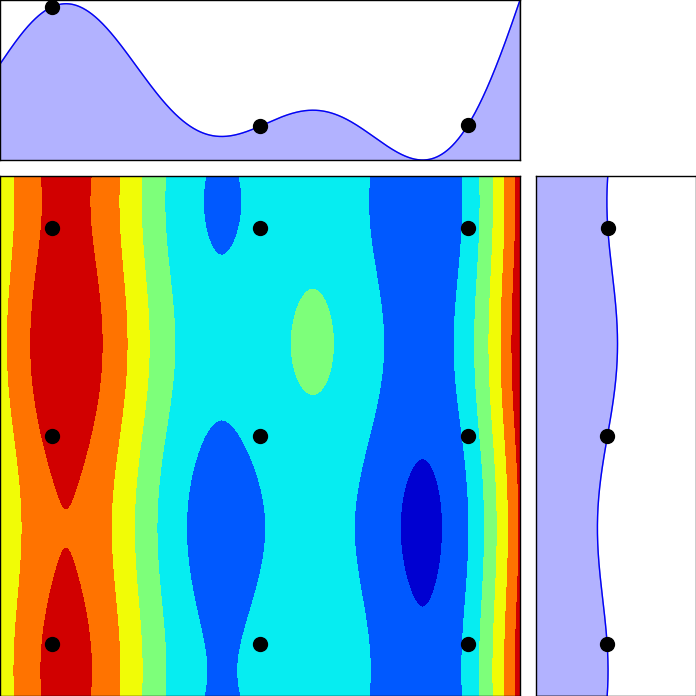
\includegraphics[width=7.2cm]{img_hyperopt/rs_grid}}
	\end{minipage}
	\begin{minipage}[b]{.49\linewidth}
		\centering
		\centerline{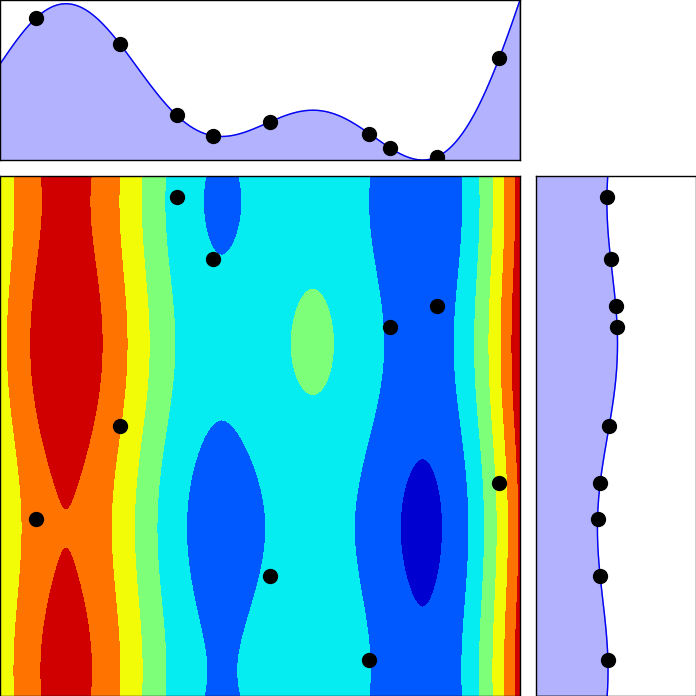
\includegraphics[width=7.2cm]{img_hyperopt/rs_random}}
	\end{minipage}
	\caption{Loss function for a two dimensional space. (Left) Grid search. (Right) Random search. 9 combinations were tested for each method, but grid search tested only 3 values for each hyper-parameters while random search tested 9, resulting in a better solution.}
	\label{fig:rs}
\end{figure}

Figure~\ref{fig:rs} illustrates this. Given a hyper-parameter space of two continuous hyper-parameters, and at equal number of evaluated combinations, random search finds a better solution. It works because hyper-parameters are not equally relevant. In practice, only a few have a high impact on the performance (\textcite{bergstra2012JMLR}). In the figure, grid search only tested three values of each hyper-parameters while random search tested nine for the same cost!

In terms of implementation cost, random search requires only the ability to draw uniformly from an interval or a list, making it barely more costly than grid search, largely compensated by the gain in performance.

\subsubsection{Bayesian optimization}

Going further requires some assumption about the structure of the hyper-parameter space. Namely, similar values for an hyper-parameter results in similar performance, i.e. some weak notion of continuity. If there is some structure, we can exploit it.

Bayesian optimization (\textcite{bergstra2011NIPS}), which we present in details in Section~\ref{sec:bo}, applies this idea by modeling $f$ with as few evaluations as possible while searching for the best combination. It comes with a non-trivial implementation cost, though packages are available. In Section~\ref{sec:compare} we compare the performance of random search and Bayesian optimization on a practical task.

%%%%%%%%%%%%%%%%%%%%%%%%%%%%%%%%%%
\subsection{Evolutionary algorithms}

The first application of evolutionary algorithms to neural networks was to evolve the weights of a fixed architecture (\textcite{miller1989}). A few years later,~\textcite{braun1993} and~\textcite{angeline1994} realized it was more efficient to evolve simultaneously the weights and the topology of the network. Further refinements of these approaches led to the \textit{NeuroEvolution of Augmenting Topologies} (NEAT) algorithm (\textcite{stanley2002EC}). 

NEAT uses three kinds of mutations (modifying a weight, adding a connection between two nodes and adding a node in the middle of a connection) and one kind of recombination based on fitness sharing. Many variants of this algorithm have been proposed, notably HyperNEAT (\textcite{stanley2009}) which only evolves the topology and learns the weights by back-propagation. 

The main drawback of NEAT and its variants is their inability to scale and evolve the large networks typical of modern deep learning.~\textcite{real2017ICML} and~\textcite{miikkulainen2017} developed approaches able to explore extremely diverse and atypical network structures and find architectures with state-of-the-art performance on computer vision tasks such as CIFAR-10. The drawback of those methods however is their excessive computational cost, making them out of our reach.

%%%%%%%%%%%%%%%%%%%%%%%%%%%%%%%%%%
\subsection{Reinforcement learning}

Recent advances in reinforcement learning have made possible its use to design efficient neural networks. The idea is to train an agent called the controller which builds neural networks for a specific task.~\textcite{baker2017ICLR} developed a controller that chooses each layer of the network sequentially and is trained using Q-learning.~\textcite{zoph2017ICLR} created a string representation of neural networks and their controller is a RNN outputting valid strings. In both cases the created networks must be fully trained to be evaluated and the controller takes thousands of iterations to converge, making those approaches extremely costly.

To address this problem,~\textcite{zoph2017} proposed testing on a smaller dataset as an approximation of the performance on the true dataset. Another suggestion is to train only partially each network (\textcite{li2017ICLR},~\textcite{zela2018}), allowing longer training time as the search is refined.

%%%%%%%%%%%%%%%%%%%%%%%%%%%%%%%%%%
\subsection{Other approaches}

We finish our tour with a few methods taking radically different approaches. Hyperband (\textcite{li2017ICLR}) considers the question as a multi-armed bandit problem, where each arm is a combination and we have a finite amount of training budget to allocate to each arm. The idea is to train many models partially, and take the decision to continue training every few epochs based on the current performance. We present it in more details in Section~\ref{ssec:hyperband}.

\textcite{hazan2018ICLR} proposed an approach applying compressed sensing to hyper-parameters optimization called Harmonica. Like Bayesian optimization, they aim to learn the structure of the hyper-parameter space, but using a sparse polynomial as the model.

Finally,~\textcite{domhan2015} suggested predicting the learning curve of a model to decide whether to continue the training. The prediction is done using a portfolio of parametric models.

%%%%%%%%%%%%%%%%%%%%%%%%%%%%%%%%%%
\subsection{Synthesis}
\label{ssec:synthesis}

\begin{sidewaystable}[htbp]
	\centering
	\begin{tabular}{ | l | c | c | c | c | c | c | c | c | c | }
		 \rota{} & \rota{Grid Search} & \rota{Random Search} & \rota{Bayesian Optimization - GP} & \rota{Bayesian Optimization - Tree} & \rota{Evolutionary Algorithms} & \rota{Reinforcement Learning} & \rota{Extrapolation of Learning Curves} & \rota{Hyperband} & \rota{Harmonica} \\ 
		\hline
		Black-box? & \checkmark & \checkmark & \checkmark & \checkmark & & & & & \checkmark \\
		Does not require structure in $\mathrm{X}$? & \checkmark & \checkmark & & & & & & \checkmark & \\
		Conditional hyper-parameters? & & & & \checkmark & \checkmark & \checkmark & & & \\
		Training method hyper-parameters? & \checkmark & \checkmark & \checkmark & \checkmark & & & $\checkmark^1$ & $\checkmark^1$ & \checkmark \\
		Easy to parallelize? & & \checkmark & & & \checkmark & \checkmark & & \checkmark & \\
		Method complexity? & Low & Low & Mid & Mid & High & High & Mid & Mid & High \\
		Budget required? & Mid & Mid & Low & Low & High\textsuperscript{2} & High\textsuperscript{2} & Low & Mid & Low \\
		\hline
	\end{tabular}
	\caption{Comparison of different hyper-parameter optimization methods according to various criteria explained in Section~\ref{ssec:synthesis}. (1) Except for the number of epochs or training time which is controlled by the method. (2) This is quickly being reduced.}
	\label{table:hyperopt_compare}
\end{sidewaystable}

We have presented a variety of methods that have been used to optimize the hyper-parameters of neural networks. We summarize their advantages and differences in Table~\ref{table:hyperopt_compare} according to several important criteria.

By black-box we ask whether the method makes any assumption about the model being optimized. Those are the methods that can be reused without modifications to optimize other machine learning models. The second criterion is if the method requires some structure in the hyper-parameter space to work. Would the method still work if we randomize the mapping from combination to performance? 

The next two criteria are about the kind of hyper-parameters the method can work with. By conditional hyper-parameter we mean hyper-parameters whose relevance depends on the value of another hyper-parameter, for example the number of filters of a convolutional layer is only relevant if the layer exists. The second class of hyper-parameters are the one altering the training of the model instead of its topology, such as the learning rate or the batch size. 

The last three criteria are subjective but relevant when choosing a method to use. If the method allows training multiple models at the same time (therefore allowing using many GPUs) without major changes, we consider it easily parallelizable. The difficulty of understanding and implementing the method is evaluated on a coarse low to high scale. We use the same scale for the budget required to find some of the best models of a hyper-parameter space.

%%%%%%%%%%%%%%%%%%%%%%%%%%%%%%%%%%
\subsection{Conclusion}

The first methods used for the optimization of hyper-parameters in neural networks were, without surprise, existing hyper-parameters optimization methods treating the model as black-box and which were developed for other models. While still competitive, they are limited in the architectures of networks they can explore, often working at a layer-level. 

Modern approaches based on evolutionary algorithms or reinforcement learning focus on much more fine-grained architecture choices, at the unit-level. This shift from optimizing hyper-parameters to building architecture is marked notably by the problem increasingly being called Neural Architecture Search. While those methods are too resource intensive to be used in most cases, this is changing very rapidly. 

But in the context of this thesis we worked with what was the most relevant at the time, namely Bayesian optimization, and to some extent, Hyperband.

%%%%%%%%%%%%%%%%%%%%%%%%%%%%%%%%%%%%%%%%%%%%%%%%%%%%%%%%%%%%%%%%%%%%%%%%%%%%%%%%%%%%%%%%%%%%%%%
\section{Bayesian Optimization}
\label{sec:bo}

Bayesian Optimization is a method for optimizing the parameters of a black-box that is costly to evaluate. In deep learning the black-box is a neural network and the parameters are the hyper-parameters of the network. Evaluating the network corresponds to training it and computing its performance on the validation set. A recent and general review of the topic can be found in~\textcite{shahriari2016IEEE} where it is treated as an optimization method, while~\textcite{snoek2012NIPS} review the topic in the context of optimizing the hyper-parameters of machine learning models.

There are two components in Bayesian optimization methods. The first component is a probabilistic model of the loss function, i.e. a function that takes the values of the hyper-parameters as input and estimate the value of the loss the corresponding neural network would have. Gaussian processes are the typical choice and are presented in Section~\ref{ssec:gp}. 
%While other models are available, such as tree-structured Parzen estimators (\textcite{bergstra2011NIPS}), they offer a different set of advantages and weaknesses which we discuss in Section~\ref{ssec:practical}. 
The second component, called the acquisition function, samples the model of the loss function to select the next set of hyper-parameters to evaluate. Common acquisition functions are presented in Section~\ref{ssec:acqfunc}.

%%%%%%%%%%%%%%%%%%%%%%%%%%%%%%%%%%
\subsection{Gaussian processes}
\label{ssec:gp}

A Gaussian process is a supervised learning model mainly used for regression problems. It is a distribution over functions, i.e. from a set of data points, the Gaussian process gives possible functions that fit those points, weighted by their likelihood. The shape and properties of possible functions are defined by a covariance function. When predicting the value of an unseen point, the Gaussian process returns a Normal distribution, with the variance being an estimation of the uncertainty of the model at this point. Predicting multiple points will result in a joint Gaussian distribution. A comprehensive review of the topic can be found in~\textcite{rasmussen2005}

\subsubsection{Definitions}

Following the notation of Section~\ref{ssec:notation}, we write the Gaussian process as:
\begin{equation}
    \mathrm{y}(\mathrm{x}) \sim \mathcal{GP} \left( m(\mathrm{x}), k(\mathrm{x}, \mathrm{x}) \right)
\end{equation}
$m(\mathrm{x})$ is the \textit{mean function} and $k(\mathrm{x}, \mathrm{x'})$ is the \textit{covariance function} which specifies the covariance between pair of data points. The mean function is set to $0$ for simplicity. In practice this is ensured by removing the mean of the predicted values from the dataset. The covariance function is used to build the covariance matrix of a set $\mathrm{X}$ of $N$ data points as:
\begin{equation}
    K(\mathrm{X}, \mathrm{X}) = 
    \begin{pmatrix}
    k(\mathrm{x_1}, \mathrm{x_1}) & k(\mathrm{x_1}, \mathrm{x_2}) & \cdots & k(\mathrm{x_1}, \mathrm{x_N}) \\
    k(\mathrm{x_2}, \mathrm{x_1}) & k(\mathrm{x_2}, \mathrm{x_2}) & \cdots & k(\mathrm{x_2}, \mathrm{x_N}) \\
    \vdots & \vdots & \ddots & \vdots \\
    k(\mathrm{x_N}, \mathrm{x_1}) & k(\mathrm{x_N}, \mathrm{x_2}) & \cdots & k(\mathrm{x_N}, \mathrm{x_N})
    \end{pmatrix}
\end{equation}
This matrix is all that is needed to draw samples from the distribution. We pick a set $\mathrm{X_*}$ of points, build the covariance matrix $K(\mathrm{X_*}, \mathrm{X_*})$, then generate samples from this Gaussian distribution:
\begin{equation}
    \mathrm{y_*} \sim \mathcal{N} \left( 0, K(\mathrm{X_*}, \mathrm{X_*})\right)
\end{equation}
Some such samples are shown in Figure~\ref{fig:gp_prior}. Since no data points were used, this corresponds to an unfitted Gaussian process. 

%The covariance matrix is a Gram matrix, meaning it is positive semi-definite, i.e. it admits a unique Cholesky decomposition

\begin{figure}[htb]
	\centering
	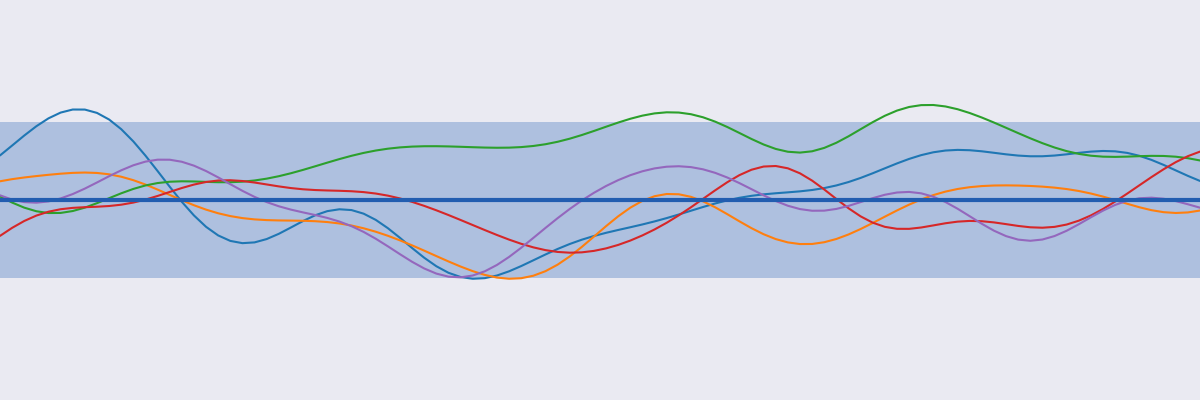
\includegraphics[width=\linewidth]{img_hyperopt/gp_prior.png}
	\caption{Gaussian process prior using a squared exponential kernel. The thin colored lines are samples drawn from the Gaussian process. The thick blue line represents the mean of the distribution and the blue area around this line is the $95 \%$ prediction interval, i.e. all drawn samples will be in this interval with a probability of $95 \%$ (for a Normal distribution this is equal to $1.96 \sigma$)}
	\label{fig:gp_prior}
\end{figure}

In probabilistic terms, the unfitted Gaussian process corresponds to the \textit{prior} probability $p \left( \mathrm{y} \right)$. Given a set of observed points $(\mathrm{X}, \mathrm{y})$ and a set of points we want to predict $(\mathrm{X_*}, \mathrm{y_*})$, the prior corresponds to $p\left( \mathrm{y_*} | \mathrm{X_*}, \theta \right)$, where $\theta$ denote the set of hyper-parameters of the covariance function. We are interested in the \textit{posterior} probability $p\left( \mathrm{y_*} | \mathrm{X_*}, \mathrm{X}, \mathrm{y}, \theta \right)$ i.e. the distribution of the new points conditioned on the points we have already observed. From probability theory we know that the posterior is:
\begin{equation}
    p\left( \mathrm{y_*} | \mathrm{X_*}, \mathrm{X}, \mathrm{y}, \theta \right)
    =
    \frac{p\left( \mathrm{y}, \mathrm{y_*} | \mathrm{X}, \mathrm{X_*}, \theta \right)}{p\left( \mathrm{y} | \mathrm{X}, \theta \right)}
    \label{eq:posterior}
\end{equation}
The numerator is called the \textit{joint distribution} and the denominator is the \textit{marginal likelihood}. 

\subsubsection{Inference}

Training a Gaussian process simply means pre-computing $K(\mathrm{X}, \mathrm{X})$, i.e. the covariance between the data points. At inference, we compute the covariance $K(\mathrm{X_*}, \mathrm{X_*})$ between the points we want to predict, and the covariance between the data points and the points we want to predict $K(\mathrm{X}, \mathrm{X_*})$. Since the covariance matrix is by definition symmetrical, $K(\mathrm{X_*}, \mathrm{X}) = K(\mathrm{X}, \mathrm{X_*})^T$. For notational simplicity we denote them $K$, $K_*$ or $K_*^T$ and $K_{**}$.

This results in the joint distribution of Equation~\ref{eq:posterior}:
\begin{equation}
    \begin{bmatrix}
    \mathrm{y} \\
    \mathrm{y_*}
    \end{bmatrix}
    \sim
    \mathcal{N} \left( 0, 
    \begin{bmatrix}
    K(\mathrm{X}, \mathrm{X}) & K(\mathrm{X}, \mathrm{X_*}) \\
    K(\mathrm{X_*}, \mathrm{X}) & K(\mathrm{X_*}, \mathrm{X_*})
    \end{bmatrix}
    \right)
    =
    \mathcal{N} \left( 0, 
    \begin{bmatrix}
    K & K_*^T \\
    K_* & K_{**}
    \end{bmatrix}
    \right)
\end{equation}
However the joint distribution generate functions that do not match the observed data. The posterior is obtained by conditioning the joint distribution to the observations, which are expressed by the marginal likelihood. Because every term involved is a Gaussian distribution, the posterior can be derived as follows:
\begin{equation}
    p\left( \mathrm{y_*} | \mathrm{X_*}, \mathrm{X}, \mathrm{y}, \theta \right)
    =
    \mathcal{N} \left( K_* K^{-1} y, 
    K_{**} - K_* K^{-1} K_*^T \right)
\end{equation}
This is the equation to compute when predicting new points. 

\begin{figure}[htb]
    \centering
    \begin{subfigure}[b]{\textwidth}
        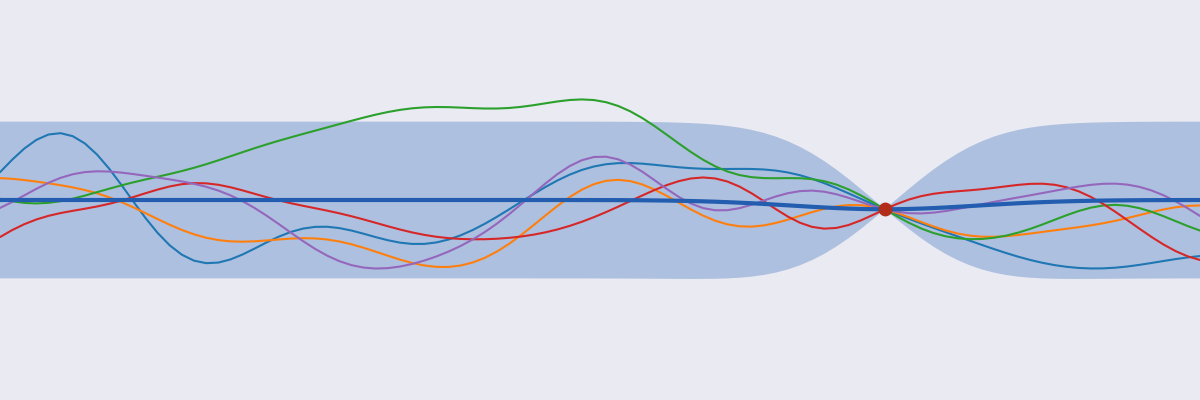
\includegraphics[width=\textwidth]{img_hyperopt/gp_posterior_1_point}
    \end{subfigure}

    \begin{subfigure}[b]{\textwidth}
        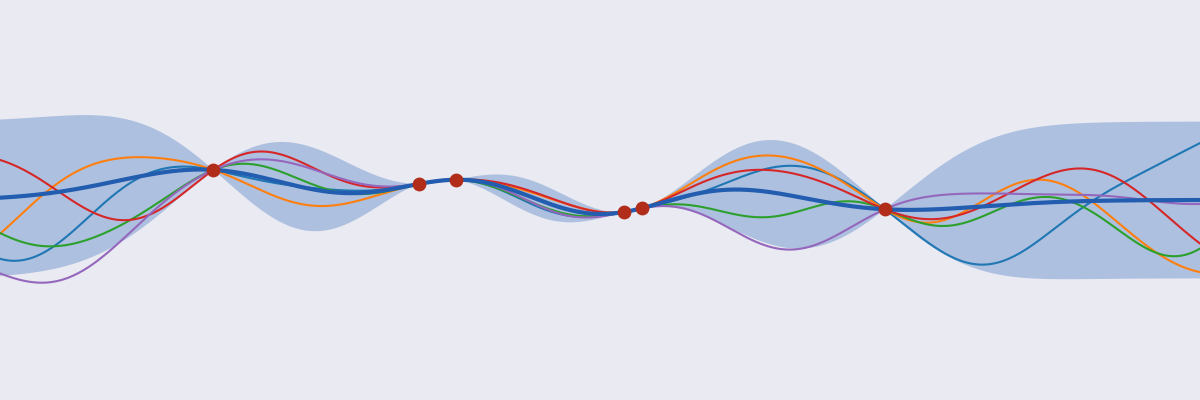
\includegraphics[width=\textwidth]{img_hyperopt/gp_posterior_6_point}
    \end{subfigure}
    \caption{Gaussian process posterior after fitting one point on top, six on the bottom. All the samples pass through those points and the variance is lower close to them.}
    \label{fig:gp_posterior}
\end{figure}

Figure~\ref{fig:gp_posterior} shows how samples from this distribution look like on a one dimensional problem. Each sample must go through every observed point, and the closer the points are, the less freedom the samples have to change. Outside of the range of observed points, the distribution quickly reverts to its prior. 

%So far we have assumed for simplification that the data is noise-free, however it is important to note that Gaussian processes are particularly well-adapted for dealing with noisy data. See~\textcite{rasmussen2005} for the changes to the equations.

\subsubsection{Kernels}

The most common kernel is the squared exponential kernel:
\begin{equation}
	k(\mathrm{x}, \mathrm{x'}) = \sigma^2 \exp\left( -\frac{||\mathrm{x} - \mathrm{x'}||_2^2}{2l^2}\right)
	\label{eq:sqexp}
\end{equation}
With this kernel, the influence of a point on the value of another point decays exponentially with their relative distance. This implies that the Gaussian process quickly reverts to its prior in areas without observed points.

This kernel has two hyper-parameters $\theta = \{ \sigma^2 , l \}$. $\sigma^2$ controls the scale of the predicted output and $l$ is a vector of same dimensionality as $\mathrm{x}$ called the characteristic length-scale which measures how much a change along each dimension affects the output. A low value means that a small change in the input results in a big change in the output, as shown in Figure~\ref{fig:gp_lengthscale}. 

\begin{figure}[htb]
    \centering
    \begin{subfigure}[b]{\textwidth}
        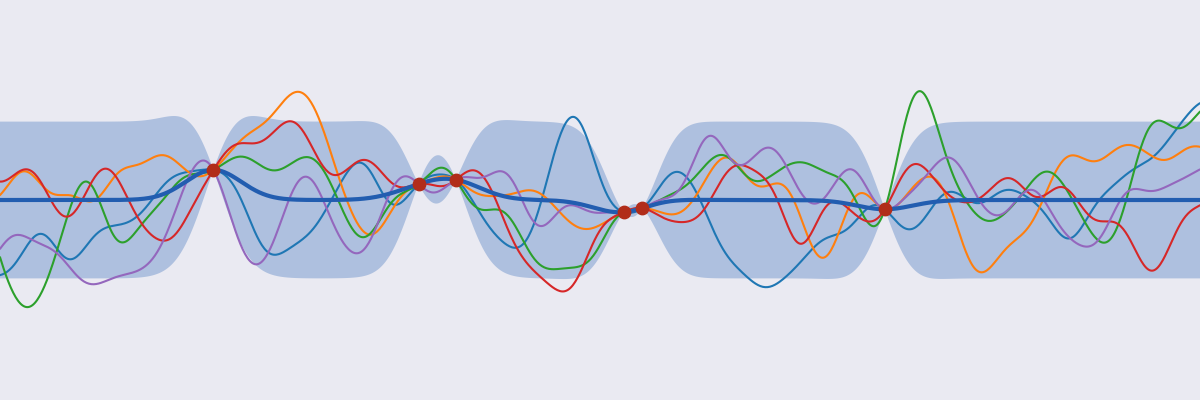
\includegraphics[width=\textwidth]{img_hyperopt/gp_lengthscale_small}
        \caption{$l = 0.3$}
    \end{subfigure}

    \begin{subfigure}[b]{\textwidth}
        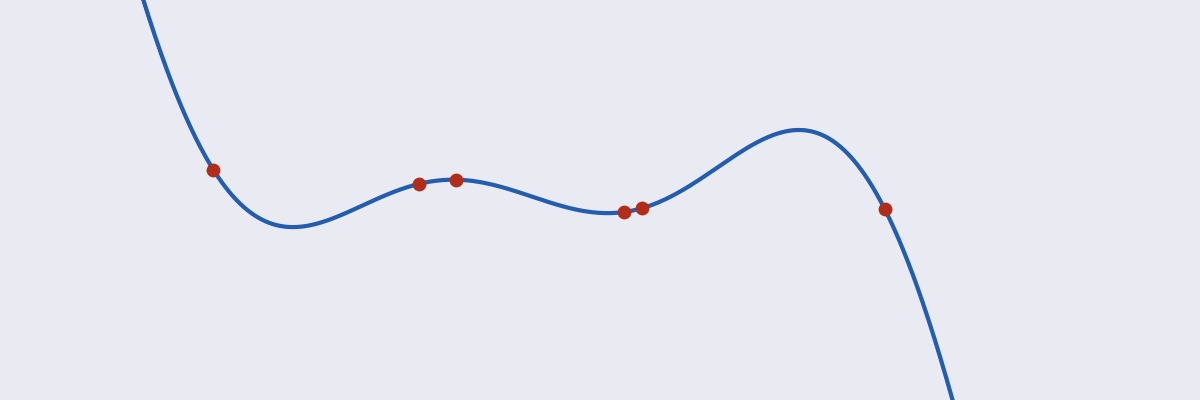
\includegraphics[width=\textwidth]{img_hyperopt/gp_lengthscale_big}
        \caption{$l = 3$}
    \end{subfigure}
    \caption{Gaussian process posterior after six points with different length-scale. On the top with a low length-scale, data points are almost irrelevant, the Gaussian process returns to its prior almost immediately. On the bottom, the GP has a very high confidence in its prediction.}
    \label{fig:gp_lengthscale}
\end{figure}

The squared exponential kernel is a special case of the Matérn family of covariance functions which are, noting $r = || \mathrm{x} - \mathrm{x'} ||_2$ defined as follows:
\begin{equation}
    k_{\nu}(r) = \sigma^2 \frac{2^{1-\nu}}{\Gamma(\nu)} \left( \sqrt{2\nu} \frac{r}{l}\right)^{\nu} B_{\nu} \left( \sqrt{2\nu} \frac{r}{l}\right)
\end{equation}
$\Gamma$ is the gamma function and $B_{\nu}$ is the modified Bessel function of the second kind. The hyper-parameters $\sigma^2$ and $l$ are the same as for the squared exponential kernel and $\nu$ is a measure of how smooth the function is. $\nu = 1/2$ results in a very rough function while $\nu \to \infty$ is the squared exponential kernel.

The samples from the squared exponential kernel are very smooth, and are in fact infinitely differentiable. This is usually too unrealistic for the process we are modelling. In the context of Bayesian optimization, a more realistic alternative is the Matérn $5/2$ kernel:
\begin{equation}
    k(r) = \sigma^2 \left( 1 + \frac{\sqrt{5}r}{l} + \frac{5r^2}{3l^2} \right) \exp \left( - \frac{\sqrt{5}r}{l}\right)
\end{equation}
The chosen value of $\nu = 5/2$ means that the samples will be twice differentiable, which is a good compromise between too smooth and too difficult to optimize $\theta$, as many point estimate methods require twice differentiability (\textcite{snoek2012NIPS}). Figure~\ref{fig:gp_matern} shows what samples from these kernels look like.

\begin{figure}[htb]
    \centering
    \begin{subfigure}[b]{\textwidth}
        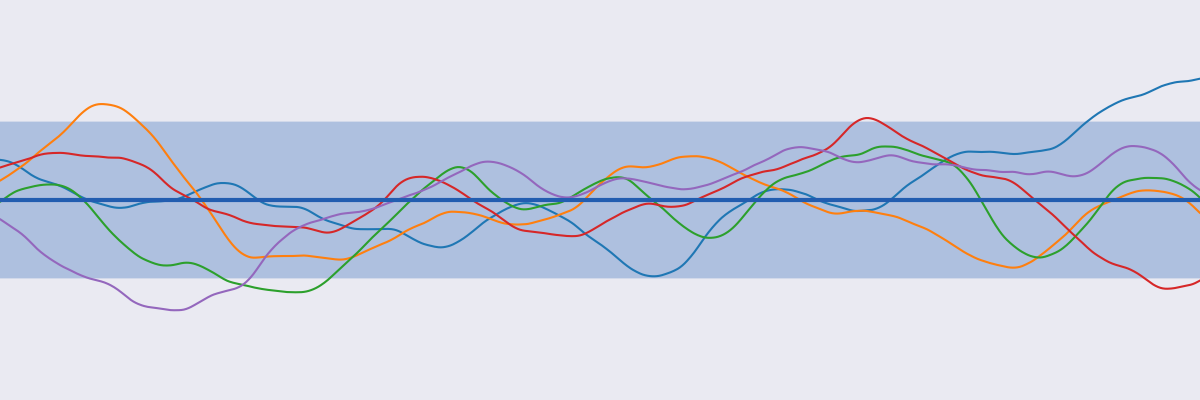
\includegraphics[width=\textwidth]{img_hyperopt/gp_matern_prior}
    \end{subfigure}

    \begin{subfigure}[b]{\textwidth}
        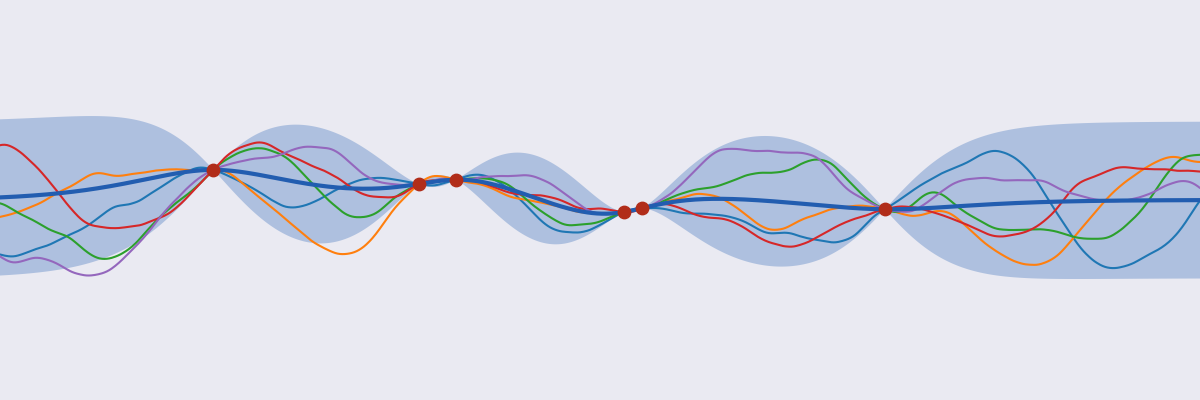
\includegraphics[width=\textwidth]{img_hyperopt/gp_matern_posterior}
    \end{subfigure}
    \caption{Gaussian process using a Matérn $5/2$ kernel. On the top, the prior. On the bottom, the posterior after fitting six points.}
    \label{fig:gp_matern}
\end{figure}

The presented kernels have the common property of being stationary, i.e they depend only of $\mathrm{x} - \mathrm{x'}$. They are invariant to translation. It is particularly relevant in the context of hyper-parameter optimization as the kernels make no difference between values of 3 and 2 or 1000 and 999. For hyper-parameters where such a difference matters should use a non-stationary kernel instead of the ones presented above (see~\textcite{paciorek2003NIPS}).

\subsubsection{Learning the kernel hyper-parameters}

Kernels have themselves hyper-parameters $\theta$ which need to be chosen. For example, the squared exponential kernel has $l$, the characteristic length-scale. As shown by~\textcite{neal1996phd}, the inverse of the length-scale determines how relevant an input is. In the context of hyper-parameter optimization, it can help to choose which hyper-parameters to tune carefully. It is therefore very important to select a good value for $l$. 

There are two ways to learn $\theta$. The first way is to maximize the marginal likelihood, which can be derived as:  
\begin{equation}
	\log p\left(\mathrm{y} | \mathrm{X}, \theta \right) = - \frac{1}{2} \mathrm{y}^T K^{-1} \mathrm{y} - \frac{1}{2} \log |K| - \frac{n}{2} \log 2 \pi
\end{equation}
The optimization can be done with any off-the-shelf method, eventually with multiple restarts as there are no guarantee of a unique optimum. 
%For example, the scikit-learn (\textcite{pedregosa2011sklearn}) implementation uses BFGS with 10 restarts by default.

The other solution is to not learn $\theta$ at all and instead marginalize the hyper-parameters, i.e. at the inference step compute:
\begin{equation}
    p\left( \mathrm{y_*} | \mathrm{X_*}, \mathrm{X}, \mathrm{y} \right)
    = \int p\left( \mathrm{y_*} | \mathrm{X_*}, \mathrm{X}, \mathrm{y}, \theta \right) p \left( \theta | \mathrm{X}, \mathrm{y} \right) d\theta
\end{equation}
This integral is usually intractable but can be approximated by sampling methods. \textcite{murray2010NIPS} use slice sampling, \textcite{garbuno2016CSDA} use asymptotically independent Markov sampling and \textcite{titsias2011} review different Monte Carlo methods used for this problem.

%%%%%%%%%%%%%%%%%%%%%%%%%%%%%%%%%%
\subsection{Acquisition functions}
\label{ssec:acqfunc}

In the context of Bayesian optimization, the Gaussian process gives for each set of hyper-parameters an estimation of the performance of the corresponding model and the uncertainty of the Gaussian process in its estimation. But we do not have a way to decide which model is the most interesting to train. Do we pick a model that will be slightly better than our best current model, i.e. where the Gaussian process gives low uncertainty, or do we pick a model with high uncertainty but which could have low performance? There is an exploration/exploitation trade-off to be found. It is the role of the acquisition function to determine which model to train.

The oldest acquisition function is the Probability of Improvement (\textcite{kushner1964}). It chooses the model which has the highest probability of having better results than a target, which is usually picked to be the loss of the current best model. The \textit{PI} is defined as below, where $\Phi$ is the Normal cumulative distribution function, $\mathrm{x}$ represents a given set of hyper-parameters, $y_*$ is the minimum loss found so far, $\mu$ is the mean returned by the Gaussian process and $\sigma$ the variance:
\begin{equation}
    PI(\mathrm{x}) = \Phi \left( \frac{y_* - \mu(\mathrm{x})}{\sigma(\mathrm{x})}\right)
\end{equation}
The problem with this function is that it is highly sensitive to the choice of target. The simplest choice is the minimum loss found so far, but the \textit{PI} will then sample models very close to the corresponding model completely ignoring exploration. A better target is how much to improve the minimum loss. But this choice is very inconvenient because we usually have no idea of how much better the performance can get. Should we try to find a model $1 \%$ better? $5 \%$? $25 \%$? If we pick too big an improvement, the function will simply select the models with the highest uncertainty.

Instead, we can use the Expected Improvement function (\textcite{schonlau1998},~\textcite{jones2001}) which builds on the Probability of Improvement as below where $\phi$ is the normal density function:
\begin{equation}
	EI(\mathrm{x})  = \sigma (\mathrm{x}) [u\Phi(u)+\phi(u)]
\end{equation}
with
\begin{equation}
	u = \frac{y_* - \mu(\mathrm{x})}{\sigma(\mathrm{x})}
\end{equation}
The Expected Improvement \textit{EI} is obtained by taking the expectation of the improvement function (\textcite{shahriari2016IEEE}), defined as:
\begin{equation}
	I(\mathrm{x}) = \left(y_* - \mu(\mathrm{x}) \right) \mathds{1} \left(y_* > \mu(\mathrm{x}) \right)
\end{equation}
This function is equal to $0$ if the predicted mean is less than the best loss found so far (which means that there is no improvement), otherwise it is proportional to the gap between the predicted mean and best loss. 

The Expected Improvement has a major advantage over the Probability of Improvement. The target is always the minimum loss found so far, meaning that there is no need to guess a threshold of improvement. 

%%%%%%%%%%%%%%%%%%%%%%%%%%%%%%%%%%
\subsection{Bayesian optimization algorithm}

In summary, Bayesian Optimization works as follows. Given a set of explored combinations and their associated models performance, a Gaussian process fitted on that set is used to predict the performance of untested combinations. Then, an acquisition function takes those predictions and decides which combination should be tested next. This combination is tested, added to the set of explored combinations, and the process is repeated as long as resources are available. This process can be seen in Figure~\ref{fig:bo} on a one-dimensional problem. 

\begin{figure}[htb]
	\centering
	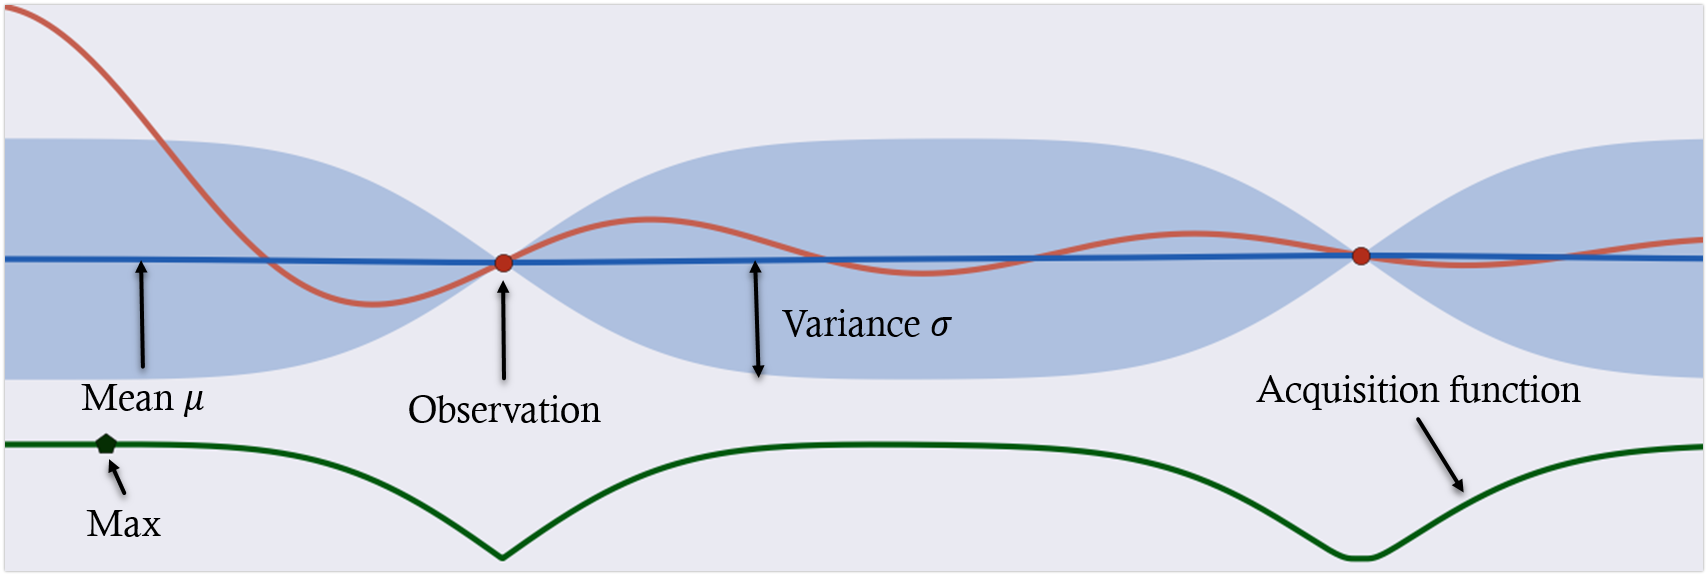
\includegraphics[width=\linewidth]{img_hyperopt/bo.png}
	\caption{Bayesian Optimization on a one dimensional function. The orange curve is the true loss function, the blue one is the prediction of the Gaussian process. The green curve is the acquisition function. The next evaluation will be at the maximum of the green curve.}
	\label{fig:bo}
\end{figure}

%The process can be initiated by choosing the first model randomly or from a hand-crafted baseline when available.

%Some questions remain. How to pick the first model ? Select a random configuration of hyper-parameters from the hyper-parameter space. Should the Gaussian process predict the loss on the training set or on the validation set ? The loss on the validation set is to be preferred. How to sample configurations ? Uniformly from the hyper-parameter space. How many configurations should be sampled before selecting a model to train ? As many as reasonably possible. The step of selecting a model should be much faster than training it, and most of the cost of Bayesian optimization should be in the inversion of the Gram matrix (see Section~\ref{ssec:practical} for details).

%Hyperopt~\textcite{bergstra2013ICML}

%Practical~\textcite{snoek2012NIPS}

%%%%%%%%%%%%%%%%%%%%%%%%%%%%%%%%%%
% \subsection{Practical Challenges}
% \label{ssec:practical}

% %==One important aspect of this method is that the training time of the model is a dimension of the hyper-parameter space. This means that the method is free to choose how long to train each model. In practice we found that it prefers longer training time, even though it looks like a lower training time is enough to get a good estimate of the worth of the model and would allow the evaluation of more models. This is a flaw of the method, which lacks an explicit notion of budget and a way to best exploit it.

% \subsubsection{Conditional spaces}

% TODO
% \begin{itemize}
%     \item Describe cylindrical embeddings
%     \item Describe tree of Parzen estimator
% \end{itemize}

% The version of Bayesian optimization we presented deals efficiently with both discrete and continuous hyper-parameters. But what about conditional hyper-parameters ? For example, some hyper-parameters could be specific to a particular layer and one hyper-parameter could control the number of layers. But then, what happens to the hyper-parameters of a non-existent layer ? With a Gaussian process, we need to give them a value and it means there will be many configurations that corresponds to the same model. In practice, we can ignore those cases, and the Gaussian process will eventually give a low uncertainty in those regions and pick models elsewhere. But this is extremely wasteful as we will retrain the same model many times before this happens ! 

% One solution is to use a specialized kernel called a cylindrical kernel (\textcite{swersky2013},~\textcite{oh2018}).

% Another solution is to not use a Gaussian process at all. It has been our model of choice so far but other alternatives exist. One such alternative is tree-structured Parzen estimator (\textcite{bergstra2011NIPS}).

% \subsubsection{Parallelization}

% Open problem using GP

% See combination with Hyperband for a potential solution

% \subsubsection{Non-stationarity}
% \label{ssec:nosta}

% Input Warping~\textcite{snoek2014ICML}

% \subsubsection{Scaling}

% Doesn't work well in high-dimension or with thousands of data points

% Conditional neural processes ?

%%%%%%%%%%%%%%%%%%%%%%%%%%%%%%%%%%
\section{Incremental Cholesky decomposition}
\label{sec:cholesky}

\subsection{Motivation}
\label{ssec:motivation}

The costliest part of Bayesian optimization is the construction of the Gram matrix $K$ and the computation of its invert $K^{-1}$. To reduce that cost, the standard solution is to compute the Cholesky decomposition $L$ of the Gram matrix and invert the decomposition. Every time the Gram matrix is modified, the Cholesky decomposition and its inverse are fully recomputed.

However, Bayesian optimization alters the Gram matrix only by adding new rows and columns corresponding to the covariance between the $n$ older combinations and the $k$ new combinations. The Gram matrix can therefore be decomposed in blocks where one of them is the previous Gram matrix. By calling $K_{(n,n)}$ the previous matrix and $K_{(n+k,n+k)}$ the new one with the added points, the decomposition is:
\begin{equation}
	K_{(n+k,n+k)} = 
	\begin{pmatrix}
    K_{(n,n)} & K_{(k,n)}^T \\
    K_{(k,n)} & K_{(k,k)}
  \end{pmatrix}
\end{equation}
Likewise, the Cholesky decomposition and its inverse can also be decomposed into blocks where one is the previous Cholesky decomposition as we show in Section~\ref{ssec:formulas}. We then argue in Section~\ref{ssec:complexity} that this can be used to make Bayesian optimization faster by updating incrementally the Cholesky decomposition instead of fully recomputing it each time.

\subsection{Deriving the formulas}
\label{ssec:formulas}

Let us recall that the Cholesky decomposition $L_{(n)}$ of a positive definite matrix $K_{(n)}$ is a decomposition of the form:
\begin{equation}
	K_{(n)} = L_{(n)} L_{(n)}^T
\end{equation}
where $L_{(n)}$ is a lower triangular matrix. The decomposition is unique only if $K_{(n)}$ is positive definite. Since $K_{(n)}$ is a Gram matrix, it is always guaranteed to be positive semi-definite (i.e. $\forall v \in \mathbb{R}^n, \mkern10mu v^T K_{(n)} v \geq 0$), but if the rows and columns are unique (i.e. there are no duplicate data points), then it is positive definite.

\subsubsection[Formula for the Cholesky decomposition]{Formula for $L_{(n+k)}$}

When adding $k$ points to a Gram matrix of $n$ points, the block decomposition of the new Cholesky decomposition is:
\begin{alignat*}{2}
	&&L_{(n+k)} L_{(n+k)}^T &= K_{(n+k,n+k)} \\
	\Leftrightarrow\mkern40mu
	&&\begin{pmatrix}
    A & B \\
    C & D
  \end{pmatrix}
  \begin{pmatrix}
    A^T & C^T \\
    B^T & D^T
  \end{pmatrix} &= 
  \begin{pmatrix}
    K_{(n,n)} & K_{(k,n)}^T \\
    K_{(k,n)} & K_{(k,k)}
  \end{pmatrix}
\end{alignat*}
$B$ is obviously $0$ since a Cholesky decomposition is lower triangular.

By developing the block decomposition, we obtain the following equation for $A$:
\begin{equation*}
	A A^T + B B^T = A A^T = K_{(n,n)}
\end{equation*}
Since the Cholesky decomposition is unique, $A = L_{(n)}$. The equation for $C$ is also simple to solve:
\begin{alignat*}{2}
	&&C A^T + D B^T &= C L_{(n)}^T = K_{(k,n)} \\
	\Leftrightarrow\mkern40mu
	&&C &= K_{(k,n)} (L_{(n)}^T)^{-1}
\end{alignat*}
Solving for $D$ requires more work. Developing the block decomposition, we have:
\begin{alignat*}{2}
	&&C C^T + D D^T &= K_{(k,k)} \\
	\Leftrightarrow\mkern40mu
	&&D D^T &= K_{(k,k)} - K_{(k,n)} (K_{(n,n)})^{-1} K_{(k,n)}^T
\end{alignat*}
If we can show that $K_{(k,k)} - K_{(k,n)} (K_{(n,n)})^{-1} K_{(k,n)}^T$ is definite positive then $D$ is its unique Cholesky decomposition.

Let $w \in \mathbb{R}^{n+k} \quad \text{s.t.} \quad w = \begin{pmatrix}
    u \\
    v
  \end{pmatrix}, u \in \mathbb{R}^n, v \in \mathbb{R}^k$, we have $w^T K_{(n+k,n+k)} w \geq 0$ because $K_{(n+k,n+k)}$ is a Gram matrix. Using its block decomposition and developing it, we have:
\begin{alignat*}{2}
  &&\begin{pmatrix}
    u \\
    v
  \end{pmatrix} ^T
  \begin{pmatrix}
    K_{(n,n)} & K_{(k,n)}^T \\
    K_{(k,n)} & K_{(k,k)}
  \end{pmatrix}
  \begin{pmatrix}
    u \\
    v
  \end{pmatrix}
  &\geq 0 \\
  \Leftrightarrow\mkern40mu
  &&u^T K_{(n,n)} u + u^T K_{(k,n)}^T v +
  v^T K_{(k,n)} u + v^T K_{(k,k)} v
  &\geq 0 \\
  \Leftrightarrow\mkern40mu
  &&u^T K_{(n,n)} u + 
  2 u^T K_{(k,n)}^T v +
  v^T K_{(k,k)} v
  &\geq 0
\end{alignat*}
Using three successive change of variables, this equation becomes a second-order polynomial. The first change is $u = K_{(n,n)}^{-1} x$:
\begin{equation*}
  x^T (K_{(n,n)}^T)^{-1} x + 
  2 x^T (K_{(n,n)}^T)^{-1} K_{(k,n)}^T v +
  v^T K_{(k,k)} v
  \geq 0
\end{equation*}
The second change is $x = t y$ where $t$ is a scalar:
\begin{equation*}
  t^2 y^T (K_{(n,n)}^T)^{-1} y + 
  2 t y^T (K_{(n,n)}^T)^{-1} K_{(k,n)}^T v +
  v^T K_{(k,k)} v
  \geq 0
\end{equation*}
The final change is $y = K_{(k,n)}^T v$:
\begin{equation*}
  t^2 v^T K_{(k,n)} (K_{(n,n)}^T)^{-1} K_{(k,n)}^T v + 
  2 t v^T K_{(k,n)} (K_{(n,n)}^T)^{-1} K_{(k,n)}^T v +
  v^T K_{(k,k)} v
  \geq 0
\end{equation*}
The determinant of this polynomial verifies:
\begin{alignat*}{2}
  &&4 (v^T K_{(k,n)} (K_{(n,n)}^T)^{-1} K_{(k,n)}^T v)^2 &-
  4 (v^T K_{(k,n)} (K_{(n,n)}^T)^{-1} K_{(k,n)}^T v)
  (v^T K_{(k,k)} v)
  \leq 0 \\
  \Leftrightarrow\mkern20mu
  &&(v^T K_{(k,n)} (K_{(n,n)}^T)^{-1} K_{(k,n)}^T v)^2
  &\leq 
  (v^T K_{(k,n)} (K_{(n,n)}^T)^{-1} K_{(k,n)}^T v)
  (v^T K_{(k,k)} v)
\end{alignat*}
But $v^T K_{(k,k)} v \geq 0$ since $ K_{(k,k)}$ is a Gram matrix (i.e. positive semi-definite), meaning by necessity $v^T K_{(k,n)} (K_{(n,n)}^T)^{-1} K_{(k,n)}^T v \geq 0$ and $K_{(k,n)} (K_{(n,n)}^T)^{-1} K_{(k,n)}^T$ is positive semi-definite.

Therefore, $K_{(k,k)} - K_{(k,n)} (K_{(n,n)}^T)^{-1} K_{(k,n)}^T$ is positive semi-definite, it is positive definite as long as none of the $k$ new combinations are duplicates of the $n$ previous combinations and $D D^T$ is its Cholesky decomposition.
\begin{equation*}
  D = cho(K_{(k,k)} - K_{(k,n)} (K_{(n,n)}^T)^{-1} K_{(k,n)}^T) = L_{(k)}
\end{equation*}
The final formula for the incremental Cholesky decomposition is:
\begin{equation}
  L_{(n+k)} = 
  \begin{pmatrix}
    L_{(n)} & 0 \\
    K_{(k,n)} (L_{(n)}^T)^{-1} & L_{(k)}
  \end{pmatrix}
\end{equation}
Since this formula requires the costly computation of $L_{(n)}^{-1}$, we would also like to find an incremental formula for it.

\subsubsection[Formula for the inverse Cholesky decomposition]{Formula for $L_{(n+k)}^{-1}$}

A standard expression for the inversion of a block matrix is:
\begin{equation*}
  \begin{pmatrix}
    A & B \\
    C & D
  \end{pmatrix}^{-1} = 
  \begin{pmatrix}
    A^{-1} + A^{-1} B (D - C A^{-1} B)^{-1} C A^{-1} & - A^{-1} B (D - C A^{-1} B)^{-1} \\
    - (D - C A^{-1} B)^{-1} C A^{-1} & (D - C A^{-1} B)^{-1}
  \end{pmatrix}
\end{equation*}
Simplifying with $L_{(n+k)}$ found previously, we have:
\begin{equation}
  L_{(n+k)}^{-1} =
  \begin{pmatrix}
    L_{(n)} & 0 \\
    K_{(k,n)} (L_{(n)}^T)^{-1} & L_{(k)}
  \end{pmatrix}^{-1} = 
  \begin{pmatrix}
    L_{(n)}^{-1} & 0 \\
    - L_{(k)}^{-1} K_{(k,n)} (L_{(n)}^T)^{-1} L_{(n)}^{-1} & L_{(k)}^{-1}
  \end{pmatrix}
\end{equation}

\subsection{Complexity improvement}
\label{ssec:complexity}

A standard Cholesky decomposition has a complexity of $O \left( (n + k)^3 \right)$ with $n + k$ the number of observed combinations. With our formulas, since we already have $L_{(n)}$, all that is left is to compute $L_{(k)}$, which has a cost of $O \left( k^3 \right)$. Since Bayesian optimization is called after every tested combination, $k = 1$, the Gram matrix just has one new row and one new column. $L_{(k)}$ and its inverse are trivial to compute.

There is however an increased cost in memory, as $L_{(n)}$ and $L_{(n)}^{-1}$ must be stored between calls of Bayesian optimization. They are two $n \times n$ triangular matrices, storing them cost $O \left( n^2 \right)$, which seems a reasonable price to pay for the performance improvement.

%%%%%%%%%%%%%%%%%%%%%%%%%%%%%%%%%%%%%%%%%%%%%%%%%%%%%%%%%%%%%%%%%%%%%%%%%%%%%%%%%%%%%%%%%%%%%%%
\section{Comparing Random Search and Bayesian Optimization}
\label{sec:compare}

In this section we study the theoretical performance of random search, before devising an experiment that compares the performance of random search and Bayesian optimization in a practical setting.

%%%%%%%%%%%%%%%%%%%%%%%%%%%%%%%%%%
\subsection{Random search efficiency}
\label{ssec:random}

How many models of a hyper-parameters space should be trained in order to be reasonably certain to have trained one of the best models? If we knew the loss $l_{min}$ of the best model, how long would it take to find a model with a loss such that $l \leq (1 + \alpha) l_{min}$? Due to the relative simplicity of random search, we can derive theoretical bounds to answer these questions.

Let $N$ be the total number of models in the hyper-parameters space, $M$ the number of models satisfying our performance criteria (alternatively, the $M$ best models of the space) and $n$ the number of models to train.

Considering that random search chooses models uniformly, the probability of drawing one of the best models the first time is simply $\frac{M}{N}$. The second time, it is $\frac{M}{N - 1}$ since we do not allow redrawing a model. We can therefore define the probability of not drawing any satisfying models after $n$ draws as the following equation, where $Y$ is the random variable of failing to draw an acceptable models among $n$ draws in a row.
\begin{equation}
    P \left( Y = n \right) = \prod_{k = 0}^{n} \left( 1 -  \frac{M}{N - k} \right)
\end{equation}
This is a particular case of the hypergeometric distribution. From there, the probability of drawing an acceptable model at the $n$-th draw is:
\begin{equation}
    P\left(X = n \right) = \frac{M}{N - n} \prod_{k = 0}^{n - 1} \left( 1 -  \frac{M}{N - k} \right)
\end{equation}
$X$ is the random variable of drawing an acceptable model after $n - 1$ bad draws. The probability of drawing an acceptable model in the first $n$ draws is:
\begin{equation}
    P\left(X \leq n \right) = \sum_{k = 0}^{n} P\left(X = k \right)
\end{equation}
From this equation we can compute the number of draws required to have drawn a model in the top $\alpha \%$, by setting $M$ as a fraction of $N$. Moreover since the equation depends only of the ratio $\frac{M}{N - k}$, the effect of $k$ becomes negligible as $N$ grows bigger and the equation converges.

\begin{table}[htb]
	\centering
	\begin{tabular}{ | l | c | c | c | }
		\hline
		 & $p > 0.5$ & $p > 0.95$ & $p > 0.99$ \\ 
		\hline
		Top $1 \%$ & 69 & 298 & 458 \\
		Top $5 \%$ & 14 & 59 & 90 \\
		Top $10 \%$ & 7 & 29 & 44 \\
		\hline
	\end{tabular}
	\caption{Number of draws required to have drawn a model in the top $\alpha \%$ with probability $p$ in a space of 100 000 combinations.}
	\label{table:random_search_bounds}
\end{table}

In Table~\ref{table:random_search_bounds}, we present some of those results, which allow us to draw the following strong conclusion. For any hyper-parameter space, random search will draw a model in the top $5 \%$ of models in 90 draws with a probability of $99 \%$. Less than a hundred draws is sufficient to draw one of the best models of any hyper-parameter space. It is a surprisingly low number given the simplicity of the method.

However that is only one of the questions we asked. Ranking the models by their performance does not guarantee that a model in the top $\alpha \%$ is within $\alpha \%$ of the performance of the best model, unless model performance happens to be uniformly distributed. Since we have no idea of how model performance is distributed, we cannot go further in our theoretical analysis. In Section~\ref{ssec:cifar_analysis}, we return to this question by studying empirically the distribution of model performance.

%%%%%%%%%%%%%%%%%%%%%%%%%%%%%%%%%%
\subsection{Bayesian optimization efficiency}

While we were not able to obtain similar results for Bayesian optimization as we did for random search, we expose some of the difficulties in doing so.

First any analysis depends of the exact setup of Bayesian optimization. A change of kernel or acquisition function changes the results. But the main problem is that, because the process learns the structure of the hyper-parameter space, any analysis would need to work in a particular space.

None of those difficulties prevent us from measuring the empirical performance of Bayesian optimization, as we show in the next section.

%%%%%%%%%%%%%%%%%%%%%%%%%%%%%%%%%%
\subsection{Experiments on CIFAR-10}
\label{ssec:cifar_analysis}

\subsubsection{Setup}

In order to compare the performance of the different hyper-parameter optimization methods, we devised a hyper-parameter space containing 600 models and trained them all on the CIFAR-10 dataset (\textcite{krizhevsky2009}).

The dataset is composed of 60 000 images equally divided in 10 classes. The images are 32x32 RGB images. The training set contains 50 000 images, the test set 10 000.

Since the goal of the experiment is not to beat the state-of-the-art on the dataset, the selected hyper-parameter space and the resulting models are small and simple. Each model is trained for a total of 10 minutes on a NVIDIA TITAN X card. 

We then compare in which order the different methods selected the models. The methods are evaluated on the time needed to select the best model, as well as the time needed to select a model in the top $\alpha \%$.
%but also on the average performance of the selected models, i.e. if we rank the models by their performance, how close was each method from selecting the models in that order.

However one run is not enough to conclude that Bayesian optimization on average is more efficient than random search. Due to the huge computing cost, we cannot do hundreds of runs with different seeds and retrain each network every time. But if we do not retrain the network but change the seeds of the search policy, we can simulate hundreds of runs at a low cost. 

There are a total of $600!$ way to explore this space, but because we do not retrain the models, all the randomness in Bayesian optimization is in the choice of the first model, leaving us with only 600 possible paths through this space. We computed them all, then randomly selected 600 ordering for random search.

\subsubsection{Models distribution}

\begin{figure}[htb]
	\centering
	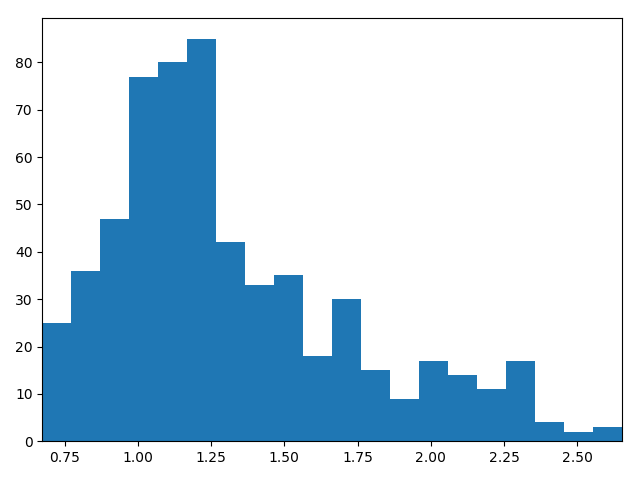
\includegraphics[width=0.7\linewidth]{img_hyperopt/cifar_hist.png}
	\caption{Distribution of the models performance.}
	\label{fig:cifar_hist}
\end{figure}

Before comparing the search methods, we look at the distribution of models performance in Figure~\ref{fig:cifar_hist}. A few models are really good, most are average and then there is a long trail of progressively worse models. It looks like a skew normal distribution. 

We cannot extrapolate that every hyper-parameter space will have a distribution like this, but we assume for now that this is the case for hyper-parameter spaces designed in practice.

Since the distribution is not uniform, there is a difference between models in the top $5 \%$ of models and models that have a performance within $5 \%$ of the performance of the best model. In this case, there are 30 models in the top $5 \%$ of models (since there are 600 models), but only 6 are within $5 \%$ of the performance of the best model. In this case, the 30-th best model is within $18 \%$ of the best model.

This distinction is important because it changes our evaluation of the methods. We are not simply interested in the average time to find a model in the top $\alpha \%$ of models, but also in the average time to find a model within $\alpha \%$ of the best model.

\subsubsection{Results}

\begin{figure}[htbp]
	\begin{subfigure}[b]{\textwidth}
            \centering
            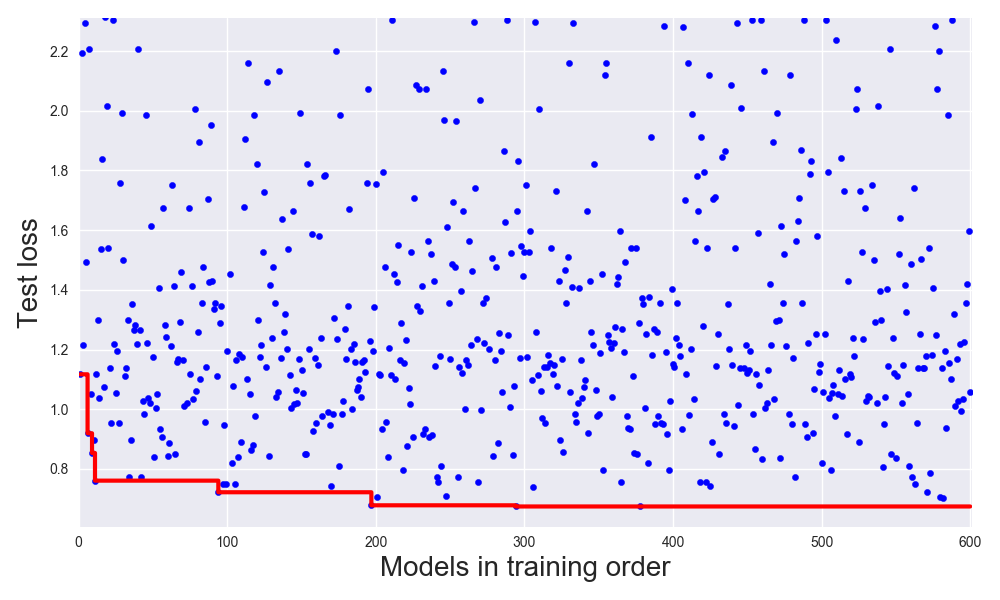
\includegraphics[width=\linewidth]{img_hyperopt/cifar_random}
    \end{subfigure}%
    
    \begin{subfigure}[b]{\textwidth}
            \centering
            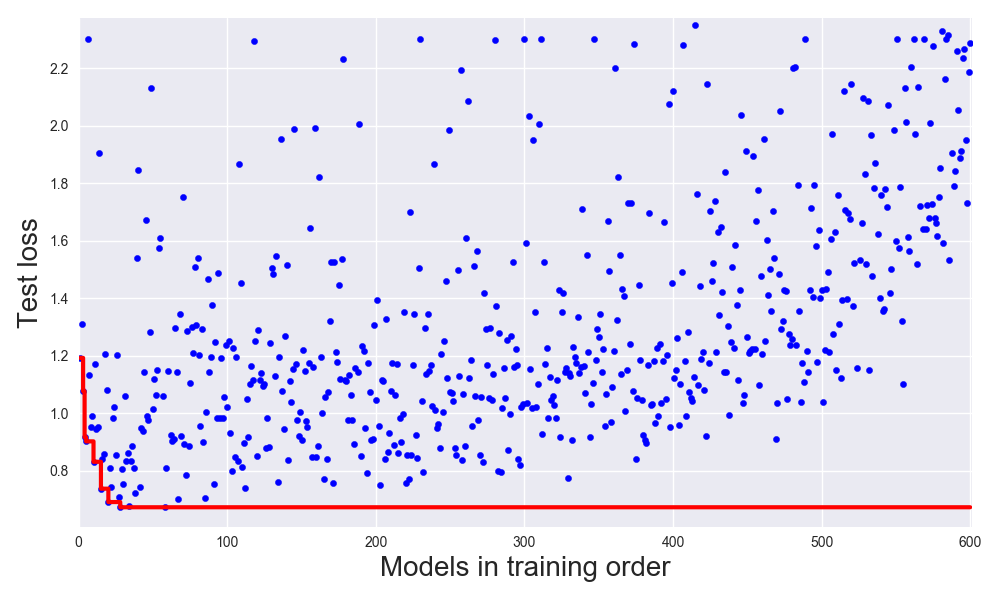
\includegraphics[width=\linewidth]{img_hyperopt/cifar_bo}
    \end{subfigure}%
    \caption{Comparing the model order chosen by random search (top) vs Bayesian optimization (bottom).}
	\label{fig:cifar_loss}
\end{figure}

First, we look at the order in which models where selected during one run, shown in Figure~\ref{fig:cifar_loss}. The blue points represent the test loss of the models in the order the methods selected them, and the red line shows the minimum loss found at a given time. There is a clear trend present for Bayesian optimization where the combinations evaluated later have low performance, suggesting it did learn to predict correctly the performance of untested combination. In this run, it was also able to find the best model much earlier than random search. Random search behaves as expected and models performance is uniformly distributed.

\begin{table}[htb]
	\centering
	\begin{tabular}{ | l | c | c | c | c | }
		\hline
		 & \multicolumn{2}{|c|}{Random Search} & \multicolumn{2}{|c|}{Bayesian optimization} \\ 
		%\hline
		& Average & Worst & Average & Worst \\
		\hline
		Best model & $297 \pm 171$ & $599$ & $87 \pm 64$ & $249$ \\
		\hline
		Within $1 \%$ & $146 \pm 114$ & $554$ & $26 \pm 16$ & $120$ \\
		Within $5 \%$ & $87 \pm 75$ & $397$ & $17 \pm 11$ & $67$ \\
		Within $10 \%$ & $54 \pm 52$ & $296$ & $15 \pm 9$ & $44$ \\
		\hline
		Top $1 \%$ & $87 \pm 75$ & $397$ & $17 \pm 11$ & $67$ \\
		Top $5 \%$ & $18 \pm 17$ & $106$ & $10 \pm 8$ & $38$ \\
		Top $10 \%$ & $10 \pm 10$ & $62$ & $7 \pm 7$ & $36$ \\
		\hline
	\end{tabular}
	\caption{Average and worst number of draws taken by each method to reach different goals over 600 runs. Within $\alpha \%$ mean within $\alpha \%$ of the performance of the best model.}
	\label{table:search_average}
\end{table}

To confirm these trends, we look at the average number of draws taken by each method to reach different goals (Table~\ref{table:search_average}).

Random search needed on average 297 draws before finding the best model, which is within the expected range of the theoretical value of 300 draws. If we rank the model by their performance, random search needed an average of 18 draws to find a model in the top $5\%$ and 87 to find a model in the top $1\%$.

In comparison, Bayesian optimization did a lot better on every goal. On average it needed 87 draws to find the best model and only 17 to find a model in the top $1 \%$. In most cases the worst run of Bayesian optimization performed better than the average run of random search.

\begin{figure}[htb]
	\centering
	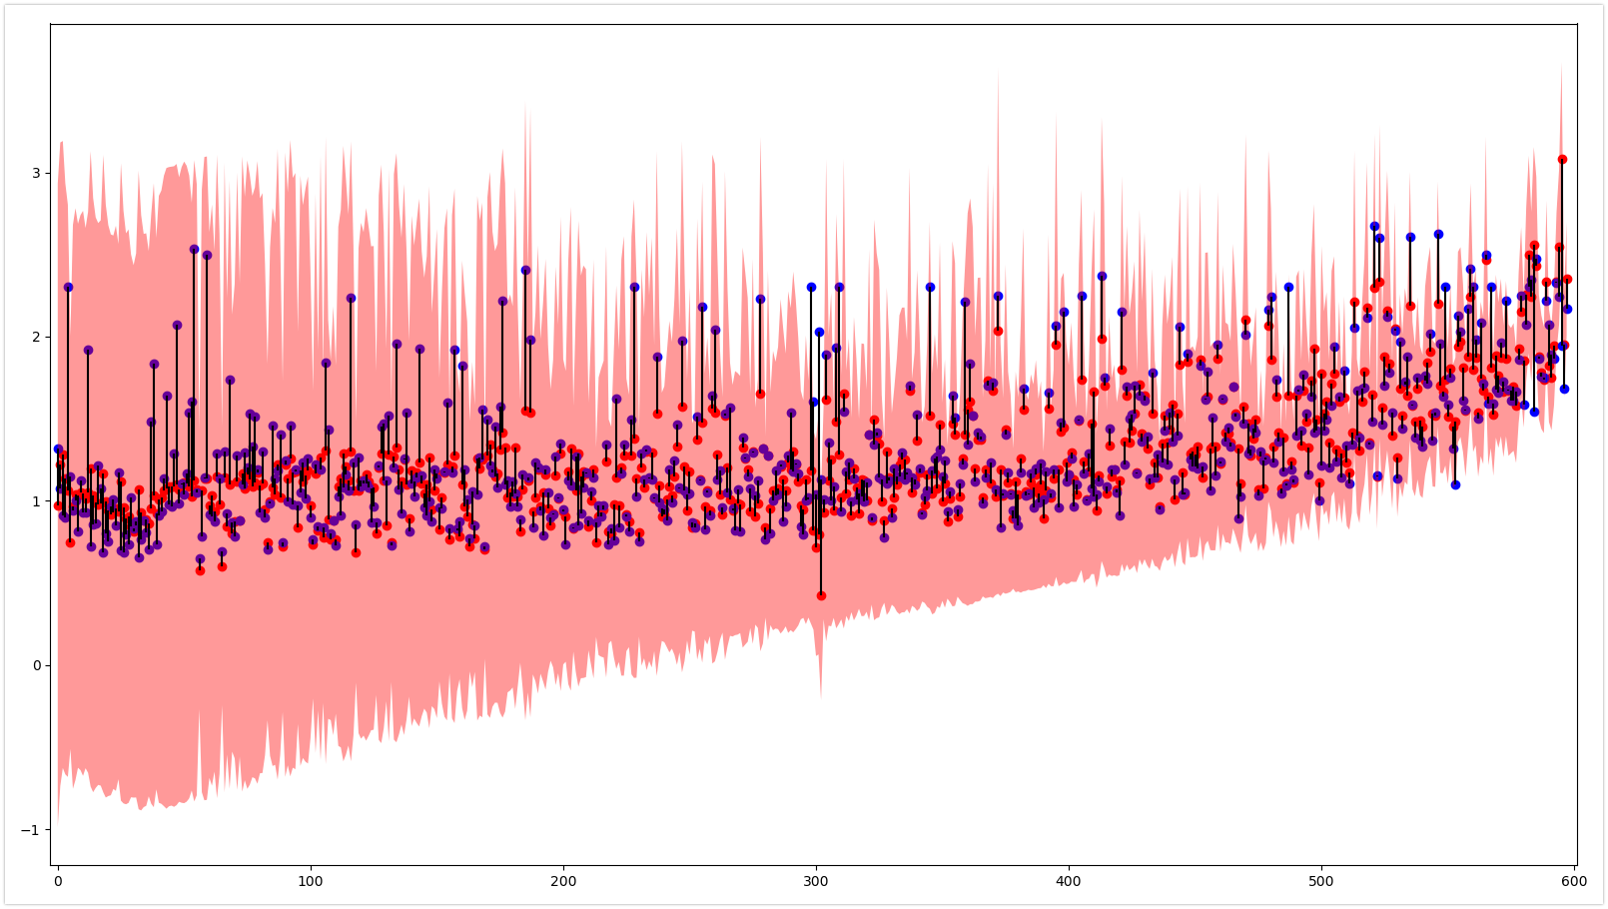
\includegraphics[width=\linewidth]{img_hyperopt/bo_error_time.png}
	\caption{Model performance predicted by the Gaussian process in red vs the true performance in blue. The colored area is the $95 \%$ prediction interval.}
	\label{fig:bo_error_time}
\end{figure}

To confirm whether the Gaussian process is learning the structure of the hyper-parameter space, Figure~\ref{fig:bo_error_time} shows the predicted performance and the true performance, as well as the $95 \%$ prediction interval. As more models are used to refine the Gaussian process, the prediction interval shrinks, i.e. the Gaussian process becomes more confident in its prediction. Prediction for outliers, in this case models that do not learn, is highly inaccurate at the beginning and is still the main source of error at the end.

\subsection{Conclusion}

We designed an experiment to measure and compare the performance of random search and Bayesian optimization on a setting mimicking real life usage. Performance of random search matched closely theoretical results, showing the surprising efficiency of this method. Bayesian optimization outperformed random search on every metric, which justifies its much higher implementation cost.

Analysis of the models performance suggested that it is normally distributed, but testing on other tasks with other hyper-parameter spaces is required. Likewise, while we expect Bayesian optimization to always outperform random search, further confirmation is required.

%%%%%%%%%%%%%%%%%%%%%%%%%%%%%%%%%%%%%%%%%%%%%%%%%%%%%%%%%%%%%%%%%%%%%%%%%%%%%%%%%%%%%%%%%%%%%%%
\section{Combining Bayesian Optimization and Hyperband}
\label{sec:cap}

This section describes and extends work that was presented at CAp 2017 (\textcite{bertrand2017CAp}).

%%%%%%%%%%%%%%%%%%%%%%%%%%%%%%%%%%
\subsection{Hyperband}
\label{ssec:hyperband}

A property of neural networks is that their training is iterative, usually some variant of gradient descent. A consequence is that it is possible to interrupt training at any time, evaluate the network, then resume training. This is the property Hyperband (\textcite{li2017ICLR}) takes advantage of.

The principle is simple: pick randomly a group of configurations from a uniform distribution, train the corresponding networks partially, evaluate them, resume training of the most performing ones, and so on until a handful of them have been trained to completion. Then pick a new group and repeat the cycle until exhaustion of the available resources.

But a problem appears: at which point in the training can we start evaluating the models? Too soon and they will not have started to converge, making the evaluation meaningless, too late and we have wasted precious resources training under-performing models. Moreover, we do not know how to find that point and it changes between tasks. Hyperband's answer is to divide a cycle into brackets. Each bracket has the same quantity of resource at its disposal. The difference between brackets is the point at which they start evaluating the models. The first bracket will start evaluating and discarding models very early, allowing it to test a bigger number of configurations, while the last bracket will test only a small number of configurations but will train them until the end.

The algorithm is controlled by two hyper-parameters: the maximal quantity of resources $R$ that can be allocated to a given model, and the proportion of configurations $\eta$ kept at each evaluation.

%%%%%%%%%%%%%%%%%%%%%%%%%%%%%%%%%%
\subsection{Combining the methods}

Bayesian optimization and Hyperband being orthogonal approaches, it seems natural to combine them. Hyperband chooses the configurations to train uniformly and intervenes only during training. On the other side, Bayesian optimization picks configurations carefully by modelling the loss function, then let them train without interruption.

As a result, Hyperband does not improve the quality of its selection with time, while Bayesian optimization regularly loose time training bad models.

Combining the methods fixes those problems. Model selection is done by Bayesian optimization as described in Section~\ref{sec:bo}, then Hyperband train them as described in Section~\ref{ssec:hyperband}. Two changes are required for Bayesian optimization, as it needs some way to distinguish between fully-trained models and partially trained models. To do that, the training time becomes an hyper-parameter, making the performance of each model at every minute a distinct point. The performance prediction is then done at the training time corresponding to Hyperband's first evaluation, to have only one prediction per model.

The second change is to normalize the values returned by the acquisition function to make it a probability distribution. In the standard usage of Bayesian optimization, the chosen model is the argmax of the acquisition function. Choosing the top x models yield models that are very close as the acquisition function is smooth and gives similar values for nearby combinations. This strategy removes the property of Hyperband to explore many regions of space at the same time. Normalizing the values and drawing from this distribution keeps this property, while making the selection smarter over time as it changes to reflect the knowledge acquired from the trained models.

The proposed algorithm is as follows: the first group of configurations is chosen randomly and evaluated according to Hyperband. All subsequent selections are done by training a Gaussian process with a squared-exponential kernel on all evaluated models. The expected improvement is then computed on all untested combinations and normalized to make a probability distribution from which the next group of models is sampled.

%%%%%%%%%%%%%%%%%%%%%%%%%%%%%%%%%%
\subsection{Experiments and results}

We compare the three methods presented above: Bayesian optimization, Hyperband, and Hyperband using Bayesian optimization. The algorithms were implemented in Python using scikit-learn~\textcite{pedregosa2011sklearn} for the Gaussian processes and Keras~\textcite{chollet2015keras} as the deep learning framework.

Comparison was done on the CIFAR-10 dataset~\textcite{krizhevsky2009}, which is a classification task on $32 \times 32$ images. The image set was split 50\% for the training set used to train the neural networks, 30\% for the validation set used for the Bayesian model selection and the rest as test set used for the reported results below. 

Each method is allocated a total budget $B = 4000$ minutes that it is free to allocate however it wants. The choice of having a budget in time means that models will not be trained in epoch as is the most common, but in minutes. This is a practical choice that allows to estimate accurately the total time that the search takes, though it has the effect of favouring small networks. Indeed, two models trained an equal amount of time will not have seen an equal amount of data if one model is bigger and thus slower than the other. The choice to constrain in time instead of epoch means that the quantity of data seen by the models depends on the GPU. The training is done on two NVIDIA TITAN X.

The chosen architecture is a standard convolutional neural network with varying number of layers, number of filters and filter size per layer. Other hyper-parameters involved in the training method are: the learning rate, the batch size and the presence of data augmentation. In the end there is 6 hyper-parameters to tune for a total of 19 200 possible configurations.

For Hyperband, we chose $R = 27$, meaning 27 models are chosen at each iteration and are trained for a maximum of 27 minutes, and $\eta = 3$ which means that $1/3$ of the models are kept at each evaluation. In the case of Bayesian optimization, each model was trained a full $30$ minutes but they are chosen sequentially.

\begin{figure}[htb]
	\begin{minipage}[b]{.49\linewidth}
		\centering
		\centerline{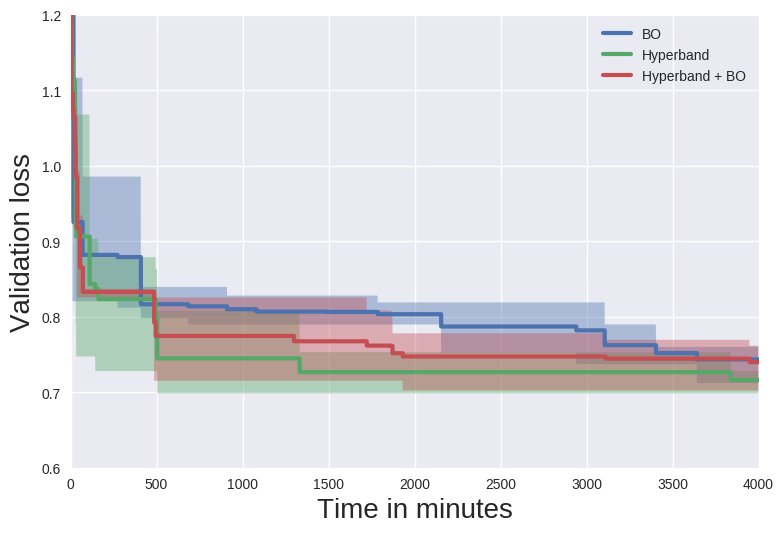
\includegraphics[width=7.2cm]{img_hyperopt/cifar_10_aggregate_best_val_loss_per_minute}}
	\end{minipage}
	\begin{minipage}[b]{.49\linewidth}
		\centering
		\centerline{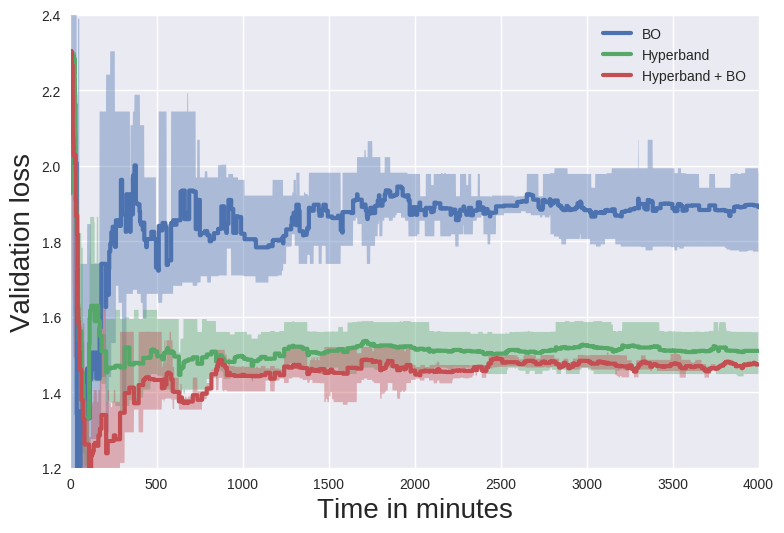
\includegraphics[width=7.2cm]{img_hyperopt/cifar_10_aggregate_median_val_loss_per_minute}}
	\end{minipage}
	\caption{(Left) Loss of the best model found at a given time by each method. (Right) Running median of the loss of all tested models for each method.}
	\label{fig:combining_loss}
\end{figure}

The metric that matters when comparing methods is the loss of the best model found at a given time, and is illustrated in Fig.~\ref{fig:combining_loss} for the two individual methods and their combination (5 run each). 
These results suggest that Bayesian optimization performs slightly worse than both other methods, and that Hyperband with Bayesian optimization finds a better model quicker than Hyperband. However, due to the stochastic nature of the methods, many more runs would be needed to draw definite conclusions from this metric. 

It might be more informative to look at the running median of the loss of all models trained at a given time. Even if in the end only the best model matters, the running median gives us an idea of the quality of the models tried. Bayesian optimization performs notably worse than the other two methods. Hyperband and Hyperband + BO have similar performance, though Hyperband + BO seems slightly better.

%%%%%%%%%%%%%%%%%%%%%%%%%%%%%%%%%%
\subsection{Discussion}

Due to the part of chance in all three methods, five runs are not enough to draw definite conclusions on their performance. Ideally hundreds of runs would have been needed, and the computational cost of this endeavor was the main reason we did not pursue further this problem.

While the seemingly low performance improvement of combining Hyperband and Bayesian optimization may be discouraging, there were two problems with our specific approach. 

As mentioned previously, since Bayesian optimization is usually sequential, we normalized the results of the acquisition function to make it a probability distribution from which the models to train were sampled. This was a terrible idea, as the resulting distribution was extremely close from a uniform distribution. This is because the expected improvement outputs values in a small range, i.e. the difference between the maximum and the minimum is at most a few orders of magnitude. When normalized, those extreme values would not be particularly likely, even with just a small hyper-parameters space of $19 200$ combinations. In effect, this is why our version of Hyperband + BO performed barely better than Hyperband alone. 

One potential solution would have been to use the "liar" strategy. After choosing a model but before training it, it is added to the training set with a low performance and the acquisition function is re-computed. The "lie" of the low performance has for effect of discouraging the acquisition function from giving high values to the surrounding models, and the argmax will be a completely different model. Repeating this process allow drawing many models simultaneously. 

When drawing a large group of models at the same time like Hyperband requires, the cost of this process becomes important as the Gram matrix of the Gaussian process needs to be inverted many times. The incremental Cholesky decomposition presented in Section~\ref{sec:cholesky} could be used to make the process faster.

Informal observations of the chosen models revealed a second problem. After a few iterations, many of the models chosen tended to be fully trained by the time of Hyperband's first evaluation (after 3 minutes of training) and start overfitting immediately after. This was due to how Bayesian optimization handled the training time. Since all models were trained at least 3 minutes, but only some trained longer, the Gaussian process predictions were much more accurate at 3 minutes than at 27 minutes. This was our reason to use the prediction at 3 minutes, though with side effect described.

While using the prediction at 27 minutes instead would avoid the overfitting, it would also discard a lot of information as the predictions of all the models trained only partially would have reverted to the prior of the covariance function by 27 minutes. It would be better to design a special kernel to deal with only this hyper-parameter and that does not revert quickly. Inspiration for this kernel could be found in~\textcite{domhan2015} as they study models to extrapolate learning curves.

%%%%%%%%%%%%%%%%%%%%%%%%%%%%%%%%%%%%%%%%%%%%%%%%%%%%%%%%%%%%%%%%%%%%%%%%%%%%%%%%%%%%%%%%%%%%%%%
\section{Application: Classification of MRI Field-of-View}
\label{sec:isbi}

This section describes and extends work presented at ISBI 2017 (\textcite{bertrand2017ISBI}).

%%%%%%%%%%%%%%%%%%%%%%%%%%%%%%%%%%
\subsection{Dataset and problem description}

\begin{figure}[htb]
        \begin{subfigure}[b]{0.25\textwidth}
                \centering
                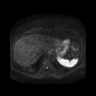
\includegraphics[width=.95\linewidth]{img_hyperopt/Abdomen_785}
        \end{subfigure}%
        \begin{subfigure}[b]{0.25\textwidth}
                \centering
                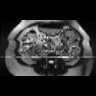
\includegraphics[width=.95\linewidth]{img_hyperopt/Abdomen_1050}
        \end{subfigure}%
        \begin{subfigure}[b]{0.25\textwidth}
                \centering
                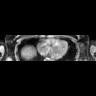
\includegraphics[width=.95\linewidth]{img_hyperopt/Abdomen_5115}
        \end{subfigure}%
        \begin{subfigure}[b]{0.25\textwidth}
                \centering
                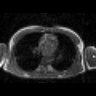
\includegraphics[width=.95\linewidth]{img_hyperopt/Chest_6810}
        \end{subfigure}
        
        \vspace*{2mm}
        
        \begin{subfigure}[b]{0.25\textwidth}
                \centering
                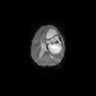
\includegraphics[width=.95\linewidth]{img_hyperopt/Head_13330}
        \end{subfigure}%
        \begin{subfigure}[b]{0.25\textwidth}
                \centering
                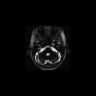
\includegraphics[width=.95\linewidth]{img_hyperopt/Head_14031}
        \end{subfigure}%
        \begin{subfigure}[b]{0.25\textwidth}
                \centering
                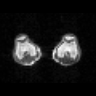
\includegraphics[width=.95\linewidth]{img_hyperopt/Legs_13170}
        \end{subfigure}%
        \begin{subfigure}[b]{0.25\textwidth}
                \centering
                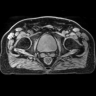
\includegraphics[width=.95\linewidth]{img_hyperopt/Pelvis_23016}
        \end{subfigure}
        \caption{Images from the MR dataset showing the variety of classes and protocols.}
        \label{fig:dataset}
\end{figure}

Given an MRI volume we would like to know which anatomical regions are contained in it and their position in the volume. Since MRI data are acquired in a slice by slice approach, we reduce the problem to a two dimensional classification task of axial slices (into head, chest, abdomen, pelvis, legs and spine).

\begin{table}[htb]
	\centering
	\begin{tabular}{ | l | c | r | }
		\hline
		Body Part & \# Volumes & \# Slices \\ \hline
		Head & 404 & 17011 \\
		Chest & 186 & 6897 \\
		Abdomen & 367 & 15486 \\
		Pelvis & 351 & 17962 \\
		Legs & 99 & 12868 \\
		Spine & 390 & 9790 \\
		\hline
	\end{tabular}
	\caption{Content of the dataset.}
	\label{table:dataset}
\end{table}

The dataset consists of MRI images coming from a variety of hospitals and machines across the world (such as the \textit{Centre Hospitalier Lyon-Sud, France} or \textit{ Johns Hopkins University, USA}). As a consequence the images are highly varied in terms of protocols (see Figure~\ref{fig:dataset}) as well as resolution, number of volumes per class and number of slices per volume. Table~\ref{table:dataset} sums up the content of our dataset.

The dataset is splitted into a training set for the optimization of the weights of the networks, a validation set for model selection (optimization of the hyper-parameters) and a test set for model evaluation (respectively $50 \%$, $25 \%$, $25 \%$ of the database). The separation is done volume-wise to take into account intra-subject slices correlations. Volumes containing multiple classes are split by anatomical regions and can end up in different sets. This raises the difficulty of the task since, in case of overfitting, predictions will be wrong at validation or testing phases.

%We also stratified classes across sets, giving us a proportion of slices per class close to the proportion of volumes per class.

Finally, each slice is subject to a unique step of preprocessing: it is resized to $128 \times 128$ pixels, a good trade-off between time constraints and quality of information.

Data augmentation is used and consists in generating 80 000 images per epoch. The augmentation is done by applying translations, shearing and rotations, zooming, and adding Gaussian noise.

%%%%%%%%%%%%%%%%%%%%%%%%%%%%%%%%%%
\subsection{Baseline results}

\begin{figure}[htb]
	\centering
	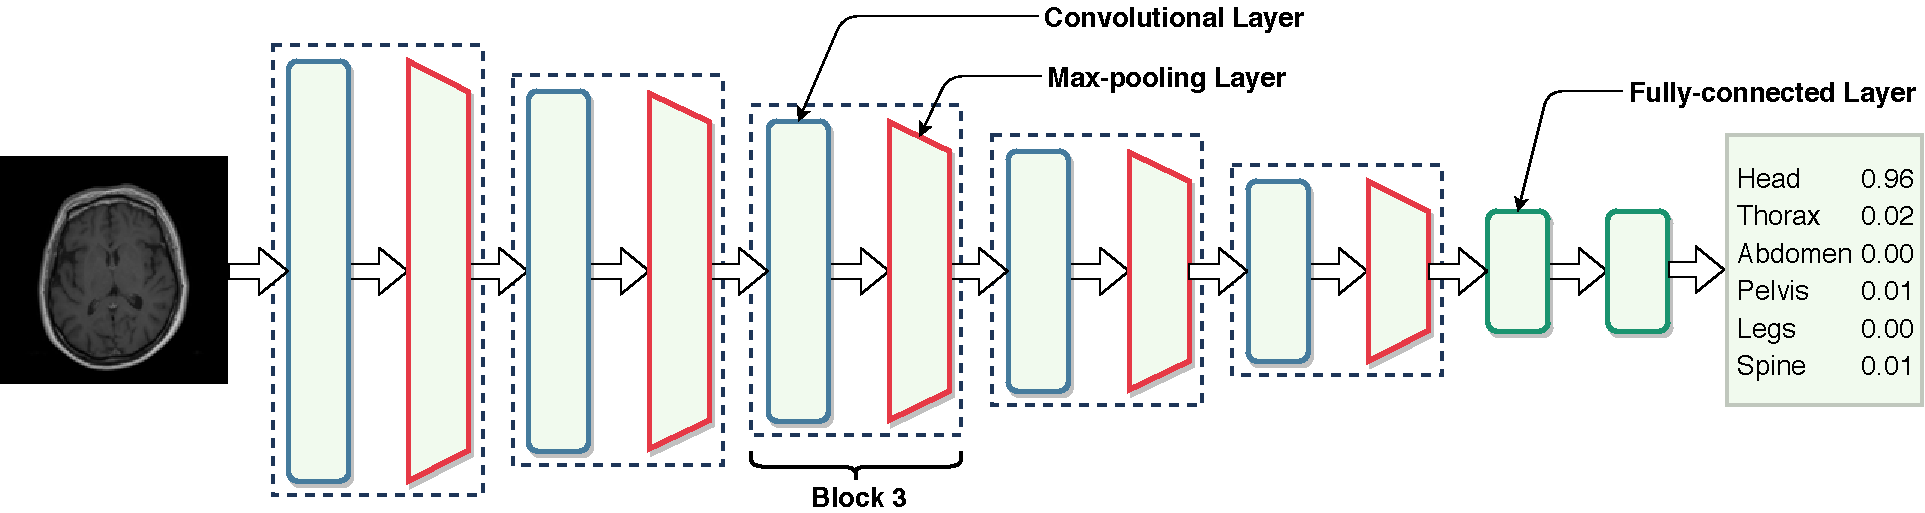
\includegraphics[width=\linewidth]{img_hyperopt/baseline.pdf}
	\caption{Baseline network used to solve the problem.}
	\label{fig:baseline}
\end{figure}

Starting from a standard VGG architecture (\textcite{simonyan2014}), we modified it manually until settling on the following model, shown in Figure~\ref{fig:baseline}: it is divided into 5 blocks, each comprising a convolution layer of 64 filters of size $3\times 3$, followed by a rectified linear unit (ReLu) and a max-pooling layer. The network ends with 2 fully-connected layers (respectively 4096 and 1024 units) interleaved with ReLU activations and terminated with a softmax decision layer. This network was trained by minimizing the categorical cross-entropy loss weighted by class frequency, using stochastic gradient descent (SGD) with a learning rate of $10^{-3}$, Nesterov momentum ($m = 0.9$) and decay ($d = 10^{-6}$) for 30 epochs.

\begin{table}
    \centering
    \newcommand\items{6}   %Number of classes
    \arrayrulecolor{white} %Table line colors
    \noindent\begin{tabular}{cc*{\items}{|E}|}
    \multicolumn{1}{c}{} &\multicolumn{1}{c}{} &\multicolumn{\items}{c}{\textbf{Predicted}} \\ \hhline{~*\items{|-}|}
    \multicolumn{1}{c}{} & 
    \multicolumn{1}{c}{} & 
    \multicolumn{1}{c}{\rot{Head}} & 
    \multicolumn{1}{c}{\rot{Chest}} & 
    \multicolumn{1}{c}{\rot{Abdomen}} &
    \multicolumn{1}{c}{\rot{Pelvis}} & 
    \multicolumn{1}{c}{\rot{Legs}} & 
    \multicolumn{1}{c}{\rot{Spine}} \\ \hhline{~*\items{|-}|}
    \multirow{\items}{*}{\rotatebox{90}{\textbf{Actual}}} 
    &Head  & 96 & 0 & 1 & 2 & 1 & 0   \\ \hhline{~*\items{|-}|}
    &Chest  & 1 & 57 & 13 & 28 & 1 & 0   \\ \hhline{~*\items{|-}|}
    &Abdomen  & 0 & 1 & 88 & 10 & 0 & 1   \\ \hhline{~*\items{|-}|}
    &Pelvis  & 1 & 0 & 9 & 81 & 8 & 1   \\ \hhline{~*\items{|-}|}
    &Legs  & 0 & 0 & 0 & 19 & 81 & 0   \\ \hhline{~*\items{|-}|}
    &Spine  & 0 & 1 & 3 & 2 & 0 & 94   \\ \hhline{~*\items{|-}|}
    \end{tabular}
    \caption{Confusion matrix for the baseline on the test set, in percent.}
	\label{table:conf_matrix_baseline}
\end{table}

We achieve a $14 \%$ error rate with most of the error focused on the chest. Examining the confusion matrix (Table~\ref{table:conf_matrix_baseline}), we note that the abdomen, pelvis and legs images have most of their errors located with anatomically adjacent regions. Further examinations of the misclassified images revealed they were for the most part located at the boundaries of their classes. These errors make sense as these boundaries are ill-defined and varies from one volume to the next. 

%%%%%%%%%%%%%%%%%%%%%%%%%%%%%%%%%%
\subsection{Hyper-parameter optimization}

\begin{figure}[htb]
	\centering
	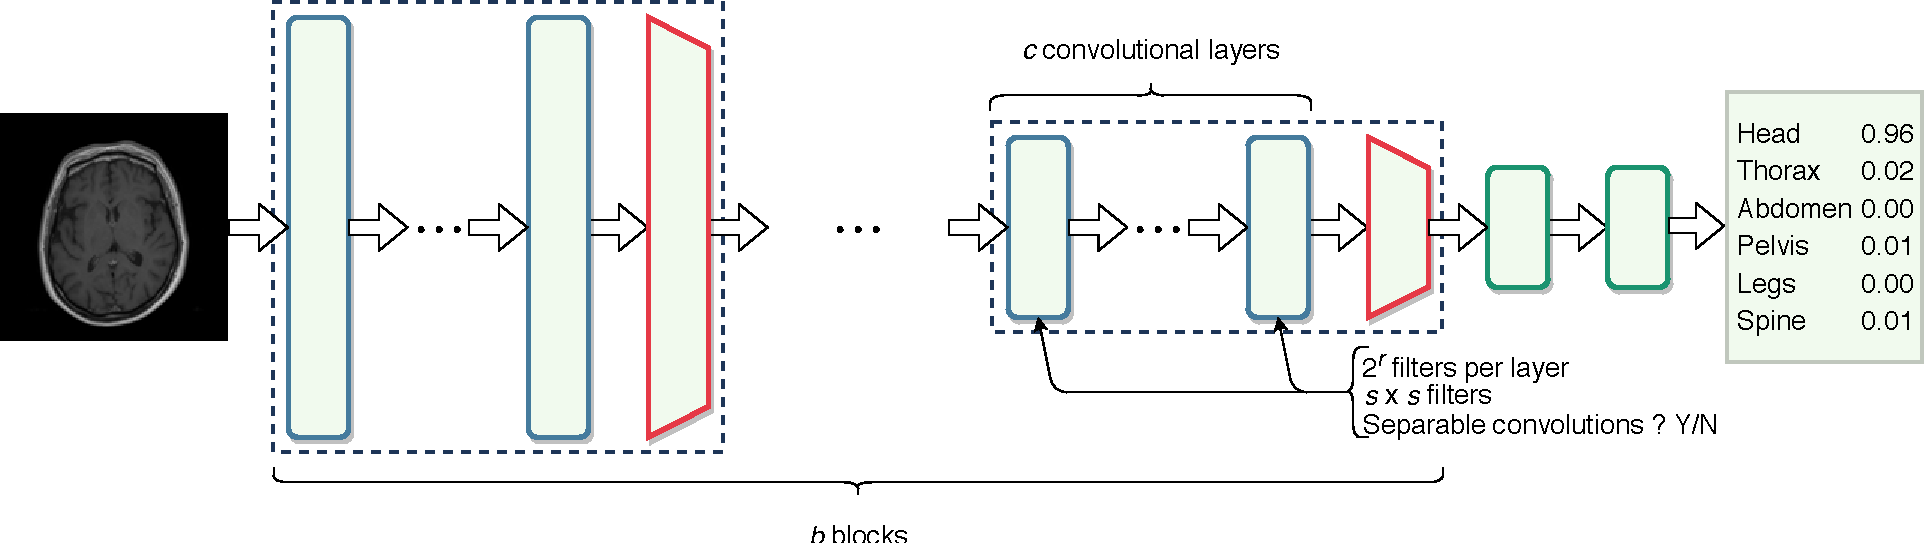
\includegraphics[width=\linewidth]{img_hyperopt/hyperspace.pdf}
	\caption{Variations on the baseline allowed in our search.}
	\label{fig:hyperspace}
\end{figure}

By relaxing some structural parts of our baseline architecture we define a large family of models. This hyper-parametric family has the following structure (see Figure~\ref{fig:hyperspace}): (1) $b$ convolution blocks, each including $c$ convolutional layers of $2^r$ filters of size $s \times s$ interleaved with ReLU activations and terminated by a max-pooling layer, (2) the fully-connected layers as in our baseline architecture, and (3) a final softmax decision layer. 

The last hyper-parameter is whether the convolutions are separable or not. Separable convolutions are two different convolutional layers using $1 \times 3$ filters then $3 \times 1$. This leads to a $33 \%$ reduction in the number of weights often without negative impact on the model performance.

Changes within this parametric space of models may drastically transform the optimization landscape, requiring to adjust the training setting accordingly (in our case: learning rate and batch size, all other settings remaining identical). 
These architecture hyper-parameters and training settings form the hyper-parameter space. The ranges of those hyper-parameters, detailed in Table~\ref{table:hyper}, were defined so as to fulfill memory (less than 12GB) and time constraints (training should last less than one day).

While many more hyper-parameters could have been considered, the ones we chose already define a search space of 34 300 models, well-above our capacity to fully explore. Those hyper-parameters were chosen as they were considered to have the highest impact on the performance by a mix of intuition and experience. A more systematic approach would likely yield better results, though at a greater computational cost.

\begin{table}
	\centering
	\arrayrulecolor{black}
	\begin{tabular}{ | l | c | r | }
		\hline
		Name & Range & Baseline \\ \hline
		Number of blocks & $b \in [1 ; 5]$ & $5$ \\
		Number of convolutional layers per block & $c \in [1 ; 5]$ & $1$ \\
		Number of filters per convolutional layer & $2^{r}, r \in [2, 8]$ & $64$ \\
		Size of the filters & $ s \in \{3 ; 5\}$ & $3$ \\
		Separable Convolutions & $e \in \{\text{Yes}, \text{No}\}$ & No \\
		Learning Rate & $10^{l}, l \in [-7 ; 0]$ & $0.001$ \\
		Batch Size & $2^{a}, a \in [2 ; 8]$ & 8 \\
		\hline
	\end{tabular}
	\caption{Description of the hyper-parameters, with their range and and the baseline value.}
	\label{table:hyper}
\end{table}

To explore this hyper-parameter space, we used Bayesian optimization, as described in Section~\ref{sec:bo}. We chose the Expected Improvement as our acquisition function, and we used the loss on the validation set as the value the Gaussian process must predict. Every network was trained for 30 epochs, and we trained a total of 300 models. The first model picked by the Bayesian optimization is usually chosen randomly, here it made sense to start from the baseline as it was already trained.

\begin{figure}[htb]
	\centering
	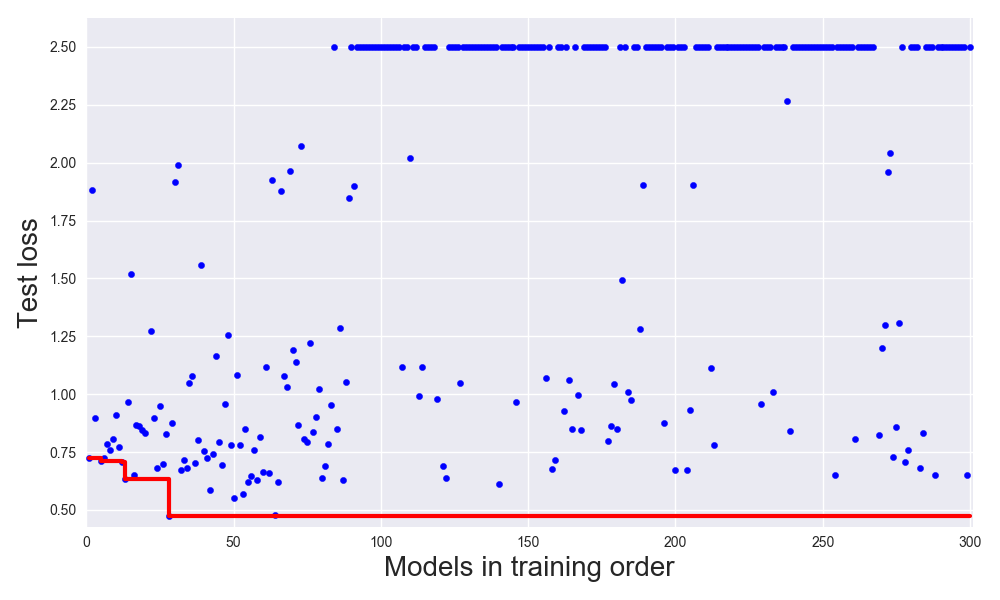
\includegraphics[width=\linewidth]{img_hyperopt/mrfov_bo_ei}
	\caption{Performance of the models in the order they were trained. Each dot is a model. The red line represents the performance of the best model found until this point. The models with a loss of $2.5$ are models that couldn't be trained as they were too big.}
	\label{fig:mrfov_bo_ei}
\end{figure}

At the end, our optimization process yields a collection of models ranked by their performance. The quality of this assessment is naturally limited since the size of the validation set used in this respect cannot encompass the diversity of clinical reality. Cross-validation could be used to get a better estimator of the performance, but we cannot practically afford its costs. 

Figure~\ref{fig:mrfov_bo_ei} shows the performance of the models in the order they were trained. The baseline is quickly improved upon and the best model is found after 33 iterations. Another model with similar performance is found after 55 iterations. Starting at iteration 90, most of the chosen models are too big to fit in memory and therefore unable to train. While the fact that no previously chosen models were too memory intensive but suddenly most chosen models are may seem surprising, this can be explained for two reasons.

The first model of the process was our hand-crafted baseline, which had good performance. This likely allowed a good initialization of the Gaussian process, and the following models explored the area around the baseline. As models explored further and further than the baseline, eventually one was chosen that was too big to fit in memory. This argument is speculation that should be confirmed by repeating the Bayesian optimization many times with a different initialization every time. Lack of resources prevented us from exploring this point further.

The second argument explains why most models became impossible to train as soon as the first of those was chosen. This is due to how we handled models impossible to train for memory limitations. We chose to simply remove such models from the search space. However the acquisition function still gives a high priority to this region of space and a surrounding model is chosen that is also likely to be too big. Since we remove those models on subsequent iterations, the acquisition function never learns to not go there.

An alternative way to handle un-trainable models would have been to choose an arbitrarily high loss for those models. This violate the smoothness assumption of the Gaussian process and would have affected strongly the prediction on nearby models, discouraging the acquisition function from choosing them. This would have also disqualified nearby models that fit in memory, which was our reason for not doing that in the first place. 

It is not clear which strategy is better. Choosing a high loss sacrifices some valid models, but saves time by testing less un-trainable models. On the other hand, an un-trainable model fail immediately at model creation, so the gain in time is minor. 
But independently of the chosen strategy, the fact that some combinations lead to model too big to fit in memory highlights a flaw in the design of the hyper-parameters space and the resulting networks architectures. The un-trainable models are models with a low number of blocks but a high number of filters per layer. With one block and 64 filters per layer, the feature maps of the last convolutional layer are of size $64 \times 48 \times 48$, meaning the following fully-connected layer have $64 \times 48 \times 48 \times 4096 = 603,979,776$ weights. Since each block ends with a max-pooling layer, the number of weights quickly become manageable with additional blocks. 

\begin{table}
    \centering
    \newcommand\items{6}   %Number of classes
    \arrayrulecolor{white} %Table line colors
    \noindent\begin{tabular}{cc*{\items}{|E}|}
    \multicolumn{1}{c}{} &\multicolumn{1}{c}{} &\multicolumn{\items}{c}{\textbf{Predicted}} \\ \hhline{~*\items{|-}|}
    \multicolumn{1}{c}{} & 
    \multicolumn{1}{c}{} & 
    \multicolumn{1}{c}{\rot{Head}} & 
    \multicolumn{1}{c}{\rot{Chest}} & 
    \multicolumn{1}{c}{\rot{Abdomen}} &
    \multicolumn{1}{c}{\rot{Pelvis}} & 
    \multicolumn{1}{c}{\rot{Legs}} & 
    \multicolumn{1}{c}{\rot{Spine}} \\ \hhline{~*\items{|-}|}
    \multirow{\items}{*}{\rotatebox{90}{\textbf{Actual}}} 
    &Head  & 94 & 0 & 1 & 1 & 2 & 0   \\ \hhline{~*\items{|-}|}
    &Chest  & 0 & 93 & 5 & 1 & 1 & 0   \\ \hhline{~*\items{|-}|}
    &Abdomen  & 0 & 2 & 85 & 10 & 2 & 1   \\ \hhline{~*\items{|-}|}
    &Pelvis  & 1 & 2 & 4 & 86 & 6 & 1   \\ \hhline{~*\items{|-}|}
    &Legs  & 0 & 4 & 1 & 19 & 76 & 0   \\ \hhline{~*\items{|-}|}
    &Spine  & 0 & 1 & 1 & 0 & 2 & 96   \\ \hhline{~*\items{|-}|}
    \end{tabular}
    \caption{Confusion matrix for the best model on the test set, in percent.}
	\label{table:conf_matrix_best}
\end{table}

The best model found with Bayesian optimization has an error rate of $10 \%$, an improvement of $4 \%$ over the baseline. Looking at the confusion matrix in Table~\ref{table:conf_matrix_best}, there is a significant improvement in the classification of chest, going from $57 \%$ accuracy in the baseline to $93 \%$ accuracy. The other classes have similar accuracy as the baseline. Most of the errors are abdomen and legs slices located at the boundaries of the pelvis.

Looking at the architectures of the two best models that have very similar error rates, the first one only deviates from the baseline by having two convolutional layers per block but only $32$ filters per convolutional layer and a higher batch size of $32$. The second model however is completely different. It has only 4 blocks with 3 convolutional layers per block, uses separable convolutions, with a smaller batch size of 4 and learning rate of $10^{-4}$.

The last important factor to consider is the total number of weights. The baseline model had $6,713,226$ weights, the best model had $5,468,778$, a $19 \%$ reduction. The second best model had $13,927,114$ weights due to using one less block than the other two models. Once again most of the weights are caused by the transition from the last convolutional layer to the first fully-connected layer. To improve on those results the first step would be to better design this transition, either by controlling the number of max-pooling layers or by replacing the fully-connected layers with convolutional layers, as is typical of modern convolutional neural networks. 

\subsection{From probabilities to a decision}

\begin{figure}[htbp]
	\centering
	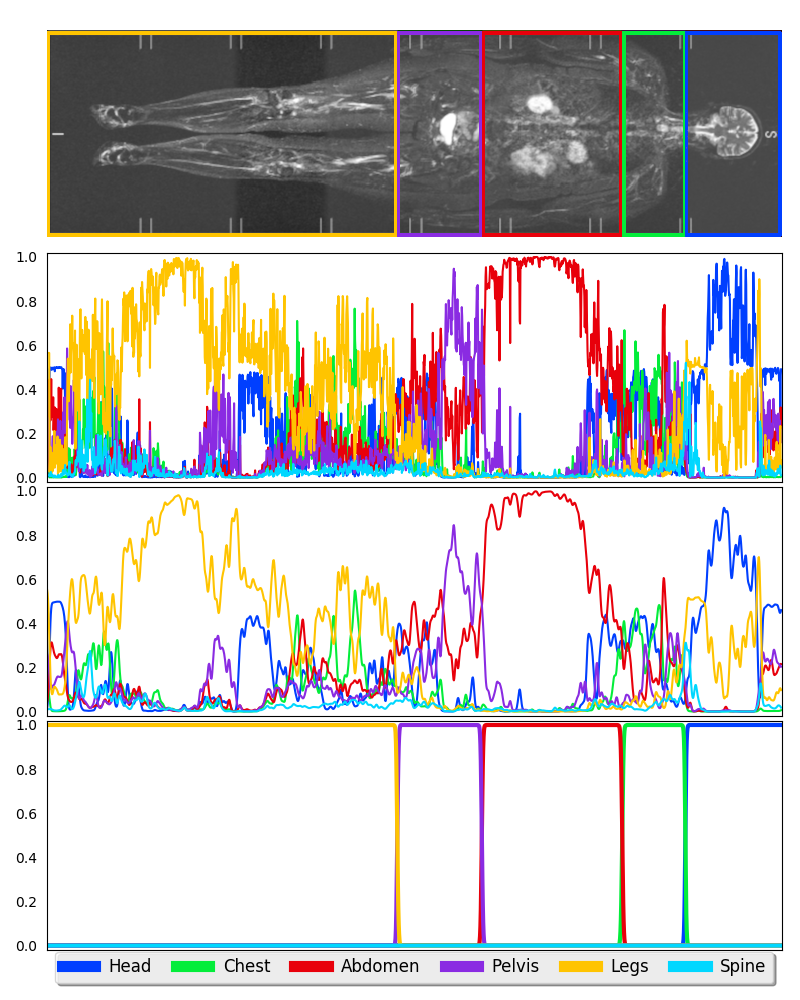
\includegraphics[width=\linewidth]{img_hyperopt/fullbody}
	\caption{Slice by slice prediction on a full body volume. From top to bottom: (a) Image and ground truth. (b) Raw model prediction. (c) After smoothing. (d) After selecting the best transitions.}
	\label{fig:full_body}
\end{figure}

Even though we made the choice of processing the data at the slice level, the slices form volumes and we are interested in a decision at the volume level. The first question is: does the model classifies two successive slices similarly ? This is expected since successive slices are anatomically close and have a similar structure. If the model gives very different predictions, this could be a sign that it relies on noise patterns instead of the anatomical structures.

To answer this question, we processed a full body volume by classifying each of its slices through our best model. 
%For each slice, the predicted class is the one with a probability higher than $0.7$, and if no class meets this criterion, then we do not choose any. 
As we can see in Figure~\ref{fig:full_body}, the network is able to identify all body parts, despite the slices being processed independently. Nevertheless the network tends to misclassify the boundaries between regions, notably legs/pelvis and pelvis/abdomen. It also mistakenly identifies the empty slices above the head as being pelvis with a high confidence. This might be indicative of overfitting as those slices contain only noise. Interestingly, the straps used to hold the patient down, visible as the bands with high intensity on the extremities and low intensities on the body, trigger the network every time into the pelvis class. This is likely due to the rarity of those straps in the dataset.

But we are not interested in the mere probabilities, we want to take an actual decision. Therefore we need a decision scheme. A very simple one would be a threshold, say $0.7$, over which we consider the slice to be part of the class. However the predictions from the network are too noisy (see Figure~\ref{fig:full_body}-b), and this approach gives regions broken in multiple parts with messy boundaries.

A first step is to smooth the probabilities curves with a Gaussian filter, as illustrated in Figure~\ref{fig:full_body}-c. This makes the predictions easier to read, and we can see that on this example the predictions are correct almost everywhere except for the chest. Additionally, the pelvis is preceded and followed by the abdomen, which is of course impossible.

From this last observation, we note that our goal is to find contiguous anatomical regions, delimited by a starting slice $Z^m_i$ and an ending slice $Z^M_i$, where $i$ is the index of the region in anatomical order (legs - pelvis - abdomen - chest - head) and $Z$ is the slice number. Those boundaries must be such that $\forall i \in [1; N], Z^m_i < Z^M_i$. The network outputs the probability of a slice to belong to a region $P_i \left( Z \right)$.

The optimal boundary slices are the solutions to the following linear program:
\begin{equation}
    \begin{array}{ll@{}ll}
    \text{minimize}  & - \displaystyle\sum\limits_{i=1}^{N} \int_{Z_i^m}^{Z_i^M} P_i(z) dz &\\
    \text{subject to}&  Z^m_{i+1} \ge Z^M_i,  &i=1 ,..., N
    \end{array}
    \label{eq:optimal_boundary}
\end{equation}
The constraints specify that a region cannot start earlier than the end of the previous region.

The Lagrangian is:
\begin{equation}
    \mathcal{L} \left( Z_i^m, Z_i^M, \lambda \right) = - \displaystyle\sum\limits_{i=1}^{N} \int_{Z_i^m}^{Z_i^M} P_i(z) dz
                                                        - \displaystyle\sum\limits_{i=1}^{N} \lambda_i \left( Z^m_{i+1} - Z_i^M \right)
\end{equation}
From the partial derivatives, we obtain:
\begin{align*}
    \frac{\partial \mathcal{L}}{\partial Z_i^m} &= P_i \left( Z_i^m \right) - \lambda_{i-1} \\
    \frac{\partial \mathcal{L}}{\partial Z_i^M} &= - P_i \left( Z_i^M \right) + \lambda_{i}
\end{align*}
Setting the derivatives at zero, the optimal boundary slices must verify:
\begin{equation}
    P_i \left( Z_i^M \right) = P_{i+1} \left( Z_{i+1}^m \right)
\end{equation}
This last constraint means that the boundary slices must be at the intersections between two successive regions. To clarify, a slice where the probability of belonging to the pelvis is equal to the probability of belonging to the abdomen is a potential boundary slice, but an intersection slice between pelvis and head is not.

To find the optimal boundary slices, we find all the valid intersection slices, construct all the valid sets of transitions and compute the function defined in Equation~\ref{eq:optimal_boundary}. The minimum is the optimal set of boundary slices. An example is shown in Figure~\ref{fig:full_body}-d.

This scheme is robust because of its properties: each region is at most one contiguous block (they can also be not present), the regions are always in anatomical order and it allows for many misclassified slices. 

\subsection{Conclusion}

We have shown how to use Bayesian optimization to the concrete problem of MR FOV classification. The gain in performance between our handcrafted model and the best model clearly shows the value of automating the search of hyper-parameters, even with a limited budget.

The search was vulnerable to all the weaknesses of Bayesian optimization: the process was sequential (only one model trained at a time), we were limited in the hyper-parameters we could use (no conditional hyper-parameters) and the kernel was stationary. 
%As presented in Section~\ref{ssec:nosta}, work has been done on all those limitations and should be incorporated to improve the process. Other search methods could also be used, such as Hyperband (Section~\ref{sec:cap}). 

Another problem encountered is how to deal with models that cannot be trained (because they require too much memory for example). Not putting them in the training set will just let the search pick other similar models, but putting an arbitrarily high value is not ideal either as the Gaussian process will smoothly interpolate to that value, even though there is a discontinuity in that region (between the models that can and cannot be trained).

Regarding the final models, testing at the volume level has shown that the models are robust and can generalize. Still, the neural network was not enough to obtain smooth coherent predictions, and we presented a decision scheme to fix that.

Further work on this problem would involve improving the dataset by adding new volumes, new anatomical regions and defining stricter boundaries between regions. The model could also be improved by using a cyclic learning rate, spatial dropout on the convolutional layers and replacing the fully-connected layers with convolutional layers. More care should be put in designing the hyper-parameter space, to limit the number of un-trainable models.

%%%%%%%%%%%%%%%%%%%%%%%%%%%%%%%%%%%%%%%%%%%%%%%%%%%%%%%%%%%%%%%%%%%%%%%%%%%%%%%%%%%%%%%%%%%%%%%
% \section{Conclusion}

% When to optimize and with which method ?


%%%%%%%%%%%%%%%%%%%%%%%%%%%%%%%%%%%%%%%%%%%%%%%%%%%%%%%%%%%%%%%%%%%%%%%%%%%%%%%%%%%%%%%%%%%%%%%
%                                     TRANSFER LEARNING                                       %
%%%%%%%%%%%%%%%%%%%%%%%%%%%%%%%%%%%%%%%%%%%%%%%%%%%%%%%%%%%%%%%%%%%%%%%%%%%%%%%%%%%%%%%%%%%%%%%
\chapter{Transfer Learning}
\label{chap:transfer}

\begin{chapabstract}
 Coucou
\end{chapabstract}

\minitoc

\newpage

%%%%%%%%%%%%%%%%%%%%%%%%%%%%%%%%%%%%%%%%%%%%%%%%%%%%%%%%%%%%%%%%%%%%%%%%%%%%%%%%%%%%%%%%%%%%%%%
\section{The many different faces of transfer learning}

Despite all the modern successes of deep learning, the set of tasks that it can solve and that are also related to medical imaging is quite small. A frequent situation that arises is then, if a network is able to segment a particular organ in a particular imaging protocol, is it possible to train a network to segment the same organ in another imaging protocol? Or train a network for a particular population from a network trained for a different population? It is expected that, since the task stays identical, it should be possible to leverage the knowledge from the first database to increase the performance on the second database. This is one of the problem addressed by transfer learning.

There are various reasons why transfer learning may be useful. In the medical field in particular, the acquisition of data is costly and time-consuming, and labeling or segmenting the acquired data to build a training database even more so. It is very common to have only a handful of patients from a particular population. Therefore, using every available bit of data is necessary, and re-using them would be even better. Additionally, modern deep learning models tend to be costly to train, in both resources and time. It is also common to wish to extend a working deep learning model to a new slightly different use-case. It would then be more efficient to re-use the model instead of starting from scratch. All these reasons justify the need for transfer learning.

\begin{figure}[h]
    \centering
	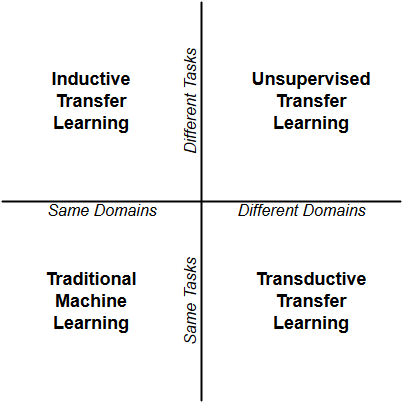
\includegraphics[width=0.5\textwidth]{img_transfer/transfer_types.png}
    \caption{Transfer learning can be divided into four categories depending on how the domains and the tasks are related.}
    \label{fig:transfer_types}
\end{figure}

Following the notation of~\textcite{pan2010TNDE}, we define the \textit{domain} as a feature space $\mathcal{X}$ and a probability distribution $P\left( \mathrm{X} \right)$. A \textit{task} is composed of a label space $\mathcal{Y}$ and an objective predictive function $f$ which is learned from the training data (i.e. pairs of $\{ x_i, y_i \}$ where $x_i \in \mathcal{X}$ and $y_i \in \mathcal{Y}$). The transfer is done from a \textit{source} domain and task to a \textit{target} domain and task. These notions forms the two axes according to which transfer learning methods are divided. How are the source and target domains related, and how are the source and target tasks related? These axes result in four different problems as shown in Figure~\ref{fig:transfer_types}. 

Inductive transfer learning is the category of problems where the source and target domains are identical, while the source and target tasks are different, but related. An example of such a problem would be an image database where the source task is to detect the presence or absence of particular objects and the target task is to locate those objects in the image. Transductive transfer learning is the category where the source and target domains are different but related, while the source and target tasks are identical. An example that we study in Section~\ref{sec:kidney_seg} is the segmentation of the kidney in 3D ultrasound images, where the source domain is healthy adults and the target domain is sick children. Unsupervised transfer learning happens when both the domains and the tasks are different. In this setting, labels are unavailable for both source and target. In all three cases, transfer of knowledge is possible by exploiting the nature of the differences between the domains and the tasks.

In this section we briefly present these three kinds of transfer learning. Then Section~\ref{ssec:deep_transfer} focuses on transfer learning in the context of deep learning.

If both the domains and the tasks are identical, this is simply standard machine learning and not transfer learning.

%%%%%%%%%%%%%%%%%%%
\subsection{Inductive Transfer Learning}
\label{ssec:inductive}

In this setting, the source and target tasks are different, while the source and target domains stay the same. 

%%%%%%%%%%%%%%%%%%%
\subsection{Transductive Transfer Learning}
\label{ssec:transductive}

%%%%%%%%%%%%%%%%%%%
\subsection{Unsupervised Transfer Learning}
\label{ssec:unsupervised}

There has been relatively little work in this setting.~\textcite{dai2008ICML} propose a \textit{self-taught clustering} algorithm which aim to cluster a small unlabeled target dataset at the same time as a big unlabeled source dataset. By learning a common feature space, clustering on the target dataset is improved.

\textcite{chang2018} developed a method to learn a bank of multi-scale convolutional filters from a large unlabeled source dataset and a small target dataset, which can then used in a convolutional neural network to solve classification tasks. Only the construction of the filters bank is done without labels. Application on various biomedical applications shows a clear improvement in performance over using only the target dataset.

%%%%%%%%%%%%%%%%%%%
\subsection{Transfer Learning and Deep Learning}
\label{ssec:deep_transfer}

One method has become the \textit{de facto} face of transfer learning for deep neural networks, due to its simplicity and versatility: fine-tuning (\textcite{hinton2006},~\textcite{bengio2007NIPS}). The idea is that the features learned by a neural network are generic enough, so that it becomes interesting to re-use them on a different domain, for a different task, or both. No modifications to the architecture are done. The only difference is that the weights of the network are not initialized randomly, but set to the final weights learned on the source domain.

It is not always necessary, or even a good idea, to re-train the whole network. If the target dataset is too small, full fine-tuning risks overfitting. But then, which layers should be fine-tuned? Lower layers tend to be more generic, while higher layers tend to be specialized to the task (\textcite{yosinski2014NIPS}), suggesting that it would be better to fine-tune only the last $n$ layers of the network. An additional advantage is that it is faster as there is no need to back-propagate to the lower layers. The exact value of $n$ is entirely problem-specific, the closer the domains and the tasks are, the less layers need to be fine-tuned.

Moreover the source dataset does not need to be closely related to the target dataset. A network trained for classification on the ImageNet dataset (\textcite{imagenet}) can be fine-tuned on other natural images dataset for classification or even detection and improve the results over training from scratch (\textcite{oquab2014CVPR},~\textcite{razavian2014CVPR}).

An alternative to fine-tuning is feature extraction (\textcite{donahue14PMLR}). It is similar to fine-tuning in that it uses the fact that the features learned by the lower layers of a neural network are fairly generic. But instead of modifying the higher layers of the network, here they are discarded and the output of the lower layers are used as features for a completely different model, not necessarily a neural network. Features extracted from natural images have been shown to be useful to medical images (\textcite{shin2016},~\textcite{bar2015ISBI},~\textcite{vanginneken2015ISBI}).

So far we have assumed the model is trained first on a task, then later adjusted for another. But if we know from the start the multiple tasks, we might as well train on them at the same time. This is the idea of multitask training (\textcite{caruana1995NIPS},~\textcite{caruana1997},~\textcite{collobert2008ICML}). It consistently gives better results on both tasks than sequential transfer methods and should be used if possible.

Autoencoders (\textcite{ballard1987},~\textcite{bengio2007NIPS}) are neural networks learned in an unsupervised manner. The goal of the network is to reconstruct its input from a compressed representation of the data that it will learn. The first part of the network progressively compresses the input while the second part decompresses it. That first part can then be used as a pre-trained network for other datasets and tasks (\textcite{bengio2007NIPS},~\textcite{vincent2008ICML},~\textcite{erhan2010JMLR}). The representation learned by the autoencoder can also be used as the features of another model, which is helpful even for distant domains such as natural images and MR images (\textcite{gupta2013ICML}). More generally, unsupervised pre-training on natural images has successfully been used to improve results on medical imaging tasks (\textcite{schlegl2014MICCAI},~\textcite{hofmanninger2015CVPR}).

%Finetuning across domains and tasks~\textcite{tzeng2015ICCV}.


%GAN DA~\textcite{kamnitsas2017IPMI}

%%%%%%%%%%%%%%%%%%%%%%%%%%%%%%%%%%%%%%%%%%%%%%%%%%%%%%%%%%%%%%%%%%%%%%%%%%%%%%%%%%%%%%%%%%%%%%%
\section{Transformation Layers}
\label{sec:transfo}

Here we propose to introduce ``transfer'' layers within the original model in order to adapt feature maps to the new dataset. We expect these layers to selectively adapt the network to children data while maintaining the network performance on adults.

%We selected six emplacements for adding layers: before the max-pooling and after the up-sampling, as shown in green in Figures ~\ref{fig:unet} and ~\ref{fig:block}. As each additional layer adds parameters and training time, but potentially allows for more capacity, we explored various combinations of emplacements to find the optimal trade-off. Each transfer block must have the same output size as its input to properly connect with the adjacent layer.

%As there is no obvious shape for the transfer layers, we designed a number of variations with different properties. The simplest was a single convolutional layer of $1 \times 1 \times 1$ filters. As $1 \times 1 \times 1$ convolutional layers do not capture locally spatial information, we also tested $3 \times 3 \times 3$ filters with the inconvenient of adding a high number of parameters (because we cannot reduce the number of filters). To solve this issue we used the following block: one $1 \times 1 \times 1$ convolutional layer with less filters to reduce dimensionality, followed by a max-pooling and a $3 \times 3 \times 3$ convolutional layer, then up-sampling and one last $1 \times 1 \times 1$ convolutional layer to recover the expected dimensionality. 
%One variant we tried was to make those layers residual. The intuition is that because the adults and the children are not so different, it might be easier to learn a correction of the feature maps rather than transform them directly.

When inserting new layers, it might be tempting to simply use standard convolutional layers. The problem is that as the parameters of these layers are fixed once the training is done, the same convolutions will be applied to all images and feature maps. Those new convolutions will heavily degrade performance on images from the original distribution. It is also not obvious where to put those new layers. We instead propose to predict parameters during inference for each image. Images from the source distribution will have parameters predicted close to the identity transform, while images from the target distribution can be transformed to be more similar to the source distribution. We introduce two kinds of transfer layers with different goals.

%One crucial point when adding a layer is to initialize its weights such that the layer is an identity layer at first, meaning that the output is equal to the input. Initializing weights randomly completely destroys the performance and the learning process is unable to recover.

%%%%%%%%%%%%%%%%%%%
\subsection{Geometric Transformation Layer}

Working within the same image modality, we propose to use geometric transformations as transfer layers in order to effectively transfer information between our datasets (adults to children). 
This is similar to the Spatial Transformer proposed by~\textcite{jaderberg2015NIPS}, but instead of predicting directly the parameters of the transformation, we predict the amount of translation, rotation and scaling along each axis, i.e. nine parameters in total. These parameters are then used by the transformation layer to geometrically modify its input using tri-linear interpolation. There is no attention mechanism.

We place this layer at the entrance of the network and perform the inverse transformation at the output of the network as shown in Figure~\ref{fig:unet}. The transformation can be seen as a projection on the adults space, and therefore we need to project back on the children space at some point. The prediction of the parameters is done with a 3-layers convolutional network taking the image as input.

%%%%%%%%%%%%%%%%%%%
\subsection{Intensity Layer}

\begin{figure}
	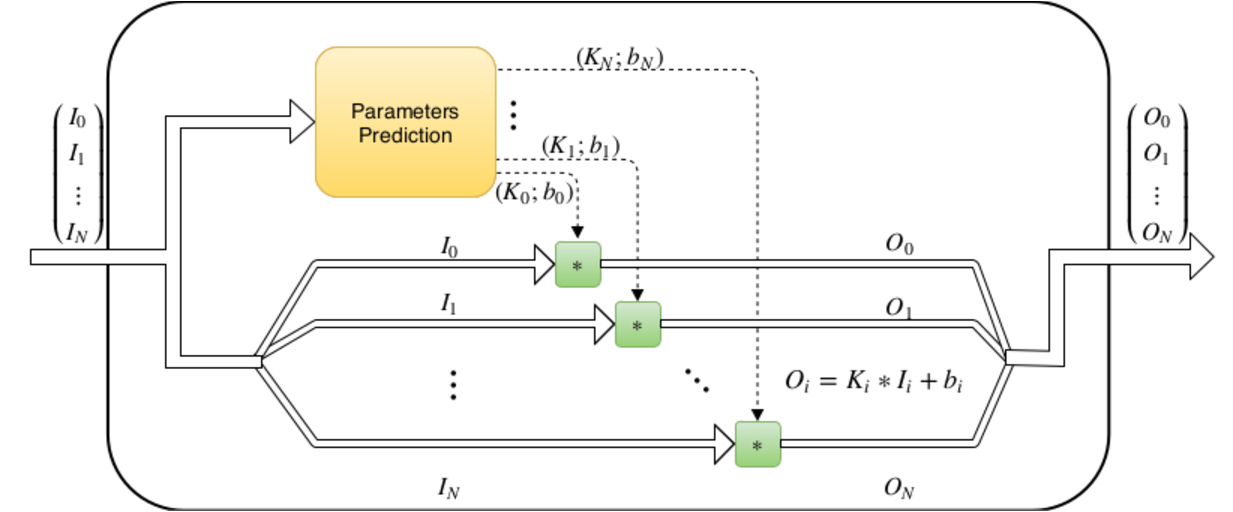
\includegraphics[width=\textwidth]{img_transfer/Intensity_Block}
    \caption{Intensity Layer. ``Parameters Prediction'' can be any model, in our case it is a 3-layers ConvNet.}
    \label{fig:block}
\end{figure}

A geometric transformation is not enough to express the differences between the source and target datasets. We therefore propose to predict an intensity transformation, implemented as a $1 \times 1 \times 1$ convolution applied to each feature map, shown in Figure~\ref{fig:block}. The exact transformation applied to each feature map $I_i$ is:
\begin{equation*}
O_i = K_i \left( I; \theta \right) * I_i + b_i \left( I; \theta \right)
\end{equation*}
where $K_i \left( I; \theta \right)$ and $b_i \left( I; \theta \right)$ are the parameters predicted. In the end, two parameters have to be predicted for each feature map. Experiments showed that this layer works best when placed at the lowest level of the U-Net (see Figure~\ref{fig:unet}).

%%%%%%%%%%%%%%%%%%%%%%%%%%%%%%%%%%%%%%%%%%%%%%%%%%%%%%%%%%%%%%%%%%%%%%%%%%%%%%%%%%%%%%%%%%%%%%%
\section{Application: Kidney Segmentation in 3D Ultrasound}
\label{sec:kidney_seg}

%%%%%%%%%%%%%%%%%%%%%%%%%%%%%%%%%%
\subsection{Introduction}

A common (and often disappointing) scenario in clinical settings is to expect an algorithm, built on a specific class of medical images, to succeed at the same task on data judged similar by the clinician. Focusing on the particular class of deep learning-based methods, we propose a transfer approach to, if not instantly, quickly satisfy this expectation. We work under the assumption that no access to the original training database is possible, as it is frequently the case in practice. 

The clinical problem motivating this work is the kidney capsule segmentation in 3D ultrasound data from potentially ill children. These images have a high amount of noise, strong dependency on the operator, and important organ shape variability induced by subjects age and degree of illness. Moreover we have limited access to such volumes. In contrast, a much larger database of ultrasound kidney volumes of healthy adults is available, from which we build a successful segmenting deep network. We aim to transfer this network knowledge. % to the pediatric data. 

This work has contributions in both the clinical and technical domains: (i) a deep learning based algorithm for kidney capsule segmentation in 3D ultrasound data (Section~\ref{sssec:unet}), and (ii) a new approach to perform domain transfer of a pre-trained neural network (Section~\ref{sssec:transfer}). In addition we present experiments comparing different transfer methods according to performance, training time and added complexity to determine the trade-offs of each method (Section~\ref{ssec:exp}), and discuss their results, examining the segmentation errors to suggest potential improvements.

%%%%%%%%%%%%%%%%%%%%%%%%%%%%%%%%%%
\subsection{Related Work}

%\subsubsection{Kidney segmentation in 3D ultrasound data}

Despite the clinical potential of 3D kidney ultrasounds, both the number of publications and the data used within are relatively small. Moreover, to the best our knowledge, deep learning techniques have not yet been applied.~\textcite{cerrolaza2014ISBI} and~\textcite{marsousi2017} have addressed the capsule segmentation problem in 3D pediatric data using active shape models and for real-time segmentation using implicit deformable models, respectively. 
%In fact, we have not found any paper using deep learning for the segmentation of the kidney in 3D ultrasound.
Nevertheless, deep learning techniques have been applied by~\textcite{ravishankar2017MICCAI} to 2D ultrasound kidney images. Their approach is compelling since they manage to combine deep learning and shape priors by using two networks, first a U-Net for the segmentation, then a convolutional auto-encoder as a shape prior used for regularization.

The baseline to our work (Section~\ref{sssec:baseline}) is the well-known deep learning architecture ``U-Net'' (\textcite{ronneberger2015MICCAI}) and its 3D version (\textcite{cicek2016MICCAI}). 

%DeepMedic is another framework developed for the segmentation of lesions in 3D MR brain images by Kamnitsas \textit{et al.}~\cite{kamnitsas_2017}. The segmentation is done in two parts, first the image go through a 3D convolutional neural network that outputs a segmentation map, which is then refined by a 3D conditional random field. Additionally, the CNN takes as input the image at normal resolution and a down-sampled version in order to incorporate multi-scale features.

%%%%%%%%%%%%%%%%%%%%%%%%%%%%%%%%%%
\subsection{Methods}

\subsubsection{Baseline}
\label{sssec:unet}

The 3D extension (\textcite{cicek2016MICCAI}) of the U-Net (\textcite{ronneberger2015MICCAI}) architecture is our starting point. Its symmetrical structure alternates convolutional layers with down-sampling layers on one side and convolutional layers with up-sampling layers on the other (see Figure~\ref{fig:unet}). At each level, down-sampled feature maps are concatenated to up-sampled ones to enforce attachment to the data. In our adaptation of this architecture we replace the weighted softmax loss by a Dice-based loss, more adapted to our segmentation task. Moreover, introducing Spatial Dropout (\textcite{tompson2015CVPR}) after each convolution-sampling block proved to significantly improve our results by preventing over-fitting.

\begin{figure}
	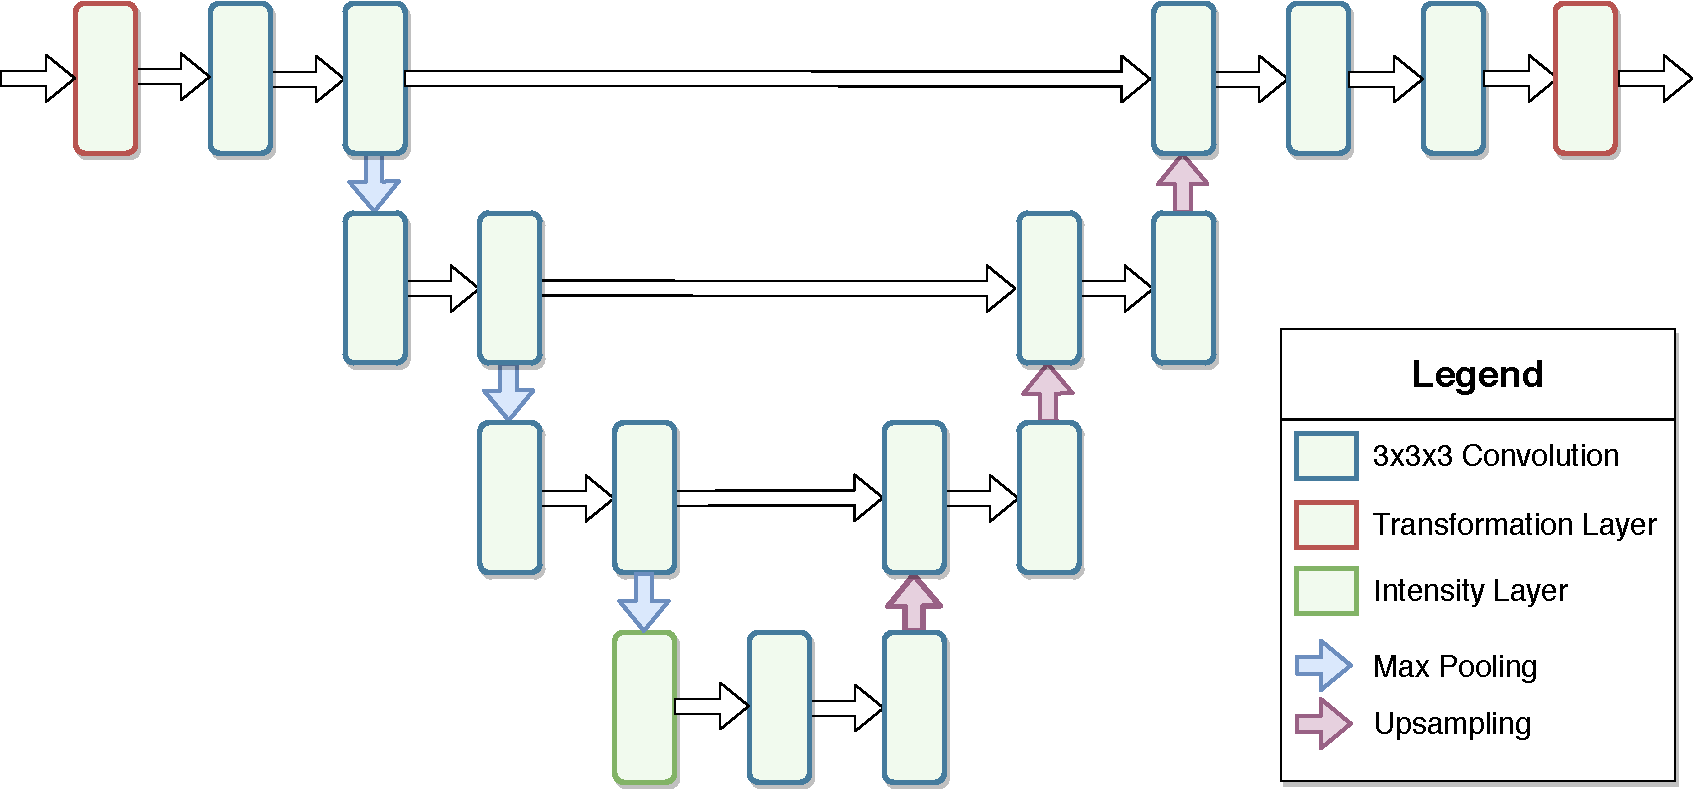
\includegraphics[width=0.9\textwidth]{img_transfer/UNet}
    \caption{U-Net structure with our added transformation and intensity layers.}
    \label{fig:unet}
\end{figure}

%We also train the network with Spatial Dropout after each block, just before the down and up-sampling layers. Standard Dropout~\cite{srivastava_2014} is a regularization method that works by randomly setting a group of neurons at zero after each batch during training. This helps reducing over-fitting by preventing neurons from becoming strongly correlated. But this has no effect on convolutional layers as inputs are spatially correlated. A solution is to use Spatial Dropout~\cite{tompson_2015} which, instead of dropping neurons, drops entire feature maps.

%%%%%%%%%%%%%%%%%%%%%%%%%%%%%%%%%%
\subsubsection{Transfer Learning with Transformation Layers}
\label{sssec:transfer}

Having successfully trained a network on kidney adults data we seek to transfer its knowledge into a new model that will correctly segment pediatric kidneys and still have good performances on adults. Fine tuning is a poor option in our case since it degrades the performance on the adult images.



%%%%%%%%%%%%%%%%%%%%%%%%%%%%%%%%%%
\subsection{Experiments and Results}
\label{ssec:exp}

%%%%%%%%%%%%%%%%%%%%%%%%%%%%%%%%%%
\subsubsection{Dataset}
\label{sssec:data}

The ultrasound volumes in our study come from several clinical sites around the world.
As a result, there is a high variability in the quality of the images, which translates into various amounts of noise and shadows artifacts.

We have a total of 503 healthy adults images, and 64 children, of which about $30 \%$ have hydronephrosis in various stages. The database was split into $80 \%$ of the images used for training, the rest for testing.

The volumes we give to the network have been down-sampled to a resolution of $4 \times 4 \times 4$ mm$^3$, and centered in a $80 \times 80 \times 80$ voxels cube. The size in voxels was chosen in order to fit the network and a volume on a single NVIDIA TITAN GPU. The resolution was chosen so that each volume would fit entirely in the cube. 
%Because we are not segmenting fine structures but only the kidneys, a smaller resolution is not vital.

%%%%%%%%%%%%%%%%%%%
\subsubsection{Baseline}
\label{sssec:baseline}

We used Keras (\textcite{chollet2015keras}) with the Tensorflow backend (\textcite{tensorflow2015}). We performed each experiment on five seeds, which impacts both the separation of the data set into training and test sets, and the initialization of the weights of the networks.

Three models are used as baseline: one trained on adults kidneys only, which will also be used for transfer, one trained on children only, and one trained on both, with oversampling of the children to balance each set. Oversampling is a common way of dealing with class imbalance (\textcite{buda2017}) and consists in balancing each epoch to have as many adults as children by drawing each children multiple times.

These baselines allow us to judge the quality of each transfer method. A good transfer method should perform better (or close to) on the children kidneys than the children only network, while staying close to the performance of the adults only network on the adults. The joint model represents the ideal performance we can hope for on adults and children. Results are displayed in Table~\ref{table:results}, and illustrated in Figure~\ref{fig:mseg}.

%%%%%%%%%%%%%%%%%%%
\subsubsection{Comparing transfer methods}

\begin{table}
	\centering
\begin{tabular}{|l|c|c|c|c|}
	\hline
    Strategy & \# params & Time & Dice Adults & Dice Children \\
	\hline
    Adults Baseline & 16M & 900 & $\bm{0.80 \pm 0.01}$ & $0.61 \pm 0.02$ \\
    Children Baseline & 16M & 112 & $0.57 \pm 0.03$ & $\bm{0.66 \pm 0.02}$ \\
    Joint Baseline & 16M & 1790 & $\bm{0.81 \pm 0.01}$ & $\bm{0.74 \pm 0.01}$ \\
    \hline
    Fine tuning & 0 & 115 & $0.72 \pm 0.02$ & $0.72 \pm 0.03$ \\
    %5 & Add layers & a & 1 & 655k & 47 & $0.72 \pm 0.02$ & $0.66 \pm 0.03$ \\
    %6 & Add layers & a & 3 & 860k & 75 & $0.70 \pm 0.02$ & $0.67 \pm 0.03$ \\
    %7 & Add layers & b & 1 & 17M & 61 & $0.72 \pm 0.02$ & $0.70 \pm 0.02$ \\
    Convolutions everywhere & 23M & 182 & $0.71 \pm 0.02$ & $0.72 \pm 0.03$ \\
    %9 & Residual Convolution & 1.4M & 49 & $0.76 \pm 0.02$ & $0.65 \pm 0.03$ \\
    %10 & Add layers & d & 1 & 9 & 30 & $\bm{0.80 \pm 0.01}$ & $0.61 \pm 0.02$ \\
    %11 & Add layers & d & 3 & 27 & 88 & $\bm{0.80 \pm 0.01}$ & $0.62 \pm 0.02$ \\
    %12 & Add layers & e & 1 & 76k & 31 & $0.78 \pm 0.01$ & $0.65 \pm 0.03$ \\
    %13 & Add layers & e & 3 & 1.4M & 78 & $0.67 \pm 0.05$ & $0.65 \pm 0.07$ \\
    Geometric Input & 148k & 36 & $0.73 \pm 0.02$ & $0.67 \pm 0.02$ \\
    Intensity & 124k & 29 & $0.80 \pm 0.01$ & $0.65 \pm 0.03$ \\
    Geometric Input + Intensity & 272k & 37 & $\bm{0.74 \pm 0.01}$ & $\bm{0.73 \pm 0.02}$ \\
    \hline
\end{tabular}
	\vspace{2mm}
	\caption{Performance of the baseline and the different transfer methods. Each result is averaged over 5 random seeds impacting the separation of the database into training and testing sets, and the weights initialization of the networks.}
    \label{table:results}
\end{table}

% Table index: seed 42, 51, 1337, 3333, 123456
% Residual conv: version c, depth 1
% Geometric input: 62, 97, 64, 46, 26
% Intensity: 63, 98, 65, 47, 27
% geo + intensity: 61, 96, 63, 45, 25
% data aug: +5% everywhere

% 61, 68, 69, 59, 68

In all transfer experiments, the source network is the adults baseline. The transfer is done only on the children dataset, but performances are evaluated on both the adults and children datasets. Besides  fine tuning, we experimented with the types of layers added to the network and their position as described in Section~\ref{sssec:transfer}. The most interesting results are presented below.

In this section, we show that some of the proposed models achieve good results, both quantitatively as shown in Table~\ref{table:results} and qualitatively, as illustrated in Figures~\ref{fig:bad_images} and~\ref{fig:mseg}.

Table~\ref{table:results} shows the best performing strategies among those we explored. 
%The version letter corresponds to the numbering in Figure~\ref{fig:block}, while the depth indicates in which places we added the transfer layers. A depth of 1 means that we added the layers only in the innermost block, while a depth of 3 means that we added layers up to the outermost block of the U-Net. 
The number of parameters is the number of parameters added by the method to the base network, and the time is the time it takes for one epoch (in seconds).

For the baselines, jointly training on adults and children gives better results than training on each class alone, or than any transfer method. We conclude that it is the method that should be used if we have access to both datasets at the same time. It can be noted that the performance gap on the children dataset between the adults baseline and the children baseline is smaller than between the children baseline and the joint baseline. This suggests that the quantity of available data is more important than its quality.

% \begin{figure}
% \centering
% \begin{subfigure}{.5\textwidth}
%   \centering
%   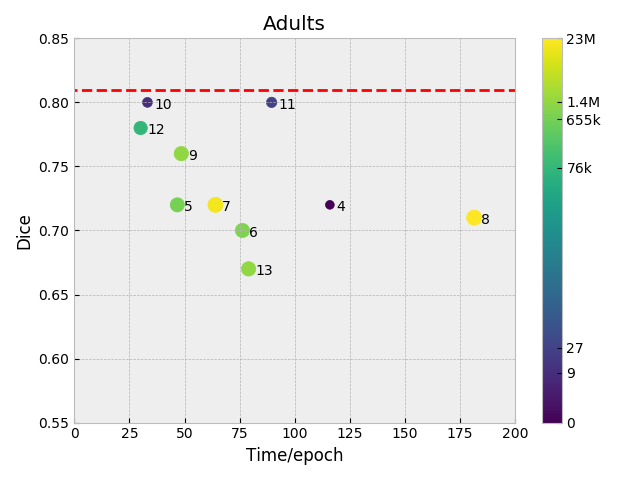
\includegraphics[width=\textwidth]{img/adults}
%   \caption{Dice index on adults}
% \end{subfigure}%
% \begin{subfigure}{.5\textwidth}
%   \centering
%   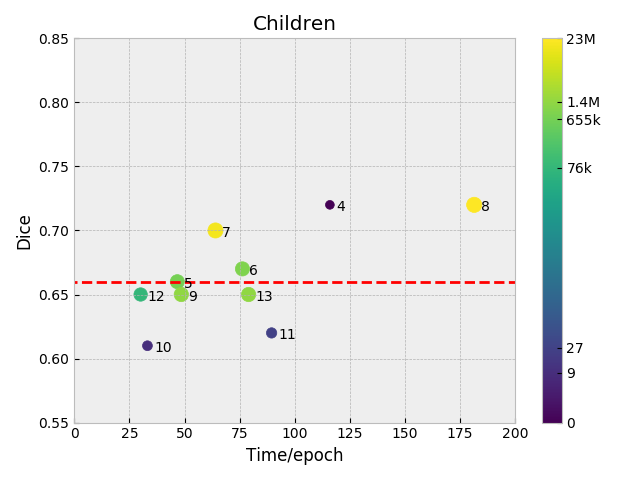
\includegraphics[width=\textwidth]{img/children}
%   \caption{Dice index on children}
% \end{subfigure}
% \caption{Comparing transfer methods. The x axis is the time in seconds taken by one epoch, the y axis is the Dice index. The color represents the number of trainable parameters in a logarithmic scale.}
% \label{fig:tradeoff}
% \end{figure}

%If we do not have access to the source dataset, we have to use a transfer method. Figure~\ref{fig:tradeoff} shows the performance of each transfer strategy compared to the baseline. Fine tuning works really well if we do not care about the performance on the source dataset. Otherwise, two models offering good trade-offs are numbers 9 and 12. Number 9 is surprising as the transfer blocks are residual, and in all other cases where we tried residual connections, it gave worse results.
%Number 12 uses only one transformation layer, therefore adding very few parameters and being fast to train. Surprisingly adding more transformation layers gives worse results as number 13 shows.

%Number 7 and 8 seem appealing on first sight as they give results similar to fine tuning, but at the cost of adding more parameters to the network than it had originally. 

For the transfer methods, the fine tuning easily beats the children baseline, but does not reach the performance of the joint baseline on either dataset. Moreover, while it does not add any parameter to the network, it takes more time to train than most other transfer methods (this is due to the fact that we have to compute the gradient of every parameter in the network).

Adding fixed convolutional layers did not work (a, b and c in Figure~\ref{fig:block}. We were able to reach the performance of the fine tuning, but only by adding $3 \times 3 \times 3$ convolutional layers at every position shown in Figure~\ref{fig:unet} (line  ``Convolutions everywhere'' in Table~\ref{table:results}).  This added 23 millions parameters to the network (it originally had 16 millions) and took longer to train than the fine tuning.

``Geometric Input'' means that we predict the parameters of a geometric transformation before the first layer of the network as described in Section~\ref{sssec:transfer}. It is fast to train and beats the children baseline but fine tuning gives better performance. Likewise for ``Intensity'' only, which means putting an intensity layer at the deepest layer of the U-Net.

The best results were obtained by combining the geometric input and learning to predict the parameters of an intensity transformation of the feature maps at the lowest level of the U-Net. This position for the intensity transformation works better than the others. This method adds a small amount of parameters, is fast to train and improve the performance more than fine tuning.

%%%%%%%%%%%%%%%%%%%
\subsubsection{Examining common failures}

% \begin{figure}[ht]
%   \begin{subfigure}[b]{0.5\linewidth}
%     \centering
%     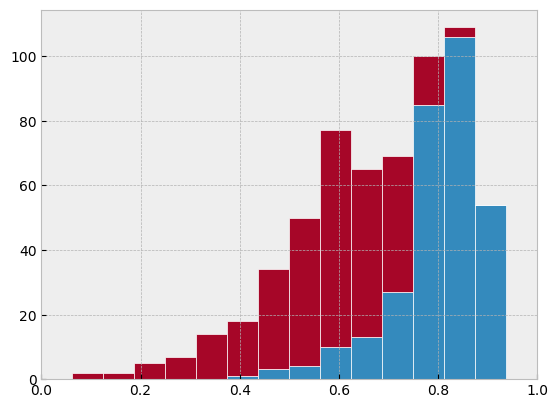
\includegraphics[width=0.95\linewidth]{img/hist_adults} 
%   \end{subfigure}%% 
%   \begin{subfigure}[b]{0.5\linewidth}
%     \centering
%     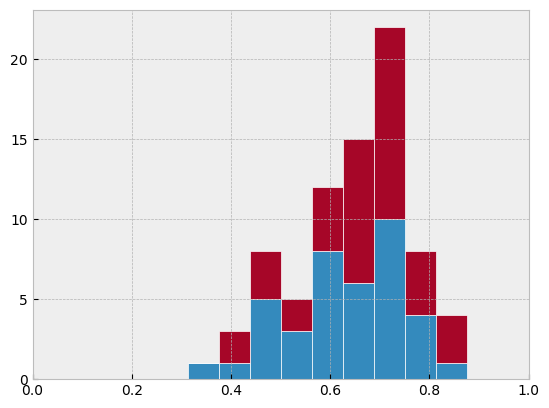
\includegraphics[width=0.95\linewidth]{img/hist_children} 
%   \end{subfigure} 
%   \caption{Histogram of Dice coefficient on baseline models. In red is the adults baseline, blue is the children baseline. Left: Dice coefficient on adults, right: Dice coefficient on children.}
%   \label{fig:hist} 
% \end{figure}

\begin{figure}
\centering
\begin{subfigure}{.33\textwidth}
  \centering
  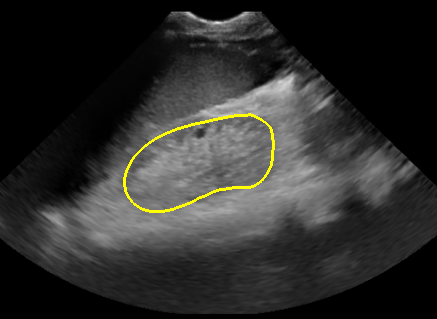
\includegraphics[width=.95\textwidth]{img_transfer/adult_bad}
\end{subfigure}%
\begin{subfigure}{.33\textwidth}
  \centering
  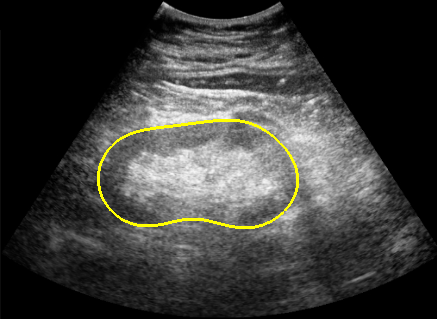
\includegraphics[width=.95\textwidth]{img_transfer/adult_less_bad}
\end{subfigure}
\begin{subfigure}{.33\textwidth}
  \centering
  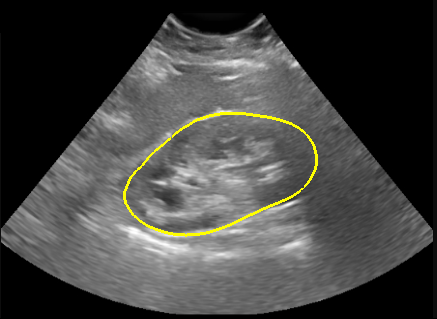
\includegraphics[width=.95\textwidth]{img_transfer/child_less_bad}
\end{subfigure}
\caption{Images on which all models fail to generalize well.}
\label{fig:bad_images}
\end{figure}

Examining in details the results of the different networks, we can observe a few trends. 
%From the histograms of the Dice coefficient in Figure~\ref{fig:hist}, 
Looking at each image individually, we note that a few of them have a very low Dice index ($< 0.20$). We show some of these images in Figure~\ref{fig:bad_images}. Moreover they are consistently bad for all tested models. All three images are of very low quality, and there are shadows hiding parts of the images. Fortunately, they represent less than $1 \%$ of our dataset.

\begin{figure}
	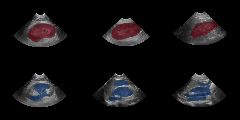
\includegraphics[width=\textwidth]{img_transfer/seg_good_bad}
    \caption{Middle slice of 6 different volumes and a network segmentation superposed on it. The top row shows good segmentations with a Dice index $> 0.90$. The bottom row shows segmentations with a Dice index between $0.60$ and $0.70$. They show the most common mistakes made by the network.}
    \label{fig:mseg}
\end{figure}

Looking at the other images, two kinds of failures were dominant. Either there were holes in the segmentation or the segmentation were bigger than the ground truth. Some of these mistakes are shown in Figure~\ref{fig:mseg}. The holes in the segmentation result from a lack of constraint on the shape of the segmentation. A big segmentation containing the ground truth or a segmentation with holes can have a high dice value. Adding constraints to the loss could also help to solve some of the common mistakes. Other ways to alleviate the problem would be to smooth the segmentations or to use a shape model, for example using a Conditional Random Field such as in~\textcite{kamnitsas2017MEDIA}.

%%%%%%%%%%%%%%%%%%%%%%%%%%%%%%%%%%
\subsection{Conclusion}
\label{ssec:conclusion}

We proposed a new transfer method taking advantage of the particularity of the image format of our problem to obtain better results than the more generic fine-tuning. This new method could be applied to other medical imaging problems, with a few caveats. First, if access to the source dataset is possible, joint training on the source and target should be preferred over any transfer method. Second, if changes to the structure of the network are impossible (for example if the architecture is hard-coded in released software), our method cannot be used. Finally, it depends on the nature of the differences between the source and target distributions. Our method is efficient in the case of geometric and/or intensity differences, making it well suited for medical imaging problems.


%%%%%%%%%%%%%%%%%%%%%%%%%%%%%%%%%%%%%%%%%%%%%%%%%%%%%%%%%%%%%%%%%%%%%%%%%%%%%%%%%%%%%%%%%%%%%%%
%                                        SEGMENTATION                                         %
%%%%%%%%%%%%%%%%%%%%%%%%%%%%%%%%%%%%%%%%%%%%%%%%%%%%%%%%%%%%%%%%%%%%%%%%%%%%%%%%%%%%%%%%%%%%%%%
\chapter{Deformable Shape Models using Deep Learning}
\label{chap:seg}

\begin{chapabstract}
 Coucou
\end{chapabstract}

\vspace{1cm}

{   
    \setstretch{1.0}
    \minitoc
}

\newpage

%%%%%%%%%%%%%%%%%%%%%%%%%%%%%%%%%%%%%%%%%%%%%%%%%%%%%%%%%%%%%%%%%%%%%%%%%%%%%%%%%%%%%%%%%%%%%%%
\section{Deformable shape models}

\subsection{Before deep learning}

\begin{itemize}
    \item Link with registration ?
\end{itemize}

\subsection{Building a shape model}

\subsection{Deforming the shape model}

An Unsupervised Learning Model for Deformable Medical Image Registration



%%%%%%%%%%%%%%%%%%%%%%%%%%%%%%%%%%%%%%%%%%%%%%%%%%%%%%%%%%%%%%%%%%%%%%%%%%%%%%%%%%%%%%%%%%%%%%%
\section{Deformable shape models and deep learning}

We propose in this section to train a neural network to predict the deformation required for a shape model to match a segmentation target on a specific image. There are two components: predicting a geometric transformation and predicting the deformation field.

\begin{figure}[htbp]
	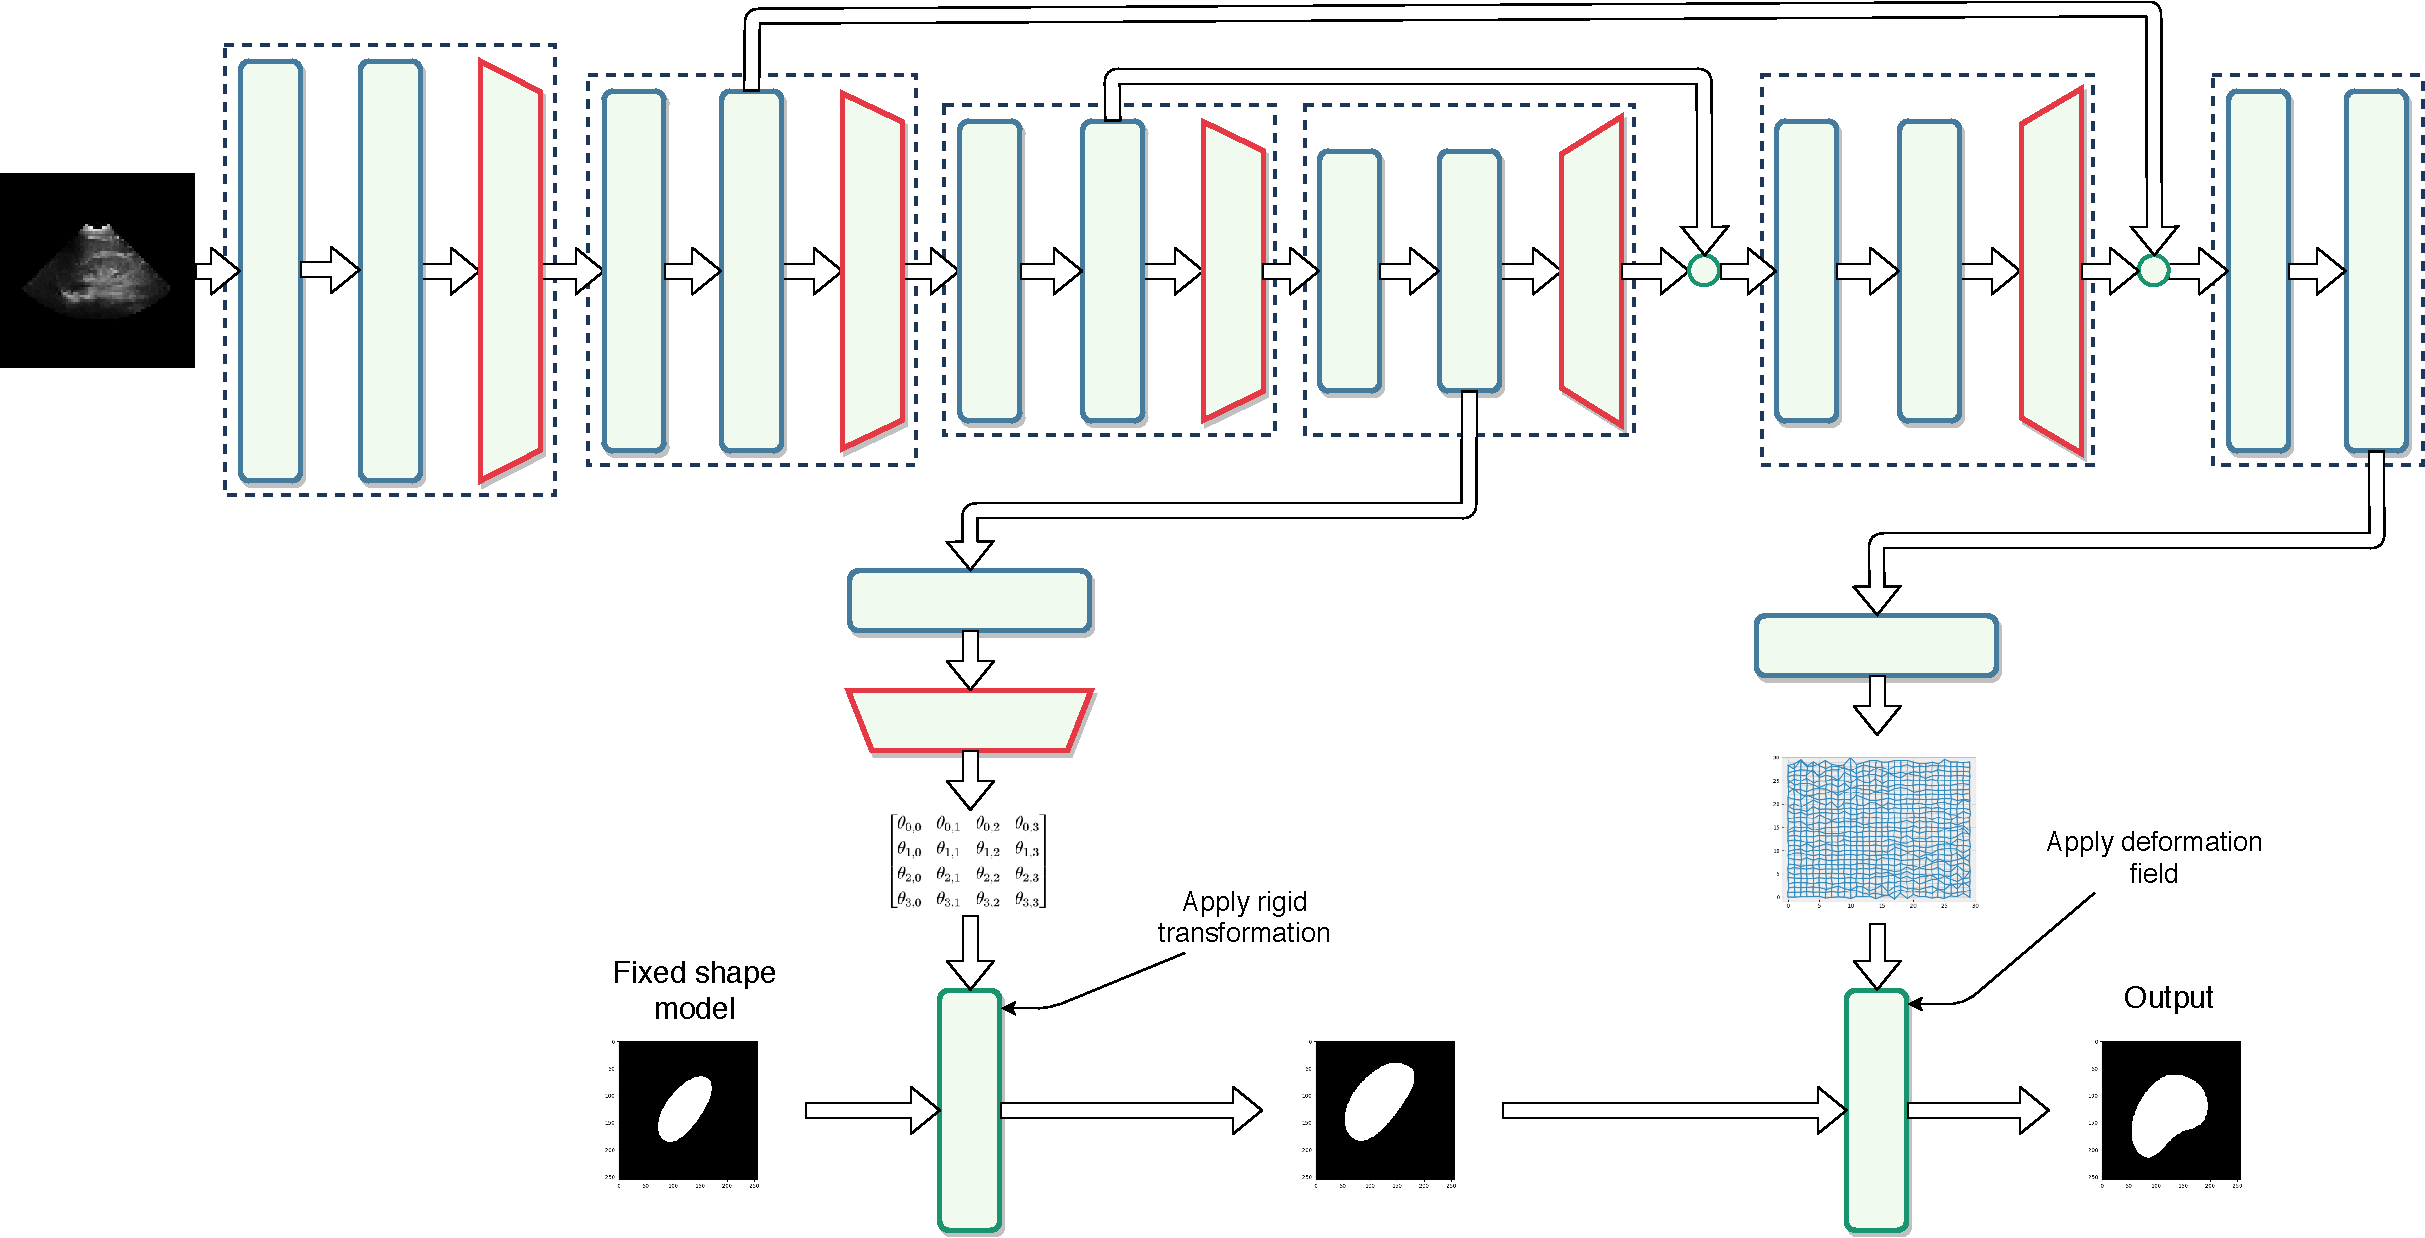
\includegraphics[width=\textwidth]{img_seg/deformation_network}
    \caption{Segmentation network that predicts a geometric transformation and a deformation field to deform a shape model.}
    \label{fig:deform_network}
\end{figure}

Figure~\ref{fig:deform_network} presents the process. The network predict a geometric transformation and a deformation field from the image, which are applied to a fixed shape model. The deformed shape model then corresponds to the correct segmentation for the image. The shape model is simply the ground truth segmentation from an image not included in the training, validation or test sets.

The next sections explains how to predict and apply the transformation and the deformation field.

\subsection{Predicting a geometric transformation}

A geometric transformation for 3D images is represented by a $4 \times 4$ matrix, meaning a total of 16 parameters that can be predicted. Directly predicting those parameters remove control on the kind of transformation that are predicted. In our case, we chose to predict instead translation, rotation and scaling parameters. 

Three parameters are predicted for the translation on each axis, giving the following translation matrix $T$:
\begin{equation*}
    T = 
    \begin{bmatrix}
        1 & 0 & 0 & t_x \\
        0 & 1 & 0 & t_y \\
        0 & 0 & 1 & t_z \\ 
        0 & 0 & 0 & 1
    \end{bmatrix}
\end{equation*}

The scaling matrix $S$ is built from three more parameters:
\begin{equation*}
    S = 
    \begin{bmatrix}
        s_x & 0 & 0 & 0 \\
        0 & s_y & 0 & 0 \\
        0 & 0 & s_z & 0 \\ 
        0 & 0 & 0 & 1
    \end{bmatrix}
\end{equation*}

Finally, we have one rotation matrix in each direction ($R_x$, $R_y$ and $R_z$) built from one parameter each:
\begin{align*}
    R_x &= 
    \begin{bmatrix}
        1 & 0 & 0 & 0 \\
        0 & \cos{r_x} & -\sin{r_x} & 0 \\
        0 & \sin{r_x} & \cos{r_x} & 0 \\ 
        0 & 0 & 0 & 1
    \end{bmatrix} \\
    R_y &= 
    \begin{bmatrix}
        \cos{r_y} & 0 & - \sin{r_y} & 0 \\
        0 & 1 & 0 & 0 \\
        \sin{r_y} & 0 & \cos{r_y} & 0 \\ 
        0 & 0 & 0 & 1
    \end{bmatrix} \\
    R_z &= 
    \begin{bmatrix}
        \cos{r_z} & -\sin{r_z} & 0 & 0 \\
        \sin{r_z} & \cos{r_z} & 0 & 0 \\
        0 & 0 & 1 & 0 \\ 
        0 & 0 & 0 & 1
    \end{bmatrix}
\end{align*}

We also need to center the image around zero before applying the rotations, which requires no parameters except knowing the center of the image:
\begin{equation*}
    C_+ = 
    \begin{bmatrix}
        1 & 0 & 0 & c_x \\
        0 & 0 & 0 & c_y \\
        0 & 0 & 0 & c_z \\ 
        0 & 0 & 0 & 1
    \end{bmatrix}
    \mkern20mu
    C_- = 
    \begin{bmatrix}
        1 & 0 & 0 & -c_x \\
        0 & 0 & 0 & -c_y \\
        0 & 0 & 0 & -c_z \\ 
        0 & 0 & 0 & 1
    \end{bmatrix}
\end{equation*}

From these matrices, the geometric transformation $G$ applied to the shape model is the following:
\begin{equation}
    G = T \cdot C_+ \cdot R_z \cdot R_y \cdot R_x \cdot S \cdot C_-
\end{equation}

The prediction of the 9 required parameters is done by a convolutional layer with 9 $1 \times 1 \times 1$ filters, followed by an average pooling layer of the size of the feature maps. 

\subsection{Predicting a deformation field}

The deformation field are predicted from a convolutional layer with 3 $3 \times 3 \times 3$ filters, one filter per dimension. Each field is then smoothed with a $3 \times 3 \times 3$ mean filter, before being resized to the shape model size with a tri-linear interpolation. This resizing step allows predicting deformation fields at a lower resolution than the shape model, saving time and parameters to learn.

% While no constraints are applied to the fields in the end, we investigated adding an $L_2$ penalty term to the deformation fields $F$ in the loss function:
% \begin{equation}
%     P = \lambda \sum_x \left( F - I \right)(x)^2
% \end{equation}

% This resulted in a drastic decrease in performance

\subsection{Distance map and loss}

- Distance map and appropriate loss

%%%%%%%%%%%%%%%%%%%%%%%%%%%%%%%%%%%%%%%%%%%%%%%%%%%%%%%%%%%%%%%%%%%%%%%%%%%%%%%%%%%%%%%%%%%%%%%
\section{Application to the segmentation of the kidney in 3D-US}

- dataset and preprocessing

TODO:
\begin{itemize}
    \item Compare global transfo alone, defo field alone, global + field
\end{itemize}




%%%%%%%%%%%%%%%%%%%%%%%%%%%%%%%%%%%%%%%%%%%%%%%%%%%%%%%%%%%%%%%%%%%%%%%%%%%%%%%%%%%%%%%%%%%%%%%
%                                         CONCLUSION                                          %
%%%%%%%%%%%%%%%%%%%%%%%%%%%%%%%%%%%%%%%%%%%%%%%%%%%%%%%%%%%%%%%%%%%%%%%%%%%%%%%%%%%%%%%%%%%%%%%
\chapter{Conclusion}
\label{chap:conclusion}

%%%%%%%%%%%%%%%%%%%%%%%%%%%%%%%%%%%%%%%%%%%%%%%%%%%%%%%%%%%%%%%%%%%%%%%%%%%%%%%%%%%%%%%%%%%%%%%
\section{Summary of the contributions}

The following contributions were presented in this thesis.

\paragraph*{An incremental Cholesky decomposition to reduce the cost of Bayesian optimization.}
Most of the computational cost of Bayesian optimization is in the inversion of the Gaussian process' Gram matrix. We exploited a particularity in the structure of this matrix specific to Bayesian optimization: each successive call adds new rows and columns while leaving the rest of the matrix unchanged. We have shown that this property stays true for the underlying Cholesky decomposition, and how to compute the new decomposition faster when the previous decomposition is available.

\paragraph*{A comparison of the performance of random search and Bayesian optimization.} 
We designed an experiment on a small hyper-parameter space to observe the behaviour of random search and Bayesian optimization over many runs. Bayesian optimization found better models than random search faster in the best, average and worst cases. We showed how the Gaussian process quickly became a good predictor of model performance and how the worst models were picked last. Random search behaved in accordance to the theoretical bounds we derived. Additionally we observed the distribution of models performance to be Gaussian.

\paragraph*{A new hyper-parameter optimization method combining Hyperband and Bayesian optimization.}
We proposed a method combining the strengths of Hyperband and Bayesian optimization. Model selection is done by Bayesian optimization, and model training follows Hyperband scheme. Unfortunately due to how the selection of multiple models simultaneously was handled, the method did not perform significantly better than Hyperband alone.

\paragraph*{A method to solve a classification problem of MRI field-of-view.}
Using a dataset of MRI volumes from a multitude of protocols and machines, we developed a neural network able to classify each slice of the volumes into their anatomical regions (such as head or pelvis). We improved on this neural network by using Bayesian optimization to find a better architecture providing a non-negligible performance boost. Even though the classification was done at the slice level, we showed how it could be used for robust region localization through a decision scheme maximizing the likelihood of each region.

\paragraph*{A new transfer learning method and its application to the segmentation of the kidney in 3D ultrasound images.}
Working with a dataset of 3D ultrasound kidney images across two populations, we investigated transfer learning methods for the segmentation of the kidney from one population (healthy adults) to the other (sick children). This led us to develop a new transfer learning approach, based on adding layers to the pre-trained network to predict parameters for geometric and intensity transformation. 

\paragraph*{A statistical shape model approach using deep learning.}
<TODO after chapter is done> 

%%%%%%%%%%%%%%%%%%%%%%%%%%%%%%%%%%%%%%%%%%%%%%%%%%%%%%%%%%%%%%%%%%%%%%%%%%%%%%%%%%%%%%%%%%%%%%%
\section{Future Work}

All of the contributions presented can be developed further as we discuss in this section.

\paragraph*{An incremental Cholesky decomposition to reduce the cost of Bayesian optimization.}
Even though we proved the complexity gain, we didn't integrate the incremental decomposition into a Bayesian optimization framework. This would be the next step, and would allow measuring the time gained in average. The testing could be done on the limited CIFAR-10 hyper-parameter space on which we compared random search and Bayesian optimization. As the gain in time becomes more important with the number of models tested, it might be interesting to increase the hyper-parameter space to a couple thousand models.

\paragraph*{A comparison of the performance of random search and Bayesian optimization.} 
Following the previous paragraph, extending the hyper-parameter space would yield insights into how Bayesian optimization behaves in larger spaces. This framework of testing could be used to observe the behaviour of other methods such as Hyperband. We observed models performance to be normally distributed, but the scope is limited to one hyper-parameter space on one task. To the best of our knowledge there is no theory on how to build good hyper-parameter spaces and understanding the relation between models, tasks and model performance would be of practical use to the use of hyper-parameter optimization methods.

\paragraph*{A new hyper-parameter optimization method combining Hyperband and Bayesian optimization.}
We have already described the flaws of our method: normalizing the acquisition function to transform it into a distribution from which we can draw multiple combinations resulted in a quasi-uniform distribution, completely negating the point of Bayesian optimization. Using a different strategy this combination method would perform better than either Hyperband or Bayesian optimization, as shown recently in~\textcite{falkner2018}.

\paragraph*{A method to solve a classification problem of MRI field-of-view.}
As the method presented gives robust results on our dataset, there is little need to improve it. It could be interesting however, to explore how to directly predict the boundaries of the regions using deep learning, instead of classifying each slice and using another method to obtain the regions. 

\paragraph*{A new transfer learning method and its application to the segmentation of the kidney in 3D ultrasound images.}
The limitation of the transfer learning method as presented is that it is highly specific to the kidney segmentation problem described. While the concept of adding specific transformation layers is general, it needs to be validated on other problems. 

\paragraph*{A statistical shape model approach using deep learning.}
<TODO after chapter is done> 


\begin{appendices}
    %%%%%%%%%%%%%%%%%%%%%%%%%%%%%%%%%%%%%%%%%%%%%%%%%%%%%%%%%%%%%%%%%%%%%%%%%%%%%%%%%%%%%%%%%%%%%%%
%                                          CHOLESKY                                           %
%%%%%%%%%%%%%%%%%%%%%%%%%%%%%%%%%%%%%%%%%%%%%%%%%%%%%%%%%%%%%%%%%%%%%%%%%%%%%%%%%%%%%%%%%%%%%%%
\chapter{Incremental Cholesky Decomposition Proofs}
\label{app:cholesky}

This appendix contains the derivations for obtaining the incremental Cholesky decomposition and its inverse that are used in Section~\ref{sec:cholesky}. For recall, the Cholesky decomposition and its inverse can be decomposed into blocks where one is the previous Cholesky decomposition. We obtain the formulas by developing this block decomposition.

Let us recall that the Cholesky decomposition $L_{(n)}$ of a positive definite matrix $K_{(n)}$ is a decomposition of the form:
\begin{equation}
	K_{(n)} = L_{(n)} L_{(n)}^T
\end{equation}
where $L_{(n)}$ is a lower triangular matrix. The decomposition is unique only if $K_{(n)}$ is positive definite. Since $K_{(n)}$ is a Gram matrix, it is always guaranteed to be positive semi-definite (i.e. $\forall v \in \mathbb{R}^n, \mkern10mu v^T K_{(n)} v \geq 0$). On top of that, if the rows and columns are unique (i.e. there are no duplicated data points), then it is positive definite.

%%%%%%%%%%%%%%%%%%%%%%%%%%%%%%%%%%%%%%%%%%%%%%%%%%%%%%%%%%%%%%%%%%%%%%%%%%%%%%%%%%%%%
\section[Formula for the Cholesky decomposition]{Formula for $L_{(n+k)}$}

When adding $k$ points to a Gram matrix of $n$ points, the block decomposition of the new Cholesky decomposition is:
\begin{alignat*}{2}
	&&L_{(n+k)} L_{(n+k)}^T &= K_{(n+k,n+k)} \\
	\Leftrightarrow\mkern40mu
	&&\begin{pmatrix}
    A & B \\
    C & D
  \end{pmatrix}
  \begin{pmatrix}
    A^T & C^T \\
    B^T & D^T
  \end{pmatrix} &= 
  \begin{pmatrix}
    K_{(n,n)} & K_{(k,n)}^T \\
    K_{(k,n)} & K_{(k,k)}
  \end{pmatrix}
\end{alignat*}
$B$ is obviously $0$ since a Cholesky decomposition is lower triangular.

By developing the block decomposition, we obtain the following equation for $A$:
\begin{equation*}
	A A^T + B B^T = A A^T = K_{(n,n)}
\end{equation*}
Since the Cholesky decomposition is unique, $A = L_{(n)}$. The equation for $C$ is also simple to solve:
\begin{alignat*}{2}
	&&C A^T + D B^T &= C L_{(n)}^T = K_{(k,n)} \\
	\Leftrightarrow\mkern40mu
	&&C &= K_{(k,n)} (L_{(n)}^T)^{-1}
\end{alignat*}
Solving for $D$ requires more work. Developing the block decomposition, we have:
\begin{alignat*}{2}
	&&C C^T + D D^T &= K_{(k,k)} \\
	\Leftrightarrow\mkern40mu
	&&D D^T &= K_{(k,k)} - K_{(k,n)} (K_{(n,n)})^{-1} K_{(k,n)}^T
\end{alignat*}
If we can show that $K_{(k,k)} - K_{(k,n)} (K_{(n,n)})^{-1} K_{(k,n)}^T$ is definite positive then $D$ is its unique Cholesky decomposition.

Let $w \in \mathbb{R}^{n+k} \quad \text{s.t.} \quad w = \begin{pmatrix}
    u \\
    v
  \end{pmatrix}, u \in \mathbb{R}^n, v \in \mathbb{R}^k$, we have $w^T K_{(n+k,n+k)} w \geq 0$ because $K_{(n+k,n+k)}$ is a Gram matrix. Using its block decomposition and developing it, we have:
\begin{alignat*}{2}
  &&\begin{pmatrix}
    u \\
    v
  \end{pmatrix} ^T
  \begin{pmatrix}
    K_{(n,n)} & K_{(k,n)}^T \\
    K_{(k,n)} & K_{(k,k)}
  \end{pmatrix}
  \begin{pmatrix}
    u \\
    v
  \end{pmatrix}
  &\geq 0 \\
  \Leftrightarrow\mkern40mu
  &&u^T K_{(n,n)} u + u^T K_{(k,n)}^T v +
  v^T K_{(k,n)} u + v^T K_{(k,k)} v
  &\geq 0 \\
  \Leftrightarrow\mkern40mu
  &&u^T K_{(n,n)} u + 
  2 u^T K_{(k,n)}^T v +
  v^T K_{(k,k)} v
  &\geq 0
\end{alignat*}
Using three successive change of variables, this equation becomes a second-order polynomial. The first change is $u = K_{(n,n)}^{-1} x$:
\begin{equation*}
  x^T (K_{(n,n)}^T)^{-1} x + 
  2 x^T (K_{(n,n)}^T)^{-1} K_{(k,n)}^T v +
  v^T K_{(k,k)} v
  \geq 0
\end{equation*}
The second change is $x = t y$ where $t$ is a scalar:
\begin{equation*}
  t^2 y^T (K_{(n,n)}^T)^{-1} y + 
  2 t y^T (K_{(n,n)}^T)^{-1} K_{(k,n)}^T v +
  v^T K_{(k,k)} v
  \geq 0
\end{equation*}
Since this is true for all $y \in \mathbb{R}^n$, this is true in particular when $y = K_{(k,n)}^T v$:
\begin{equation*}
  t^2 v^T K_{(k,n)} (K_{(n,n)}^T)^{-1} K_{(k,n)}^T v + 
  2 t v^T K_{(k,n)} (K_{(n,n)}^T)^{-1} K_{(k,n)}^T v +
  v^T K_{(k,k)} v
  \geq 0
\end{equation*}
The discriminant of this polynomial is negative or null because the polynomial is always positive or null:
\begin{align*}
  4 (v^T K_{(k,n)} (K_{(n,n)}^T)^{-1} K_{(k,n)}^T v)^2 -
  &4 (v^T K_{(k,n)} (K_{(n,n)}^T)^{-1} K_{(k,n)}^T v)
  (v^T K_{(k,k)} v)
  \leq 0 \\
  \Leftrightarrow\mkern20mu
  0 \leq (v^T K_{(k,n)} (K_{(n,n)}^T)^{-1} K_{(k,n)}^T v)^2
  &\leq 
  (v^T K_{(k,n)} (K_{(n,n)}^T)^{-1} K_{(k,n)}^T v)
  (v^T K_{(k,k)} v)
\end{align*}
$v^T K_{(k,k)} v \geq 0$ since $ K_{(k,k)}$ is a Gram matrix (i.e. positive semi-definite), meaning by necessity $v^T K_{(k,n)} (K_{(n,n)}^T)^{-1} K_{(k,n)}^T v \geq 0$ and $K_{(k,n)} (K_{(n,n)}^T)^{-1} K_{(k,n)}^T$ is positive semi-definite.

Moreover, $K_{(k,k)} \geq K_{(k,n)} (K_{(n,n)}^T)^{-1} K_{(k,n)}^T$, allowing us to conclude that $K_{(k,k)} - K_{(k,n)} (K_{(n,n)}^T)^{-1} K_{(k,n)}^T$ is positive semi-definite, and it is positive definite as long as none of the $k$ new combinations are duplicates of the $n$ previous combinations and $D D^T$ is its Cholesky decomposition.
\begin{equation*}
  D = cho(K_{(k,k)} - K_{(k,n)} (K_{(n,n)}^T)^{-1} K_{(k,n)}^T) = L_{(k)}
\end{equation*}
The final formula for the incremental Cholesky decomposition is:
\begin{equation}
  L_{(n+k)} = 
  \begin{pmatrix}
    L_{(n)} & 0 \\
    K_{(k,n)} (L_{(n)}^T)^{-1} & L_{(k)}
  \end{pmatrix}
\end{equation}
Since this formula requires the costly computation of $L_{(n)}^{-1}$, we would also like to find an incremental formula for it.

%%%%%%%%%%%%%%%%%%%%%%%%%%%%%%%%%%%%%%%%%%%%%%%%%%%%%%%%%%%%%%%%%%%%%%%%%%%%%%%%%%%%%
\section[Formula for the inverse Cholesky decomposition]{Formula for $L_{(n+k)}^{-1}$}

A standard expression for the inversion of a block matrix is:
\begin{equation*}
  \begin{pmatrix}
    A & B \\
    C & D
  \end{pmatrix}^{-1} = 
  \begin{pmatrix}
    A^{-1} + A^{-1} B (D - C A^{-1} B)^{-1} C A^{-1} & - A^{-1} B (D - C A^{-1} B)^{-1} \\
    - (D - C A^{-1} B)^{-1} C A^{-1} & (D - C A^{-1} B)^{-1}
  \end{pmatrix}
\end{equation*}
Simplifying with $L_{(n+k)}$ found previously, we have:
\begin{equation}
  L_{(n+k)}^{-1} =
  \begin{pmatrix}
    L_{(n)} & 0 \\
    K_{(k,n)} (L_{(n)}^T)^{-1} & L_{(k)}
  \end{pmatrix}^{-1} = 
  \begin{pmatrix}
    L_{(n)}^{-1} & 0 \\
    - L_{(k)}^{-1} K_{(k,n)} (L_{(n)}^T)^{-1} L_{(n)}^{-1} & L_{(k)}^{-1}
  \end{pmatrix}
\end{equation}

\end{appendices}

\cleardoublepage

%%%%%%%%%%%%%%%%%%%%%%%%%%%%%%%%%%%%%%%%%%%%%%%%%%%%%%%%%%%%%%%%%%%%%%%%%%%%%%%%%%%%%%%%%%%%%%%
%                                        BIBLIOGRAPHY                                         %
%%%%%%%%%%%%%%%%%%%%%%%%%%%%%%%%%%%%%%%%%%%%%%%%%%%%%%%%%%%%%%%%%%%%%%%%%%%%%%%%%%%%%%%%%%%%%%%
\nocite{*}

\defbibnote{clicknote}{Each header is a clickable link to the publication.}

\defbibnote{publinote}{This thesis resulted in the following publications.}

\printbibliography[prenote=publinote,heading=bibintoc,title={Publications},keyword=own]

\makeatletter\@openrightfalse
\printbibliography[prenote=clicknote,heading=bibintoc,title={Bibliography},notkeyword=own]
\@openrighttrue\makeatother 

\newcommand*\cleartoleftpage{%
   \clearpage
   \ifodd\value{page}\hbox{}\vspace*{\fill}\thispagestyle{empty}\newpage\fi
}
\cleartoleftpage

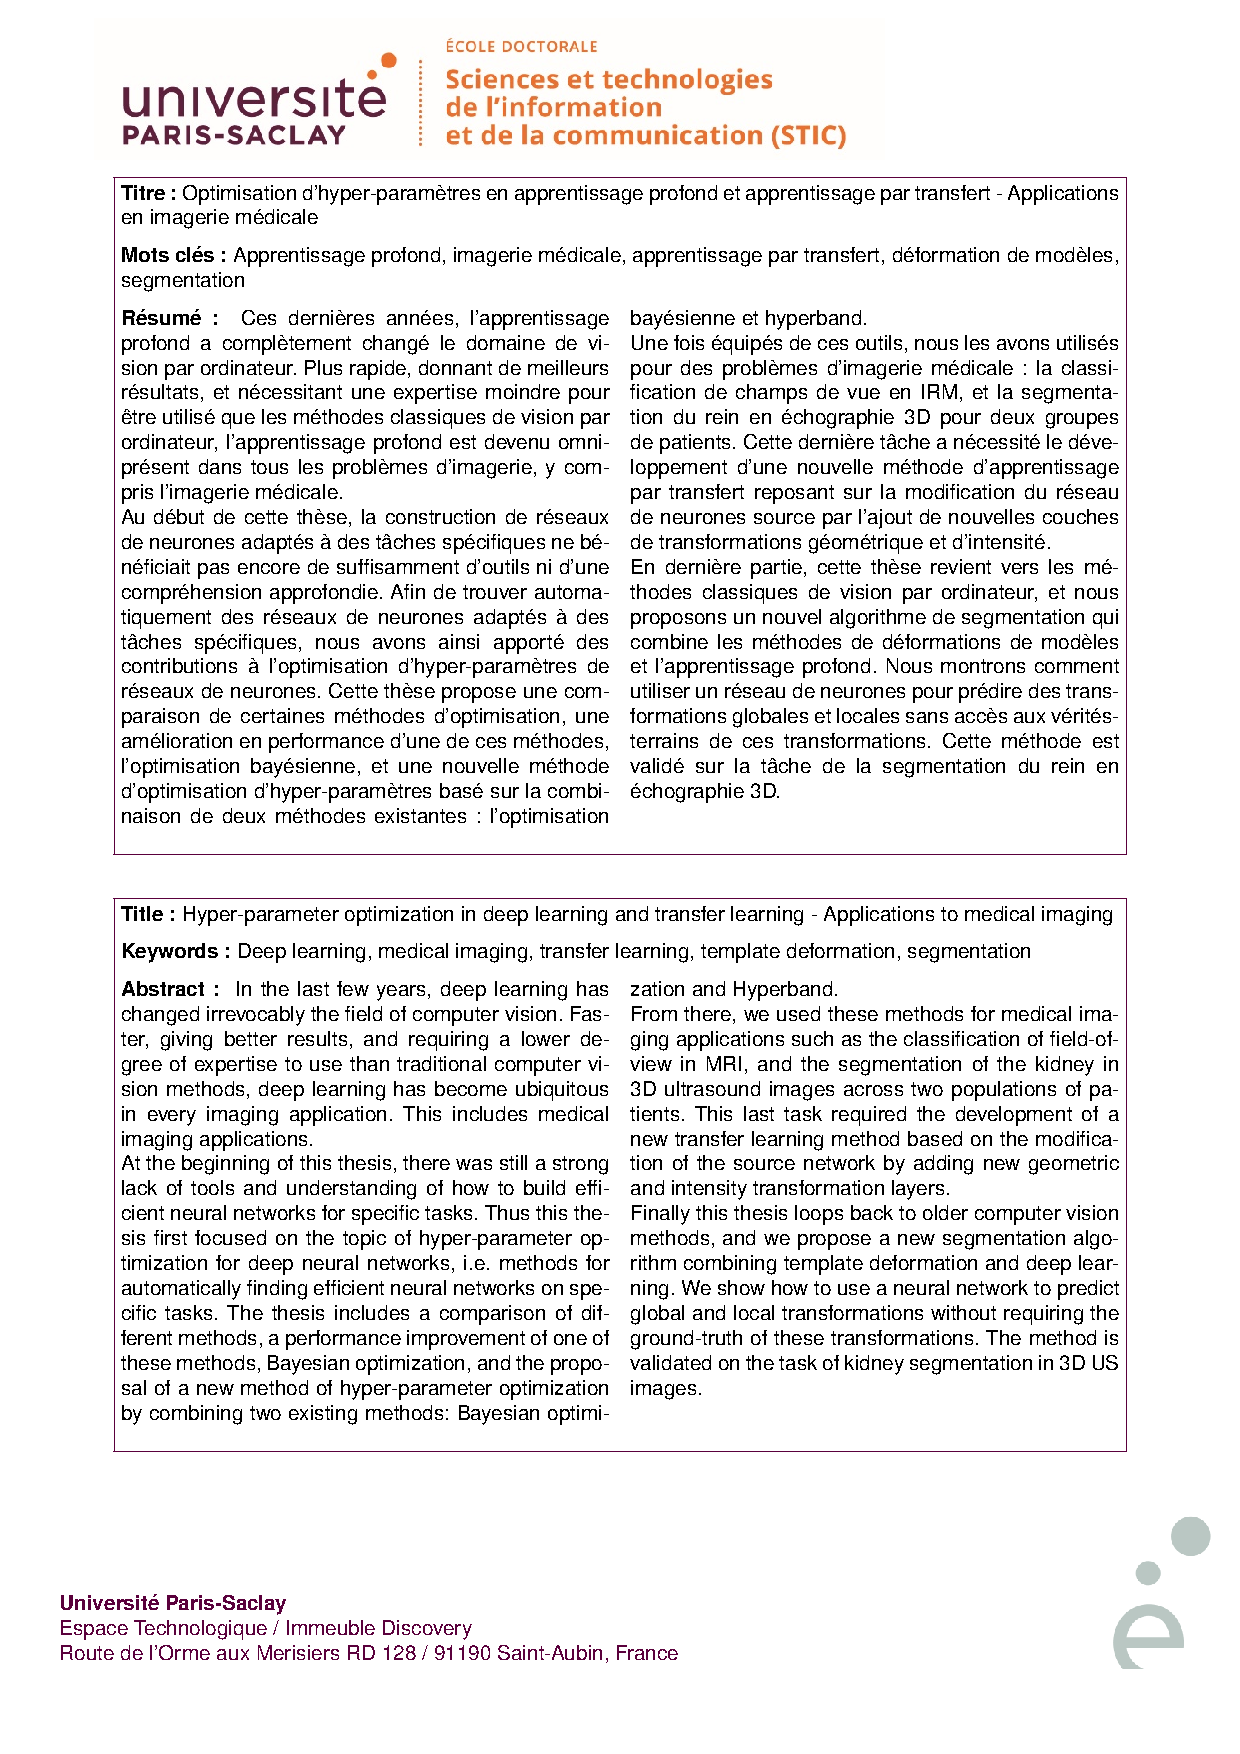
\includepdf{cover/4eme}

\end{document}
